%% This is the ctufit-thesis example file. It is used to produce theses
%% for submission to Czech Technical University, Faculty of Information Technology.
%%
%% This is version 1.6.0, built 18. 9. 2025.
%% 
%% Get the newest version from
%% https://gitlab.fit.cvut.cz/theses-templates/FITthesis-LaTeX
%%
%%
%% Copyright 2024, Tomas Novacek
%% Copyright 2021, Eliska Sestakova and Ondrej Guth
%%
%% This work may be distributed and/or modified under the
%% conditions of the LaTeX Project Public License, either version 1.3
%% of this license or (at your option) any later version.
%% The latest version of this license is in
%%  https://www.latex-project.org/lppl.txt
%% and version 1.3 or later is part of all distributions of LaTeX
%% version 2005/12/01 or later.
%%
%% This work has the LPPL maintenance status `maintained'.
%%
%% The current maintainer of this work is Tomas Novacek (novacto3@fit.cvut.cz).
%% Alternatively, submit bug reports to the tracker at
%% https://gitlab.fit.cvut.cz/theses-templates/FITthesis-LaTeX/issues
%%
%%

% arara: xelatex
% arara: biber
% arara: xelatex
% arara: xelatex

%%%%%%%%%%%%%%%%%%%%%%%%%%%%%%%%%%%%%%%%%
% CLASS OPTIONS
% language: czech/english/slovak
% thesis type: bachelor/master/dissertation/doctoral-report
% electronic (oneside) or printed (twoside), twoside is default
% paragraph - if passed, this optional argument sets paragraphs as the deepest level of headers, styles it, numbers it and adds it to Table of Content. Use with care! Normally, it is considered unwise to use it, since it is too deep.
% colour: bw for black&white OR no option for default colour scheme
%%%%%%%%%%%%%%%%%%%%%%%%%%%%%%%%%%%%%%%%%
\documentclass[english,bachelor,oneside]{ctufit-thesis}

%%%%%%%%%%%%%%%%%%%%%%%%%%%%%%%%%%
% FILL IN THIS INFORMATION
%%%%%%%%%%%%%%%%%%%%%%%%%%%%%%%%%%
\ctufittitle{Downscaling climate data with physically-constrained single-image super resolution} % replace with the title of your thesis
\ctufitauthorfull{Tomáš Becza} % replace with your full name (first name(s) and then family name(s) / surname(s)) including academic degrees
\ctufitauthorsurnames{Becza} % replace with your surname(s) / family name(s)
\ctufitauthorgivennames{Tomáš} % replace with your first name(s) / given name(s)
\ctufitsupervisor{Ing.\,Ondřej Podsztavek,\,Ph.D.} % replace with name of your supervisor/advisor (include academic degrees)
\ctufitdepartment{Department of Applied Mathematics} % replace with the department of your defence
\ctufitprogram{Informatics} % replace with your study program
\ctufitspecialisation{Artificial Intelligence 2021} % replace with your specialisation
\ctufityear{2026} % replace with the year of your defence
\ctufitdeclarationplace{Prague} % replace with the place where you sign the declaration
\ctufitdeclarationdate{\today} % replace with the date of signature of the declaration
\ctufitabstractCZE{
Predpovede klimatických dát sú väčšinou k dispozícii v rozlíšení od $0.44^\circ$ ($50$km) do $0.11^\circ$ ($12.5$km).
To je v súčasnej dobe už nedostatočné a preto sa výskum zaoberá zvyšovaním tohto rozlíšenia -- downscaling-om.
Avšak viaceré štúdie sa pri evaluácii príliš sústredia na pixel-wise chybu výstupu modelov a skutočnej hodnoty.
To môže nútiť modely produkovať fyzikálne nekonzistentné výstupy, len aby vyhoveli vyššie spomínanej pixel-wise stratovej funkcii.
Preto existujú takzvané fyzikálne obmedzenia ktoré, buď minimalizujú -- mäkké obmedzenia -- alebo kompletne zakazujú -- tvrdé obmedzenia -- nekonzistentné výstupy.
V tejto práci bolo odvodených niekoľko mäkkých obmedzení na základe konzistencie dilatačnej derivácie skrz downscaling.
Tieto obmedzenia, spolu s mäkkým a tvrdým obmedzením zákonu zachovania, sú v práci viacerými experimentmi ukázané ako úspešne vylepšujúce výkon modelov skrz rôzne typy obmedzení, veľkosti modelov ale aj škálovacích faktorov.
}
\ctufitabstractENG{
Climate data projections are available in the resolution from $0.44^\circ$ ($50$km) to $0.11^\circ$ ($12.5$km).
Currently, this is insufficient, therefore the resolution enhancing technique -- downscaling -- is involved.
However, various studies give a large accent on pixel-wise errors of downscaled images and targets.
That can force models to produce physically inconsistent outputs, only to minimize the pixel-wise loss function.
Thus, physical constraints are involved, which minimze -- soft constraints -- or completely forbid -- hard constraints -- incosistent outputs.
In this work more soft constraints were derived based on the dilated derivative consistency through downscaling.
These constraints, along with soft and hard constraint of conservation law, are by various experiment demonstrated as successfully improving the models' performances through constraint types, model sizes or scale factors.
}
\ctufitkeywordsCZE{klimatické dáta, downscaling, EDSR, soft-constrain\-ing, hard-con\-strain\-ing, physical-constraining, single-image super resolution}
\ctufitkeywordsENG{climate data, downscaling, EDSR, soft-constrain\-ing, hard-con\-strain\-ing, physical-constraining, single-image super resolution}
%%%%%%%%%%%%%%%%%%%%%%%%%%%%%%%%%%
% END FILL IN
%%%%%%%%%%%%%%%%%%%%%%%%%%%%%%%%%%

%%%%%%%%%%%%%%%%%%%%%%%%%%%%%%%%%%
% CUSTOMIZATION of this template
% Skip this part or alter it if you know what you are doing.
%%%%%%%%%%%%%%%%%%%%%%%%%%%%%%%%%%

\RequirePackage{iftex}[2020/03/06]
\iftutex % XeLaTeX and LuaLaTeX
    \RequirePackage{ellipsis}[2020/05/22] %ellipsis workaround for XeLaTeX
\else
    \errmessage{Only compilation with XeLaTeX or LuaLaTeX is allowed}
    \stop
\fi

% hyperlinks
\hypersetup{
    pdfpagelayout=TwoPageRight,
    colorlinks=false,
    allcolors=decoration,
    pdfborder={0 0 0.1}
}

% uncomment the following to hide all hyperlinks
%\hypersetup{hidelinks}

% uncomment the following to change the colour of all hyperlinks to CTU blue
%\hypersetup{allbordercolors=decoration}

\RequirePackage{pdfpages}[2020/01/28]

%%%%%%%%%%%%%%%%%%%%%%%%%%%%%%%%%%
% CUSTOMIZATION of this template END
%%%%%%%%%%%%%%%%%%%%%%%%%%%%%%%%%%


%%%%%%%%%%%%%%%%%%%%%%
% PACKAGES SETTINGS
% You may choose to modify this part.
%%%%%%%%%%%%%%%%%%%%%%
\usepackage{dirtree}
\usepackage{lipsum,tikz}
\usepackage[style=iso-numeric, maxbibnames=5, minbibnames=5]{biblatex}
\addbibresource{text/bib-database.bib}
\usepackage{xurl}
\usepackage{listings} % typesetting of sources
\usepackage{minted}
\usepackage{csquotes}
\usepackage{pdflscape}
\usepackage{subcaption}
\usepackage{array}
\usepackage{multirow}
\usepackage{hhline}
\usepackage{nicematrix}
\usetikzlibrary{decorations.pathreplacing}
\usepackage[final, verbose=silent]{microtype}

%%%%%%%%%%%%%%%%%%%%%%
% PACKAGES SETTINGS END
%%%%%%%%%%%%%%%%%%%%%%

\begin{document}
\frontmatter\frontmatterinit % do not remove these two commands

\thispagestyle{empty}\maketitle\thispagestyle{empty}\cleardoublepage % do not remove these four commands

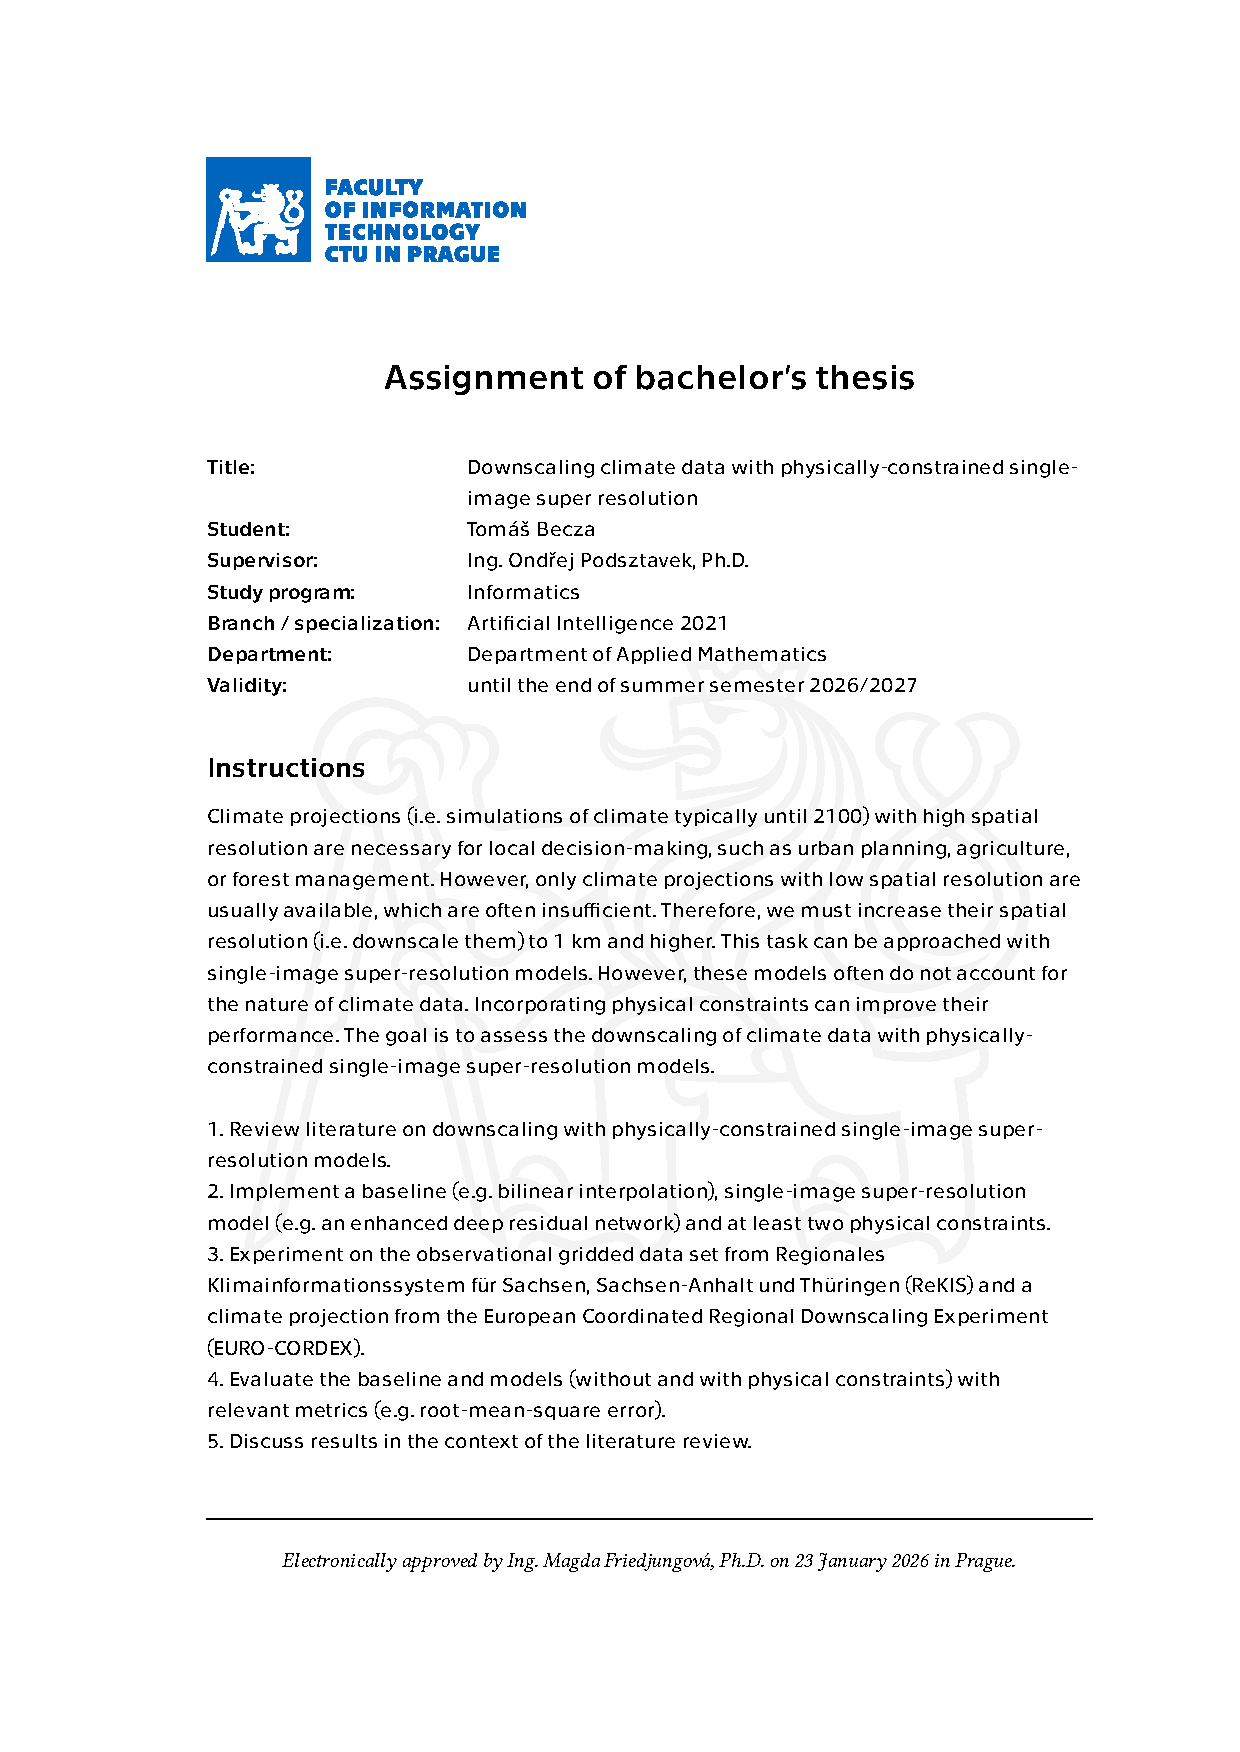
\includepdf[pages={1-}]{beczatom-assignment.pdf} % replace this file with your thesis assignment generated from ProjectsFIT

\imprintpage % do not remove this command
\stopTOCentries

%%%%%%%%%%%%%%%%%%%
% ACKNOWLEDGMENT
% FILL IN / MODIFY
% This is a place to thank people for helping you. It is common to thank your supervisor.
%%%%%%%%%%%%%%%%%%%
\begin{acknowledgmentpage}

    I would like to express my sincere gratitude to my supervisor, Ing.\,Ondřej Podsztavek,\,Ph.D., for the invaluable suggestions regarding the implementation and guidance throughout writing this thesis.
    My heartfelt thanks go to my parents, and my partner Tinka for always being there for me along the way, and their support when it got challenging.
\end{acknowledgmentpage}
%%%%%%%%%%%%%%%%%%%
% ACKNOWLEDGMENT END
%%%%%%%%%%%%%%%%%%%


%%%%%%%%%%%%%%%%%%%
% DECLARATION
% FILL IN / MODIFY
%%%%%%%%%%%%%%%%%%%
% INSTRUCTIONS
% ENG: choose one of approved texts of the declaration. DO NOT CREATE YOUR OWN. Find the approved texts at https://courses.fit.cvut.cz/SFE/download/index.html#_documents (document Declaration for FT in English)
% CZE/SLO: Vyberte jedno z fakultou schvalenych prohlaseni. NEVKLADEJTE VLASTNI TEXT. Schvalena prohlaseni najdete zde: https://courses.fit.cvut.cz/SZZ/dokumenty/index.html#_dokumenty (prohlášení do ZP)
\begin{declarationpage}
    I declare that I have used AI tools during the preparation and writing of my thesis. 
    I have verified the generated content. 
    I confirm that I am aware that I am fully responsible for the content of the thesis.

	I hereby declare that the presented thesis is my own work and that I have cited all sources of information in accordance with the Guideline for adhering to ethical principles when elaborating an academic final thesis.
    
    I acknowledge that my thesis is subject to the rights and obligations stipulated by the Act No.
    121/2000 Coll., the Copyright Act, as amended. 
    In accordance with Section 2373(2) of Act No. 89/2012 Coll., the Civil Code, as amended, I hereby grant a non-exclusive authorization (licence) to utilize this thesis, including all computer programs that are part of it or attached to it and all documentation thereof (hereinafter collectively referred to as the ``Work''), to any and all persons who wish to use the Work. 
    Such persons are entitled to use the Work in any manner that does not diminish the value of the Work and for any purpose (including use for profit). 
    This authorisation is unlimited in time, territory and quantity.
\end{declarationpage}
%%%%%%%%%%%%%%%%%%%
% DECLARATION END
%%%%%%%%%%%%%%%%%%%

% Use one of the two following commands. The first prints abstracts+keywords on two pages, the second puts them on one page (if possible). \printonepageabstract can also accept optional argument that specifies a vertical space before both abstracts (the default is 18 mm).
\printtwopageabstract
%\printonepageabstract 

%%%%%%%%%%%%%%%%%%%
% SUMMARY
% FILL IN / MODIFY
% OR REMOVE ENTIRELY (upon agreement with your supervisor)
% (appropriate to remove in most theses)
%%%%%%%%%%%%%%%%%%%
% \begin{summarypage}
% \section*{Summary section}
% 
% \lipsum[1][1-8]
% 
% \section*{Summary section}
% 
% \lipsum[2][1-6]
% 
% \section*{Summary section}
% 
% \lipsum[3]
% 
% \section*{Summary section}
% 
% \lipsum[2]
% 
% \section*{Summary section}
% 
% \lipsum[1][1-8] Lorem lorem lorem.
% \end{summarypage}
%%%%%%%%%%%%%%%%%%%
% SUMMARY END
%%%%%%%%%%%%%%%%%%%
\setcounter{tocdepth}{1}
\tableofcontents % do not remove this command
%%%%%%%%%%%%%%%%%%%%%%
% list of other contents: figures, tables, code listings, algorithms, etc.
% add/remove commands accordingly
%%%%%%%%%%%%%%%%%%%%%%
\listoffigures % list of figures
\begingroup
\let\clearpage\relax
\listoftables % list of tables. Remove if you do not have any.
%\thectufitlistingscommand{} % list of code listings. Remove if you do not have any.
\thectufitlistofalgorithmscommand{} % list of algorithm pseudocodes defined using the algorithm package.
\endgroup
%%%%%%%%%%%%%%%%%%%%%%
% list of other contents END
%%%%%%%%%%%%%%%%%%%%%%

%%%%%%%%%%%%%%%%%%%
% ABBREVIATIONS
% FILL IN / MODIFY
% OR REMOVE ENTIRELY
% List the abbreviations in lexicography order.
%%%%%%%%%%%%%%%%%%%
\chapter{\thectufitabbreviationlabel}

\begin{tabular}{rl}
    CNN & Convolutional Neural Network \\
    CRS & Coordinate Reference System \\
    EDSR & Enhanced Deep Super-Resolution Network \\
    FNO & Fourier Neural Operator \\
    GAN & Generative Adversarial Network \\
    GCM & Global Climate Model \\
    HR & High Resolution \\
    LR & Low Resolution \\
    MAE & Mean Absolute Error \\
    MSE & Mean Square Error \\
    RCM & Regional Climate Model \\
    ReKIS & Regionales Klimainformationssystem Sachsen, \\ & Sachsen-Anhalt, Thüringen \\
    RMSE & Root Mean Square Error \\
	SISR & Single-Image Super Resolution \\
	SR & Super Resolution \\
    SRCNN & Super-Resolution Convolutional Neural Network \\
\end{tabular}
%%%%%%%%%%%%%%%%%%%
% ABBREVIATIONS END
%%%%%%%%%%%%%%%%%%%
\resumeTOCentries
\mainmatter\mainmatterinit % do not remove these two commands
%%%%%%%%%%%%%%%%%%%
% THE THESIS
% MODIFY ANYTHING BELOW THIS LINE
%%%%%%%%%%%%%%%%%%%

% Do not forget to include Introduction
%---------------------------------------------------------------
% \chapter{Introduction}
% uncomment the following line to create an unnumbered chapter
\chapter*{Introduction}\addcontentsline{toc}{chapter}{Introduction}\markboth{Introduction}{Introduction}
\label{ch:introduction}
%---------------------------------------------------------------
\setcounter{page}{1}

% The following environment can be used as a mini-introduction for a chapter. Use that any way it pleases you (or comment it out). It can contain, for instance, a summary of the chapter. Or, there can be a quotation.
% \begin{chapterabstract}
% 	Nullam feugiat, turpis at pulvinar vulputate, erat libero tristique tellus, nec bibendum odio risus sit amet ante. Aenean id metus id velit ullamcorper pulvinar. Fusce wisi. Integer lacinia. Aliquam id dolor.
% \end{chapterabstract}

Climate change has been a widely researched topic in recent years.
Numerous studies aim to identify the causes, quantify the effects, make predictions, or even suggest potential solutions for this pressing issue.
All of them hunger for one fundamental element -- \textit{precise data}.
Without accurate data, it is impossible to set expectations for a high-quality outcome.

Data sources providing climate data projections, such as EURO-CORDEX, usually have limited resolution, ranging from $0.44^\circ$ ($50$km) to $0.11^\circ$ ($12.5$km).
This resolution can be too coarse for local decision-making, including urban planning, agriculture, or forestry.
To address this problem, we will implement a process of increasing the spatial resolution of climate data -- \textit{downscaling}.
In other words, downscaling refers to the task of finding a mapping from a low-resolution (LR) input to the corresponding super-resolution (SR) output, which should be as similar as possible to its true high-resolution (HR) version.
There are two main approaches to finding the ideal mapping -- \textit{dynamical} and \textit{statistical} downscaling.
Dynamical downscaling is based on physical relationships between LR climate data; it provides physically consistent output; however, it comes with a high computational cost.
On the other hand, the statistical approach relies on statistical relationships between LR and HR pairs.
This approach is implemented in the form of statistical models -- currently, mostly neural networks.
Compared to dynamical downscaling, this method is faster and computationally inexpensive; thus, it can be applied to generate data at a finer resolution than the dynamical approach~\cite{Tabari2021}.

Training with LR and HR pairs is not as straightforward as in the usual case.
The problem is that, for climate data projections, the HR part is missing.
Therefore, we will train our models on the observational gridded dataset -- the HR grid, the resolution of which can be synthetically reduced to form a LR grid.
If we choose the resolution of the LR grid to be the same as the resolution of the LR projections, we can then apply the model (trained on the LR and HR observational pairs) to the projections data to obtain the desired downscaled climate projections data in super-resolution.
\newpage
Climate data are commonly expressed on a two-dimensional grid, which allows them to be handled in the same way as images.
Downscaling of conventional images is referred to as \textit{single-image super resolution} (SISR).
Using this framework, techniques originally designed to increase the resolution of standard images can also be applied to climate data.
However, SISR fails to account for the fact that the variable being downscaled is a physical quantity and, as such, must obey the governing physical principles.
Therefore, these models can and will produce physically inconsistent outputs until some penalization or restriction is included. 
It has been shown that physically constrained SISR models not only produce outputs that are more consistent with the underlying physical principles, but also exhibit reduced pixel-wise error relative to their unconstrained counterparts.~\cite{Harder2023, Beucler2021}

This work starts  (Chapter~\ref{ch:related_work}) by describing the current state of the research relating to both climate and non-climate data downscaling, as well as the incorporation of physical information into downscaling models.
Then the necessary definitions follow to understand the solution, mainly the concepts of neural networks, the constraining setup, and the fundamentals of image processing.
We describe the techniques used and derive the soft constraints based on dilated derivatives.
Then we conduct experiments regarding the resampling method, model size, and scale factor in Chapter~\ref{ch:experiments}.
The implementation is available at our GitHub repository (\href{https://github.com/beczatom/SISR-downscaling}{\nolinkurl{https://github.com/beczatom/SISR-downscaling}}).

\section*{Goals}\phantomsection\addcontentsline{toc}{section}{Goals}\markboth{Goals}{Goals}

The goals of this work can be described in the following points:
\begin{itemize}
    \item Compose a literature review on using physically-constrained approaches to both climate and non-climate single-image super resolution downscaling.
    \item Implement at least two physical constraints for climate single-image super resolution downscaling.
    \item Perform the training and evaluation on the observational data, then apply the trained model to climate projections to downscale them.
    \item Evaluate the models with and without the physical constraints.
    \item Discuss the results.
\end{itemize}


%---------------------------------------------------------------
\chapter{Related work}
%---------------------------------------------------------------
\label{ch:related_work}

The process of downscaling -- enhancing image resolution -- has been extensively studied.
The approaches employed fall into two broad categories -- task-independent and task-specific downscaling.
Task-independent downscaling focuses on increasing the resolution of images without explicit context.
Commonly used datasets (e.g. in~\cite{Harder2023, Lim2017, Abrahamyan2022}) to train and evaluate methods, such as Urban100~\cite{Huang2015} and DIV2K~\cite{Timofte2017}, include urban photos, portraits, and pictures of nature and animals.
On the other hand, task-specific downscaling is restricted only to a small subset of images.
Oriani et al.~\cite{Oriani2021} performed task-specific downscaling of satellite images.
However, in this work we will focus specifically on climate data downscaling.
As climate data sources are usually chosen ERA5~\cite{Harder2023, Yang2024, Prasad2024, Perez2024, Sinha2025, Rocha2025}, NorESM~\cite{Harder2023, Prasad2024}, EURO-CORDEX~\cite{Jacob2014, Kostal2025}, ECMWF~\cite{Price2022}, and ReKIS\footnote{\url{https://rekisviewer.hydro.tu-dresden.de/viewer/rekis_domain/KlimRefDS_v3.1_1961-2023.html}}~\cite{Kostal2025, Quesada2023}.

\section{Neural network}

In recent studies, mostly neural networks are employed in downscaling~\cite{Prasad2024, Kostal2025}.
Therefore, in this section, only a brief introduction will be covered; more details can be found in Goodfellow et al.~\cite{Goodfellow2016}.

\subsection{Neural network layers}

Neural networks are composed of layers.
Suppose we have $n$ such layers marked $f^{(i)} \colon \mathbb{R}^{m_i} \to \mathbb{R}^{m_i + 1}$, where $m_i$ is the dimension of the input of $i$-th layer and $m_{i + 1}$ is both the dimension of the output of the $i$-th layer and the dimension of the input of the $(i + 1)$-th.
Therefore, the neural network can be defined by these layers, as shown in Equation~\eqref{e:neural_network}.

\begin{equation}
    \mathbf{f} \coloneqq f^{(n)} \circ f^{(n-1)} \circ \dots \circ f^{(2)} \circ f^{(1)}
    \label{e:neural_network}
\end{equation}

The sole requirement for a function $f^{(i)}$ to be a neural network layer is that it is differentiable \textit{almost everywhere} with respect to each of its inputs.
In the following subsections, we present some of the most common ones and those used in this work.

\subsubsection{Linear layer}

The most common network layer is the linear (sometimes referred to as a dense) neural network layer. 
If we denote the layer as $f \colon \mathbb{R}^{n_{\text{in}}} \to \mathbb{R}^{n_{\text{out}}}$ and $f(x)$ being $f(x) = (f_1(x), \dots, f_{n_\text{out}}(x))$, the linear neural network layer has these $f_i$ functions in the form of:
\begin{equation}
    f_i(x) = w_i^Tx + b_i,
\end{equation}
where $w_i\in \mathbb{R}^{n_\text{in}}$ are the learnable weights and $b_i \in \mathbb{R}$ is the learnable bias.

\subsubsection{Convolutional layer}

The convolution setup regarding machine learning is described by Goodfellow et al.~\cite{Goodfellow2016}.
The operation of convolution has its roots in physical signal processing.
Its main goal is to smooth out the noisy signal; how the smoothing is exactly done is controlled by the choice of kernel.
Convolution is usually denoted by an asterisk, and its formal definition is as follows:
\begin{equation}
    (x \star w)(t) = \int x(a)s(t-a) \mathrm{d}a .
\end{equation}
This relation can be straightforwardly converted to the multidimensional case.
Then its two-dimensional discrete form is:
\begin{equation}
    (I \star K)_{i,j} = \sum_m\sum_nI(m, n)K(i-m, j-n).
\end{equation}
However, this version is not implemented in machine learning libraries, e.g. PyTorch~\cite{PyTorchConv2d}.
Instead of true convolution, what is actually used is cross-correlation, as defined in Equation~\eqref{e:cross_correlation} and visualized in Figure~\ref{fig:convolution}.
The change is equivalent to flipping the kernel.

\begin{equation}
    (K \star I)_{i,j} = \sum_m\sum_nI(i+m, j+n)K(m, n).
\label{e:cross_correlation}
\end{equation}

\begin{figure}
    \centering
    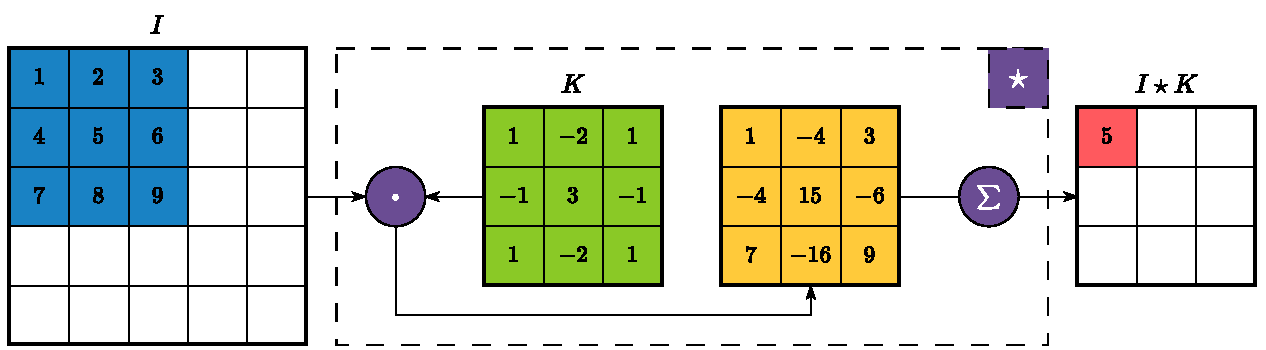
\includegraphics[width=\linewidth]{images/convolution.pdf}
    \caption[Convolution]{Convolution. Visualization of Equation~\eqref{e:cross_correlation}.}
    \label{fig:convolution}
\end{figure}
\newpage
In image processing, a convolution operation can involve more parameters than just the kernel itself. 
In this work, we will frequently refer to the following three:
\begin{description}
    \item[Stride.]
    Convolution operates by moving the kernel over the image.
    The size of each movement is called the stride.
    In PyTorch~\cite{PyTorchConv2d}, the default stride is 1.
    A commonly used choice is to set the stride equal to the kernel size.
    In this case, the kernel does not overlap between steps, and with a suitable kernel, this setup can be used to implement an average pooling layer (Section~\ref{sss:pooling}).
    In Figure~\ref{fig:dilate}, convolution with a stride set to 2 is shown.

    \begin{figure}
        \centering
        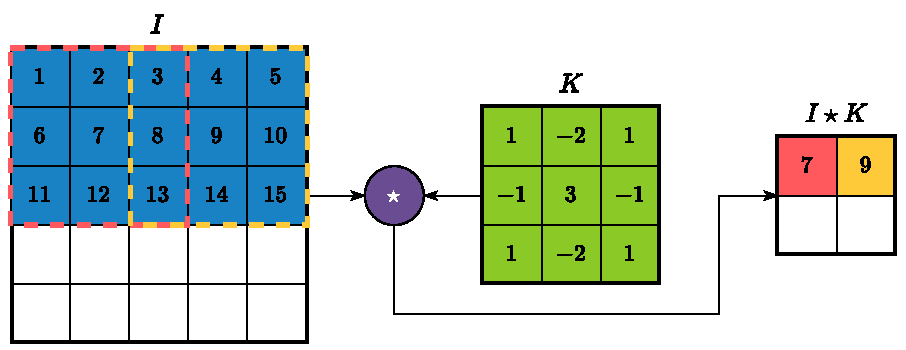
\includegraphics[width=0.75\linewidth]{images/stride.pdf}
        \caption[Stride]{Convolution with stride parameter 2.}
        \label{fig:stride}
    \end{figure}
    
    \item[Dilation.]
    In standard convolution, the kernel is applied to directly adjacent pixels in the image.
    This behavior can be altered by introducing the dilation parameter so that the kernel elements correspond to image pixels that are spaced apart rather than immediately neighboring.
    For a dilation parameter $d$, this is equivalent to convolving with a modified kernel $K'$, constructed by inserting $d-1$ zeros between consecutive values of $K$, as shown in Equation~\eqref{e:dilation}.
    In Figure~\ref{fig:dilate}, convolution with a dilation set to 2 is shown.

\NiceMatrixOptions{xdots/horizontal-labels}
\begin{equation}
    K'=
    \begin{bNiceArray}{ccccccccc}[first-row,last-col,margin]
        & \Hbrace{3}{d-1} \\
        K_{1,1} & 0 & \cdots & 0 & K_{1,2}  & 0 & \cdots & 0 & K_{1, n} \\
        0       &   &        &   &   0      &   &        &   & 0 & \Vbrace{3}{d-1} \\ 
        \vdots  &   & \ddots &   & \vdots   &   & \ddots &   & \vdots \\ 
        0       &   &        &   &   0      &   &        &   & 0 \\
        K_{2,1} & 0 & \cdots & 0 & K_{2,2}  & 0 & \cdots & 0 & K_{2, n} \\
        0       &   &        &   &   0      &   &        &   & 0 \\ 
        \vdots  &   & \ddots &   & \vdots   &   & \ddots &   & \vdots \\ 
        0       &   &        &   &   0      &   &        &   & 0 \\
        K_{m,1} & 0 & \cdots & 0 & K_{m,2}  & 0 & \cdots & 0 & K_{m, n} \\
    \end{bNiceArray}
    \label{e:dilation}
\end{equation}

\begin{figure}
    \centering
    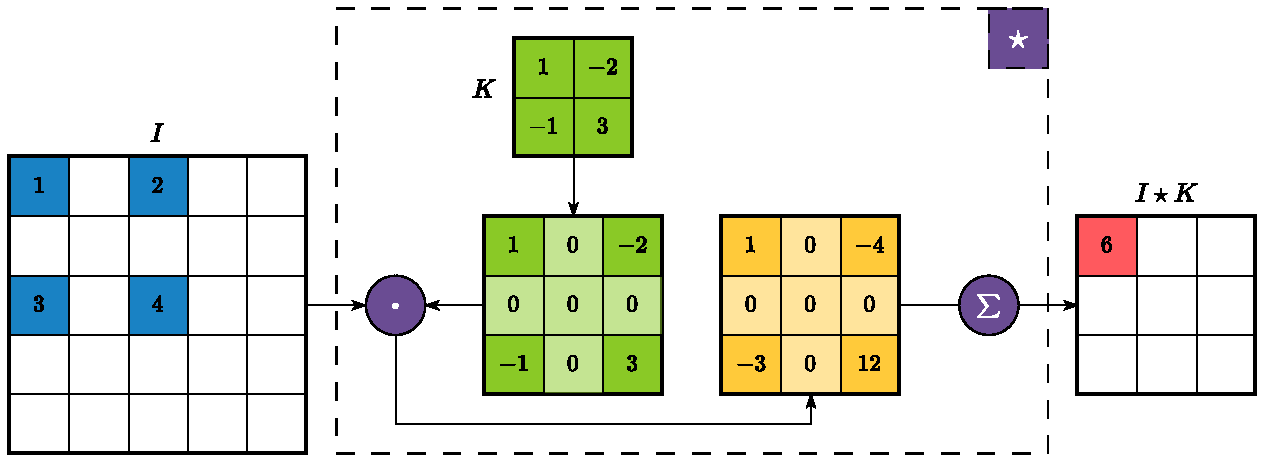
\includegraphics[width=\linewidth]{images/dilate.pdf}
    \caption[Dilation]{Convolution with dilation parameter 2.}
    \label{fig:dilate}
\end{figure}
    
    \item[Padding.]
    A standard convolution applied to an image of dimensions $n_1 \times n_2$ with a kernel of dimensions $k_1 \times k_2$ produces an output image of size $(n_1 - k_1 + 1) \times (n_2 - k_2 + 1)$.
    Thus, by default, the convolution operation decreases the spatial size of the input image.  
    To address this, padding is used.  
    Padding means adding extra rows and columns around the borders of the input image.  
    These added entries can be set to zero, copy the edge values, or even mirror the image content.
    The convolution is then performed on this padded image, and the resulting output can preserve the initial dimensions or even yield a larger image, though the latter is not commonly done.
    
\end{description}

\subsubsection{Pooling layers}
\label{sss:pooling}

Pooling layers closely resemble convolutional layers. 
They share the same core idea of moving a small window -- similar to a kernel -- across the image.
On the other hand, the difference is that these layers do not contain any learnable parameters, and the window usually moves with non-overlapping steps (stride of the window size).

Min-, max-, and average-pooling layers are types of pooling layers where, at each step, the minimum, maximum, or mean value within the window of the image is passed to the output image, respectively.
Furthermore, an average pooling layer with parameter $k$ can be interpreted as a convolution operation with a fixed (non-trainable) $k \times k$ kernel whose entries are all $k^{-2}$, applied with stride $k$.


\subsubsection{Activation function}

A common part of neural networks is the activation functions.
The most widely used activation function is ReLU (Equation~\eqref{e:relu}); however, other alternatives also exist (e.g. LeakyReLU Equation~\eqref{e:leaky_relu}).
These layers do not contain any trainable parameters.

\begin{align}
    \text{ReLU}(x) &\coloneqq \max(0, x) \label{e:relu} \\
    \text{LeakyReLU}(x) &\coloneqq 
        \begin{cases}
            0.01 x & x < 0 \\
            x & x \ge 0
        \end{cases}
        \label{e:leaky_relu}
\end{align}

\subsubsection{Pixel shuffle layer}

In order to perform downscaling, it is necessary to include a layer that increases the spatial resolution. 
One such layer is the pixel shuffle layer~\cite{Shi2016}, which transforms an input image with $C \cdot r^2$ channels and spatial size $H \times W$ into an output with $C$ channels and spatial dimensions $(H \cdot r) \times (W \cdot r)$ by rearranging the feature maps in the way that is illustrated in Figure~\ref{fig:pixel_shuffle}.
This layer has no trainable parameters, and both the values in the feature maps and the number of stored values remain unchanged.
The reverse operation, which takes $C$ channels of spatial size $(H \cdot r) \times (W \cdot r)$ and produces $C \cdot r^2$ channels of spatial size $H \times W$, is referred to as the \textit{pixel unshuffle layer}.

\begin{figure}
    \centering
    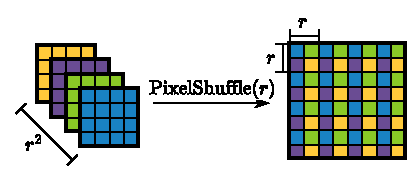
\includegraphics[width=0.5\linewidth]{images/pixel_shuffle.pdf}
    \caption[Pixel shuffle layer]{Pixel shuffle layer. Source: redesigned~\cite{Shi2016}.}
    \label{fig:pixel_shuffle}
\end{figure}
\newpage
\subsection{Evaluation metrics}

An essential part of machine learning is quantifying a model's performance.
Suppose we have a regression task. 
Let $\hat{Y} \in \mathbb{R}^{m, n}$ be the model output -- an image of dimension $m \times n$, and $Y \in \mathbb{R}^{m, n}$ be the target of the same dimension.
Evaluation metrics, therefore, express the difference between the target $Y$ and the model output $\hat{Y}$. 
There are endless possibilities to compare these two matrices; however, only a few are frequently used, such as Mean Square Error (MSE, Equation~\eqref{e:mse}), Mean Absolute Error (MAE, Equation~\eqref{e:mae}), and Root Mean Square Error (RMSE, Equation~\eqref{e:rmse}).
When the objects $Y$ and $\hat{Y}$ are images, these metrics are often referred to as pixel-wise evaluation metrics.

% Tu nie je \begin{equation}, je to problem??
\begin{align}
    \text{MSE}\left(Y, \hat{Y}\right) &\coloneqq \frac{1}{mn} \sum_{i=1}^m \sum_{j=1}^n \left( \hat{Y}_{i,j} - Y_{i,j} \right)^2 \label{e:mse} \\
    \text{MAE}\left(Y, \hat{Y}\right) &\coloneqq \frac{1}{mn} \sum_{i=1}^m \sum_{j=1}^n \left| \hat{Y}_{i,j} - Y_{i,j} \right| \label{e:mae} \\
    \text{RMSE}\left(Y, \hat{Y}\right) &\coloneqq \sqrt{\text{MSE}\left(Y, \hat{Y}\right)} \label{e:rmse}
\end{align}

\subsection{Optimizer}

The optimizer governs how a neural network is trained.
It determines how the model’s weights are updated and how it responds to improvements or declines in performance.
After each step, the gradient of the loss function is computed, and the optimizer uses this information to modify the weights of the layers.
This gradient exists because the loss function and the layers are differentiable.
There exist several algorithms suitable for this setting; however, throughout this work we will employ \textit{Adam}, whose detailed description can be found in~\cite{Kingma2017}.

\subsection{EDSR}

Various architectures are used for the purpose of downscaling in~\cite{Yang2024, Kostal2025, Vandal2017, Groenke2020, Rampal2025}, including Super-Resolution Convolutional Neural Network (SRCNN)~\cite{Dong2015}, Enhanced Deep Super-Resolution Network (EDSR)~\cite{Lim2017}, Normalizing Flows~\cite{Rezende2015}, Fourier Neural Operator (FNO)~\cite{Li2021}, Generative Adversarial Network (GAN)~\cite{Goodfellow2016}, and SwinIR~\cite{Liang2021}.

We will use the same architecture as Košťál et al.~\cite{Kostal2025}, where the EDSR model had a negligible performance difference from the best SwinIR model, although it is a simpler model.
In line with Lim et al.~\cite{Lim2017}, we use the L1 loss (MAE, Equation~\eqref{e:mae}) as the pixel-wise loss function throughout this work, instead of the L2 loss (MSE, Equation~\eqref{e:mse}), since it ``provides better convergence''.

EDSR is a neural network architecture designed by Lim et al.~\cite{Lim2017} specifically for SISR tasks.
Two main parameters influencing the size -- the number of parameters -- of EDSR are the number of residual blocks (\textit{res\_blocks}) and the number of channels (\textit{n\_features}) used within the model.
The whole architecture (Figure~\ref{fig:edsr}) can be divided into head, body, and tail parts.

The head consists of a convolutional layer, which takes the same number of channels as the input channel has and outputs \textit{n\_features} channels.
It is followed by the body, which is made of \textit{res\_blocks} residual blocks and one additional convolutional layer.
EDSR's residual blocks (Figure~\ref{sf:res_block}) were created by removing the batch normalization layers from ResNet's residual blocks~\cite{Lim2017}.
Therefore, EDSR has residual blocks containing two convolutional layers and a ReLU layer in between them; moreover, the residue is scaled by $0.1$ to stabilize the learning process~\cite{Lim2017}.
The body is connected to the head in a residual connection manner (Figure~\ref{sf:edsr}).
Finally, the tail involves an upsampler and a final convolutional layer, which yields the downscaled image with the same number of channels as the input.
The upsampler (Figure~\ref{sf:upsampler}) is made of pairs of convolutional and pixel shuffle layers for each prime factor of the scale factor.
The role of the convolutional layer is to produce $p_i^2 \cdot \textit{n\_features}$ channels, so that after applying the pixel shuffle layer with parameter $p_i$, the number of channels is returned to \textit{n\_features}.

\begin{figure}[h]
    \begin{subfigure}{0.25\linewidth}
        \centering
        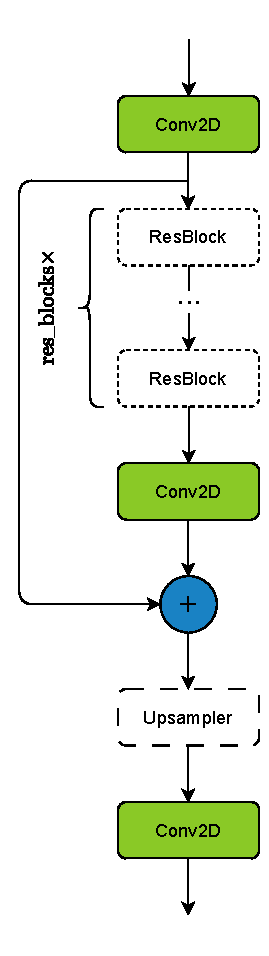
\includegraphics[width=\linewidth]{images/edsr.pdf}
        \caption{EDSR model}
        \label{sf:edsr}
    \end{subfigure}
    \begin{subfigure}{0.22\linewidth}
        \centering
        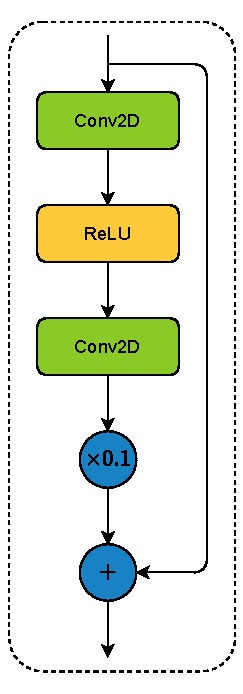
\includegraphics[width=\linewidth]{images/res_block.pdf}
        \caption{Residual block}
        \label{sf:res_block}
    \end{subfigure}
    \begin{subfigure}{0.48\linewidth}
        \centering
        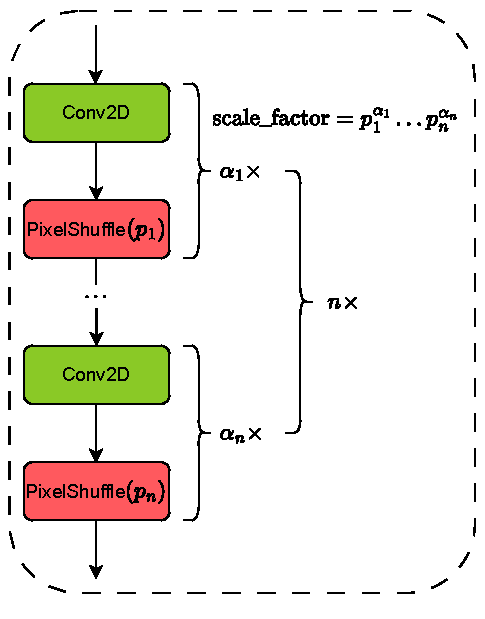
\includegraphics[width=\linewidth]{images/upsampler.pdf}
        \caption{Upsampler}
        \label{sf:upsampler}
    \end{subfigure}
    \caption[EDSR model architecture]{EDSR model architecture with detailed residual block and upsampler architectures. Note that in upsampler, the equation represents the factorization of scale\_factor, therefore $p_i$ are prime numbers. Source: redesigned visualization from Lim et al.~\cite{Lim2017}.}
    \label{fig:edsr}
\end{figure}

\section{Image processing}

Throughout this study, we will treat the climate variables as images, following a SISR-based approach.
Thus, image processing is a fundamental part of this approach used for downscaling; however, since it being a wide field of study, we will include only the necessary techniques used in this work.

We will use the definition of an image by Petrou M. M. P. and Petrou C.~\cite{Petrou2010}.
First, we will define the two-dimensional image function as $f:\mathbb{R} \times \mathbb{R} \to \mathbb{R}$.
The formula of the image function is usually unknown.
Therefore, as an image, we consider a grid sampling of the image function $f$, a real matrix $I \in \mathbb{R}^{m,n}$ having elements $I_{i,j} = f(i,j),\ i \in \{1, 2, \dots m\},\ j \in \{1, 2, \dots n\}$, usually referred to as pixels.

\subsection{Image derivative and gradient}

In this section, we introduced the image function, so it is natural to now discuss its derivatives.
As the image function has a two-dimensional domain, partial derivatives with respect to $x$ (horizontal) and $y$ (vertical) are considered.
Analogous to the image function, the formulas of $\frac{\partial}{\partial x}f$ and $\frac{\partial}{\partial y}f$ are not known in explicit form.
However, the sampled grid is known, and that allows us to make estimates for both partial derivatives.
A straightforward estimate of $\frac{\partial}{\partial x}f$, resp. $\frac{\partial}{\partial y}f$ are differences between neighboring pixels in columns, resp. rows:
\begin{equation}
\begin{aligned}
    \frac{\partial}{\partial x}f(i,j) &\approx I(i,j) - I(i,j+1), \\
    \frac{\partial}{\partial y}f(i,j) &\approx I(i,j) - I(i+1,j)
\end{aligned}
\label{e:simple_derivatives}
\end{equation}
These partial derivatives are also images of dimensions similar to $I$, except for one row and one column, respectively.
The Equations~\eqref{e:simple_derivatives} are implemented as convolutions of image $I$ with the following kernels:
\begin{equation}
K_x = \begin{bmatrix}1 & -1\end{bmatrix}, \qquad K_y = \begin{bmatrix}1 \\ -1\end{bmatrix}.
\label{e:simple_derivative_kernels}
\end{equation}
Therefore, the estimate is made by:
\begin{equation}
    \frac{\partial}{\partial x}f \approx K_x \star I, \qquad
    \frac{\partial}{\partial y}f \approx K_y \star I.
    \label{e:trivial_derivative_kernels}
\end{equation}
There are more possibilities for the choice of kernel.
The most common ones, however, include larger neighborhoods than the kernels in Equation~\eqref{e:simple_derivative_kernels}.
One of the most common choices is Sobel kernels (Equation~\eqref{e:Sobel_kernels}), which include $3\times3$ neighborhood, but the emphasis is on the neighbors that are on the same horizontal, respectively vertical line.
In Figure~\ref{fig:derivatives}, Sobel kernels were used to compute the derivatives with respect to both $x$ and $y$ of an image of a skyscraper.
It is evident that the edges perpendicular to the derivative direction are highlighted.

\begin{equation}
K_x = \begin{bmatrix}1 & 0 & -1 \\ 2 & 0 & -2 \\ 1 & 0 & -1\end{bmatrix}, \qquad K_y = \begin{bmatrix}1 & 2 & 1 \\ 0 & 0 & 0 \\ -1 & -2 & -1 \end{bmatrix}
\label{e:Sobel_kernels}
\end{equation}

\begin{figure}
    \centering
    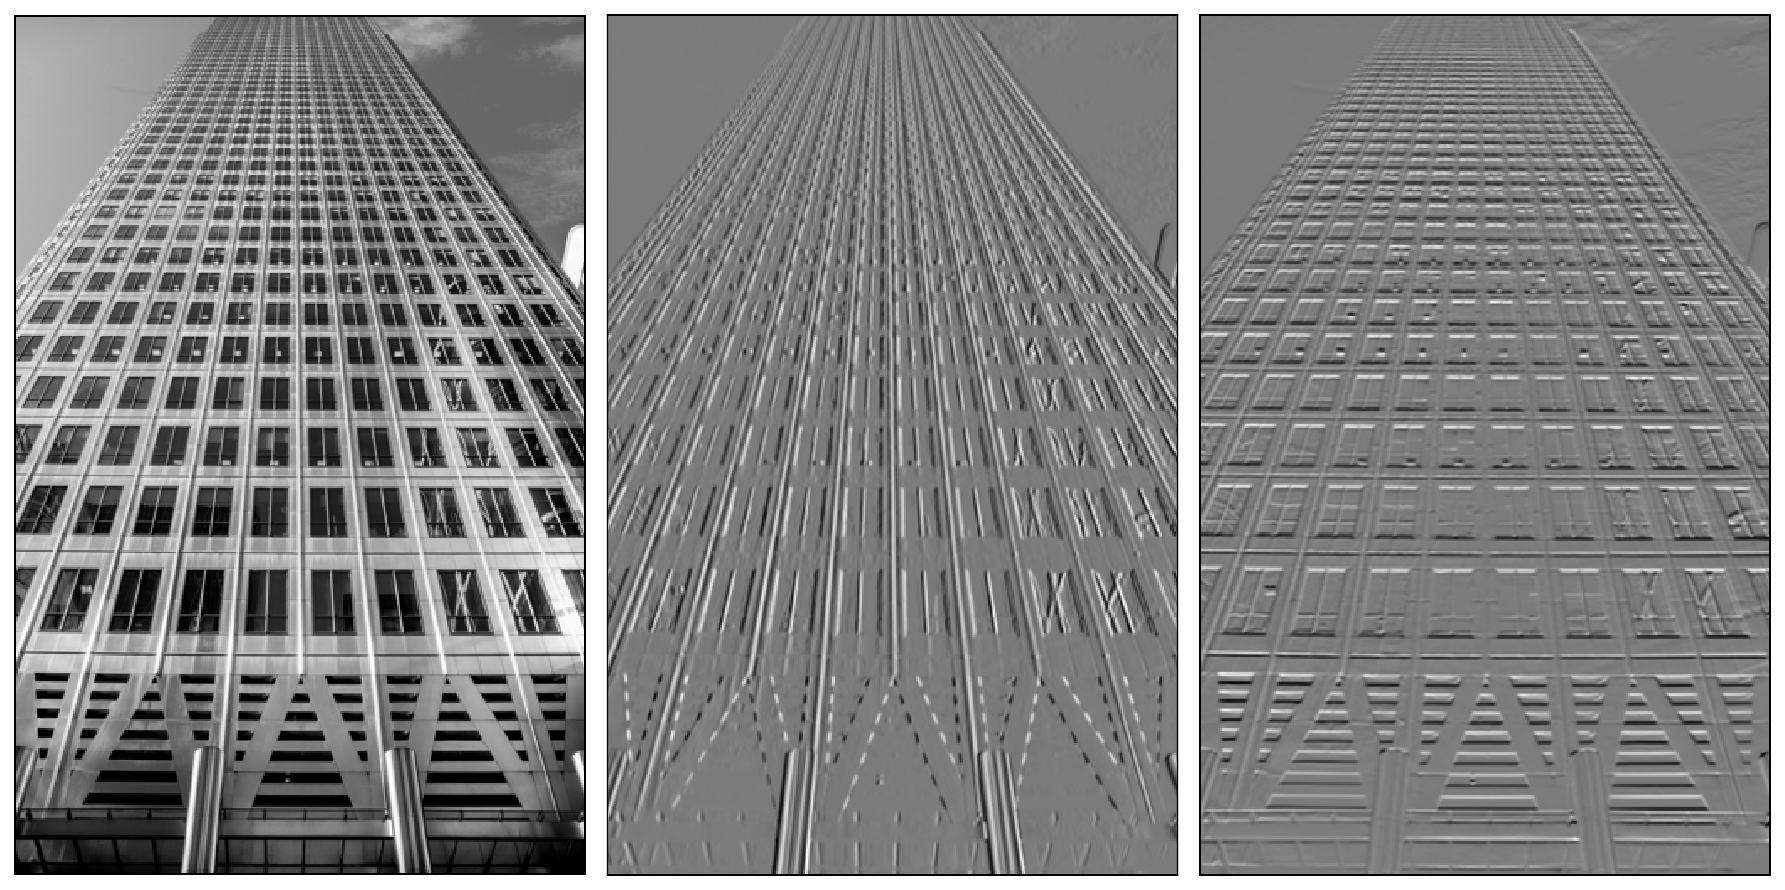
\includegraphics[width=\linewidth]{images/derivatives.pdf}
    \caption[Image derivatives]{Image derivatives. From left to right, the images represent the original image, its derivative with respect to $x$ (horizontal direction) and its derivative with respect to $y$ (vertical direction). In each of the derivative images, only the edges that are perpendicular to the direction of differentiation are visible, as expected. Source: Urban100~\cite{Huang2015}.}
    \label{fig:derivatives}
\end{figure}

Suppose we have now chosen the estimates $\frac{\partial}{\partial x}f$ and $\frac{\partial}{\partial x}f$.
Analogously to the common function, we define the image gradient (more accurately -- its estimate) as:
\begin{equation}
    \nabla f = \left( \frac{\partial}{\partial x}f, \frac{\partial}{\partial y}f \right)
\end{equation}
Thus, $\nabla f$ constitutes a particular kind of vector field (defined in Section~\ref{sss:vector_field}) known as a \textit{gradient vector field}.
Such a vector field is visualized in Figure~\ref{fig:climate_gradient} on real mean temperature data from ReKIS.
The image gradient, same as the conventional gradient, points to the direction of the biggest increase.

It is worth mentioning that the gradient usually does not point exactly to a single pixel; instead, it typically points between two pixels.
In the literature, the magnitude of this field (Equation~\eqref{e:gradient_magnitude}) is often referred to as the image gradient; nevertheless, we will treat these as distinct concepts.
In this work, we will abbreviate the approximation of the derivative of $f$ with respect to $x$ or $y$, computed from the values of the grid sampling $I$, by $\frac{\partial}{\partial x}I$ and $\frac{\partial}{\partial y}I$, respectively.
In the same manner, we will treat the estimate of the gradient of $f$ and denote it as $\nabla I$.

\begin{figure}
    \centering
    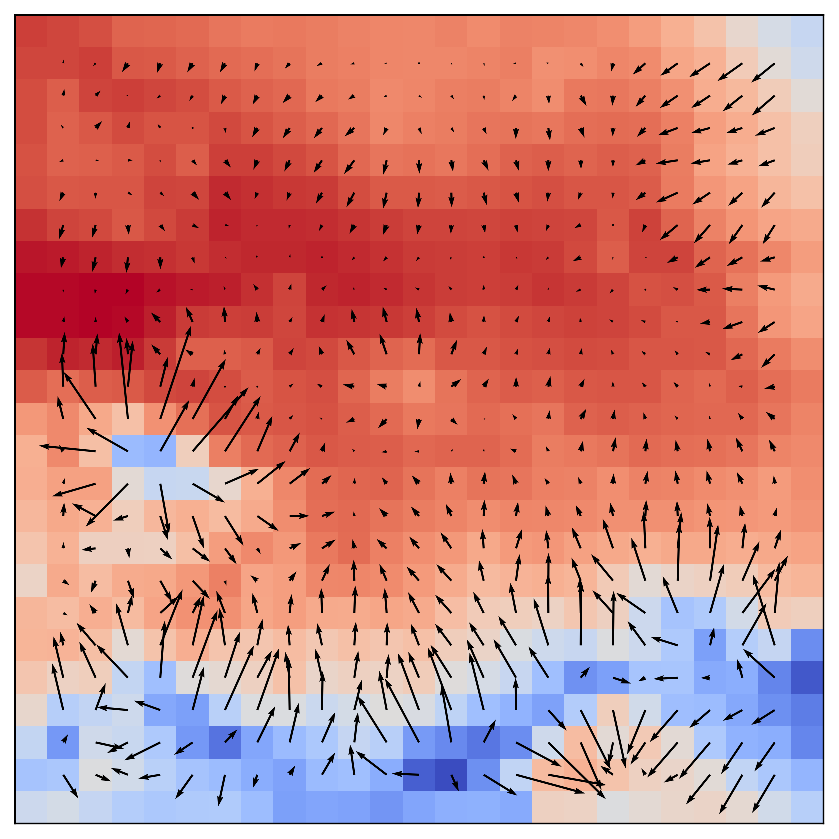
\includegraphics[width=0.5\linewidth]{images/climate_gradient.pdf}
    \caption[Image gradient]{Image gradient. Upscaled mean temperature data from ReKIS on 2000-02-01 is shown, with its gradient on top of that. As with a conventional gradient, the image gradient indicates the direction of the greatest increase in intensity.}
    \label{fig:climate_gradient}
\end{figure}

\begin{equation}
    M = \sqrt{\left( \frac{\partial}{\partial x}f\right)^2 + \left(\frac{\partial}{\partial y}f \right)^2 }
    \label{e:gradient_magnitude}
\end{equation}

\subsubsection{Vector field}
\label{sss:vector_field}

The general vector field is defined by Galbis and Maestre~\cite{Galbis2012} as a mapping that takes $n$-dimensional vectors into other $n$-dimensional vectors (Equation~\eqref{e:vector_field}).
\begin{equation}
    \mathbf{F}: U \subset \mathbb{R}^n \to \mathbb{R}^n
    \label{e:vector_field}
\end{equation}
In this work, only 2D vector fields will be used.
A vector field $\mathbf{F}$ can be represented by plotting the vectors $\mathbf{F}(\mathbf{x})$ on a grid, with each vector anchored at the point $\mathbf{x}$ (Figure~\ref{fig:climate_gradient}).
For a differentiable function $f\colon\mathbb{R}^n \to \mathbb{R}$, the mapping $\nabla f\colon\mathbb{R}^n\to\mathbb{R}^n$ defined as $\nabla f(\mathbf{x}) = \left( \frac{\partial}{\partial x_1}f(\mathbf{x}), \dots, \frac{\partial}{\partial x_n}f(\mathbf{x}) \right)$, referred to as the gradient, is a special type of vector field. 
The gradient vector field indicates, at every point in the domain of $f$, the direction of steepest increase.

\begin{figure}
    \centering
    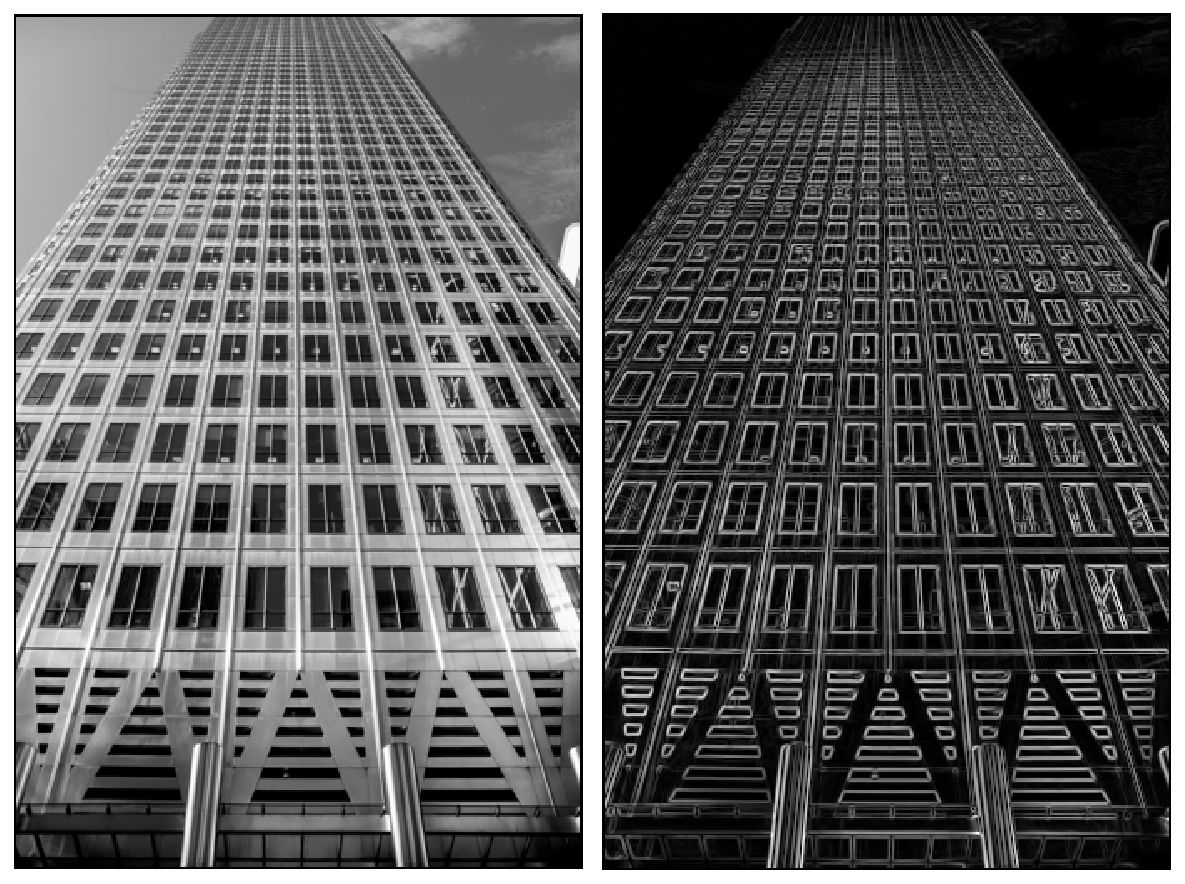
\includegraphics[width=0.66\linewidth]{images/gradient_magnitude.pdf}
    \caption[Image gradient magnitude]{Image gradient magnitude. From the derivatives in Figure~\ref{fig:derivatives} of the original image (left), image gradient magnitude (right) was calculated using Equation~\eqref{e:gradient_magnitude}. As expected, the gradient magnitude is the highest on the edges of the image and is almost zero on the same intensity regions. Source: Urban100~\cite{Huang2015}.}
    \label{fig:placeholder}
\end{figure}

\subsubsection{Dilated derivative}
\label{ss:dilated_sr_derivative}

The purpose of introducing the dilated derivative is its consistency throughout the downscaling process, which will be derived here.
Suppose we are given a high-resolution image $I^\text{HR}$, and we apply a resampling procedure -- implemented as a convolution with a kernel -- to decrease its resolution by a factor of $s$ (such as the average pooling).
For the sake of clarity, we define the downsampling operator on 2D images.

\begin{definition}[Downsampling operator]
Let $I \in \mathbb{R}^{m,n}$, $m,n\in\mathbb{N}$ be a real matrix.
For any $s \in \mathbb{N}$ such that $s \le \min(m,n)$, we define the downsampling operator $\downarrow_s$, which decreases the resolution of $I$ by a factor of $s$, as:
$$(I{\downarrow_s})[i,j] = I[is, js].$$
The output $I{\downarrow_s}$ is of dimensions $\lfloor\frac{m}{s}\rfloor \times \lfloor\frac{n}{s}\rfloor$.
\label{d:downsampling_operator}
\end{definition}
Using the downsampling operator defined in Definition~\ref{d:downsampling_operator}, the LR images can be obtained from HR images the following way:
\begin{equation}
I^\text{LR} = \left(I^\text{HR} \star k_R\right)\downarrow_s,     
\end{equation}
where $\star$ denotes the convolutional operator and $k_R$ denotes the resampling kernel of dimensions $s\times s$, for example, the average pooling kernel, filled with $s^{-2}$.
\begin{lemma}[Noble identity]
Let $I \in \mathbb{R}^{m_1,n_1}$, $m_1,n_1\in\mathbb{N}$ be a real matrix, $k \in \mathbb{R}^{m_2, n_2}$ be a real kernel, and $s\in \mathbb{N}$ be a downsampling factor.
Then the following equation holds true:
$$I{\downarrow_s}\star k = \left(I \star k^{(s)}\right){\downarrow_s},$$
where $k^{(s)}$ is a dilated kernel by $s$, meaning that between the elements of kernel $k$, $s-1$ zeros were added. 
This equation holds true only when both sides of the equation are well-defined.
\cite{Smith2011}
\label{l:noble_identity}
\end{lemma}
Lemma~\ref{l:noble_identity} will be particularly useful when $k$ is a derivative kernel $k_x$, such that $I \star k_x = \frac{\partial}{\partial x} I$; then:
\begin{equation}
\frac{\partial}{\partial x} I^\text{LR} = I^\text{LR} \star k_x = \left(I^\text{HR} \star k_R \right){\downarrow_s} \star k_x = \left(I^\text{HR} \star k^{(s)}_x \star k_R\right){\downarrow_s} = \partial_x^sI^\text{HR}.
\label{e:mean_sr_derivative}
\end{equation}
Thus, in this work, we will refer to $\partial_x^sI^\text{HR}$ as the dilated derivative by factor $s$ of $I^\text{HR}$ with respect to $x$.
The interpretation of Equation~\eqref{e:mean_sr_derivative} is that a derivative in a particular direction of a LR image is the same as the derivative in the distance of the downsampling factor of the HR image convolved with the resampling kernel and downsampled.
This allows us to enforce this relationship when downscaling between LR input and SR model output.
Furthermore, this approach is valid when applied to the gradient vector field of $I^\text{LR}$:
\begin{equation}
\begin{aligned}
    \nabla I^\text{LR} &= \left(\frac{\partial}{\partial x} I^\text{LR}, \frac{\partial}{\partial y} I^\text{LR}\right) \\
    &= \left(\partial_x^sI^\text{HR}, \partial_y^sI^\text{HR}\right).
\end{aligned}
\end{equation}

\section{Constraints}
\label{s:physical_constraints}

Some previous studies overlook that the variable being downscaled represents a physical quantity and therefore must comply with the underlying physical laws~\cite{Beucler2021}. 
The main objective, minimizing a standard pixel-wise metric (e.g., MSE, RMSE, MAE), becomes an obstacle for the model to learn physical relations, which instead produces physically inconsistent outputs only to avoid penalty~\cite{Beucler2021}. 
Therefore, if we want to improve physical consistency, we need either to penalize the physical violations or completely forbid such behavior.
Both of these strategies can be viewed as \textit{constraints}, and frameworks for their implementation have been presented by Harder et al.~\cite{Harder2023} and Beucler et al.~\cite{Beucler2021}.
In both of these works, these techniques not only lead to physically (more) consistent outputs, but the incorporation of appropriate physical constraints has exerted a demonstrably positive effect on model accuracy.

Neural networks perform mapping from the input space to the output space.
The purpose of all machine learning models is for the output to be as close to the correct solution as possible.
In the case of downscaling, the output space has a significantly higher dimension than the input space.
This provides the model with an extensive space to find the correct solution.
However, this space contains subspaces that are highly improbable or entirely impossible to contain the solution.
Temperature positivity in Kelvins is a straightforward example.
Moreover, according to the manifold hypothesis, if we pick a random point in that space, we certainly would not be close to one of the solutions, which leads us to the conclusion that the solutions are not uniformly distributed throughout the output space~\cite{Goodfellow2016}.
In conclusion, the practice of assigning a penalty to a model when its output far from our prior knowledge is known as \textit{soft-constraining}, while restricting the set of possible outputs to a particular subspace is known as \textit{hard-constraining}.

\subsection{Definition of constraints}
\label{ss:constraining}
Let $\mathbf{f}\colon \mathbb{R}^n \to \mathbb{R}^m$ be a neural network performing downscaling.
Furthermore, let $(g,h), g\colon\mathbb{R}^n \to \mathbb{R}^k, h\colon \mathbb{R}^m \to \mathbb{R}^k$ be a pair of arbitrary functions.
In these functions, it is possible to specify the constraining logic.
Then, the violation of a particular constraint is for the input LR image $I^{\text{LR}} \in \mathbb{R}^n$ and the output SR image $\mathbf{f}\left(I^{\text{LR}}\right) = I^{\text{SR}} \in \mathbb{R}^m$:
\begin{equation}
    \mathcal{L}_c = l\left(g\left(I^{\text{LR}}\right), h\left(I^{\text{SR}}\right)\right),
    \label{e:constraint}
\end{equation}
where $l$ is an evaluation metric (e.g. MAE). 

Additional definitions of constraining exist (Harder et al.~\cite{Harder2023}, Beucler et al.~\cite{Beucler2021}), but they are overly restrictive, primarily because they also prescribe a specific implementation framework.
Although those definitions are not equivalent, both agree that a constraint is a relationship between model input and output, excluding the target.

\subsection{Soft constraints}
\label{ss:soft}

Soft constraints do not directly restrict the output space.
Instead, they introduce a penalty if the output is far from our prior knowledge.
This approach is equivalent to minimizing the constraint violation $\mathcal{L}_c$ in Equation~\eqref{e:constraint}.
Training a model is minimizing its loss function; therefore, it is straightforward that soft constraints will be implemented as the loss function, representing the constraint violation itself.
Typically, $\mathcal{L}_c$ does not constitute the entire loss function; rather, it is used in conjunction with a conventional pixel-wise evaluation metric $\mathcal{L}_p$. 
Accordingly, the overall loss function $\mathcal{L}$ for a soft-constrained model is:
\begin{equation}
    \mathcal{L} = (1 - \alpha) \mathcal{L}_p + \alpha \mathcal{L}_c,
    \label{e:soft_constraint}
\end{equation}
where $\alpha \in [0, 1]$ controls the intensity of the constraint.
Every constraint matching the form in Equation~\eqref{e:constraint} can be implemented as a soft constraint in this manner.

Various works include a physically inspired modification of the loss function~\cite{Lu2019, Ge2023, Xiong2025}.
However, most of them are only loss functions -- quantifying the difference between model output (SR image) and the HR target image.
We gathered several of these methods that depend on image derivatives or gradients
and adapted them using the principle of derivative conservation under downscaling (Section~\ref{ss:dilated_sr_derivative}), enabling their use as soft constraints.

\subsubsection{Conservation law}
\label{sss:soft_conservation}

Harder et al.~\cite{Harder2023} used the mass conservation law in downscaling the column integrated water content. 
The conservation law implies that, during the downscaling process, mass or energy can neither be lost nor generated.
Thus, the goal of a soft constraint of the conservation law is to minimize the difference between the LR pixel value and the mean integrated water content of the corresponding SR pixels.
One of the experiments in~\cite{Harder2023} was to preserve column-integrated moist static energy through downscaling the same quantity along with water content and water vapor.
From these quantities, the mean temperature was calculated.
Another experiments from~\cite{Harder2023} were to apply the conservation law purely to the mean temperature, which does not have a physical background.
However, in one experiment employing this configuration, an improvement was observed relative to the baseline model.
In this work, we will focus solely on the mean temperature; therefore, the conservation law in this work will be used in a similar vein as in~\cite{Harder2023}.

Suppose that we have a LR image $I^\text{LR} \in \mathbb{R}^{n,n}$ and its $i$-th pixel $I^\text{LR}_i$.
Let $\left\{I^\text{SR}_{i, j} \mid j=1,\dots,s^2\right\}$ be the corresponding set of pixels downscaled from $I^\text{LR}_i$ by a scale factor $s$.
Then, the conservation law is defined by the equation:
\begin{equation}
    I^\text{LR}_i = \frac{1}{s^2}\sum_{j=1}^{s^2}I^\text{SR}_{i, j}
    \label{e:conservation}
\end{equation}
for each $i = 1, \dots, n$. 
In summary, the conservation law entails preserving a physical quantity, such as mass or energy, so that the mean value of the downscaled pixels remains equal to that of the corresponding original LR pixel.
Naturally, in soft constraining, the error between the two sides of Equation~\eqref{e:conservation} will be minimized.
We note that the right side of Equation~\eqref{e:conservation} is equivalent to average pooling with a kernel of size $s \times s$.
Therefore, we can denote the later average pooling output as $\bar{I}^\text{SR}$. 
The constraint violation is then:
\begin{equation}
    \mathcal{L}_c = l\left(I^\text{LR}_i, \bar{I}^\text{SR}\right),
\end{equation}
for an evaluation metric $l$ (MAE and MSE will be implemented and experimented with).

\subsubsection{Simple derivative constraint}

The derivative constraint, as its name suggests, is a very straightforward continuation of Section~\ref{ss:dilated_sr_derivative}.
The constraint builds upon the fact that both $I^\text{LR}$ partial derivatives $\frac{\partial}{\partial x}I^\text{LR}$ and $\frac{\partial}{\partial y}I^\text{LR}$ are the same as the dilated derivatives $\partial_x^sI^\text{HR}$ and $\partial_y^sI^\text{HR}$ of $I^\text{HR}$.
This suggests the penalization of this difference in the case of  $I^\text{SR}$.
So the constraint violation is:
\begin{equation}
    \mathcal{L}_c = l\left(\frac{\partial}{\partial x} I^\text{LR}, \partial^s_x I^\text{SR}\right) + l\left(\frac{\partial}{\partial y} I^\text{LR}, \partial^s_y I^\text{SR}\right),
\end{equation}
where $l$ is an evaluation metric; in this work, MAE and MSE will be used.
To obtain the derivatives with respect to $x$ and $y$, the convolution of the image with simple (Equation~\eqref{e:simple_derivative_kernels}) kernels will be used.

\subsubsection{Sobel gradient magnitude constraint}

Lu and Chen~\cite{Lu2019} improved an U-Net architecture for downscaling natural images by using an additional loss term -- gradient magnitude difference.
For pairs of $I^\text{SR}$ and $I^\text{HR}$, they calculated the image derivatives $\frac{\partial}{\partial x} I^\text{SR}$, $\frac{\partial}{\partial y} I^\text{SR}$, $\frac{\partial}{\partial x} I^\text{HR}$, and $\frac{\partial}{\partial y} I^\text{HR}$ using Sobel kernels.
Then, for both $I^\text{SR}$ and $I^\text{HR}$, they obtained gradient magnitudes $M^\text{SR}$ and $M^\text{HR}$ from the derivatives using Equation~\eqref{e:gradient_magnitude}. 
The loss function was the MSE between $I^\text{SR}$ and $I^\text{HR}$, and the MSE between the gradient magnitudes $M^\text{SR}$ and $M^\text{HR}$.
However, this is not a constraint as defined in Section~\ref{ss:constraining} because it also depends on the HR image.
Thus, the modification of this process is required.
This is done by computing the dilated SR derivatives Section~\ref{ss:dilated_sr_derivative} using Sobel kernels with respect to $x$ and $y$, resulting in $\partial^s_x I^\text{SR}, \partial^s_y I^\text{SR}$.
Again, the magnitude of the SR gradient is computed using the Equation~\eqref{e:gradient_magnitude}; however, in this case, the dilated SR derivatives are used:
\begin{equation}
    \bar{M}^{SR} = \sqrt{\left(\partial^s_x I^\text{SR}\right)^2 + \left(\partial^s_y I^\text{SR}\right)^2}.
\end{equation}
Therefore, the final soft constraining loss will be:
\begin{equation}
    \mathcal{L}_c = l\left(\bar{M}^\text{SR}, M^\text{LR}\right) 
\end{equation}
for a voluntary evaluation metric $l$.

\subsubsection{Temperature field continuity}

Xiong~\cite{Xiong2025} used a modified loss function for spatiotemporal downscaling of temperature near the Yangtze River.
In the work, the term temperature field continuity was used as the square of the difference between neighboring pixels in the horizontal and vertical directions.
This is equivalent to the square of a derivative computed by a trivial kernel (Equation~\eqref{e:trivial_derivative_kernels}).
Therefore, the used loss function can be described as:
\begin{equation}
    \begin{aligned}
        E_c &= \biggl|\sum\left(\frac{\partial}{\partial x} I^\text{SR}\right)^2 + \sum\left(\frac{\partial}{\partial y}I^\text{SR}\right)^2 \\
        &- \sum\left(\frac{\partial}{\partial x}I^\text{HR}\right)^2 - \sum\left(\frac{\partial}{\partial y}I^\text{HR}\right)^2\biggr|.
    \end{aligned}
    \label{e:xiong_continuity}
\end{equation}
However, Equation~\eqref{e:xiong_continuity} does not act as a constraint, since it also relies on HR images.
We adjust the loss function by removing $I^\text{HR}$, incorporating $I^\text{LR}$, and applying the dilated derivatives of $I^\text{SR}$ described in Section~\ref{ss:dilated_sr_derivative}. 
In addition, $E_c$ may grow excessively for large images or batch sizes; thus, we take the mean over pixels.
Equations~\eqref{e:continuity} show the modifications made to stabilize the loss function values and to comply with the soft constraining definition in the absolute, resp. square version.

\begin{equation}
    \begin{aligned}
    \mathcal{L}_c^\text{A} &= \frac{1}{N} \biggl|\sum\left|\partial^s_xI^\text{SR}\right| + \sum\left|\partial^s_yI^\text{SR}\right| \\
    &- \sum\left|\frac{\partial}{\partial x} I^\text{LR}\right| - \sum\left|\frac{\partial}{\partial y}I^\text{LR}\right|\biggr| \\
    \mathcal{L}_c^\text{S} &= \frac{1}{N}\biggl|\sum\left(\partial^s_x I^\text{SR}\right)^2 + \sum\left(\partial^s_y I^\text{SR}\right)^2 \\
    &- \sum\left(\frac{\partial}{\partial x}I^\text{LR}\right)^2 - \sum\left(\frac{\partial}{\partial y}I^\text{LR}\right)^2\biggr|
    \end{aligned}
    \label{e:continuity}
\end{equation}

\subsubsection{Gradient direction constraint}

Xiong~\cite{Xiong2025} inspired us to focus on the gradient directions, not only the magnitudes.
The above approaches depend on the derivatives or the magnitude of the gradient, not its orientation.
Xiong~\cite{Xiong2025} applied the \textit{atan2} function to pairs of horizontally and vertically adjacent pixels, summed these results, and then computed the difference between the SR output and the HR target, as shown in Equation~\eqref{e:xiong_dir_continuity}.
These values, however, did not correspond to any particular angles; they only captured global characteristics of the field.
\begin{equation}
    \begin{aligned}
        \mathcal{L}_d = \biggl| 
        \sum_{i = 1}^M\sum_{j = 1}^{N-1} \text{atan2}\left(I^\text{SR}_{i,j}, I^\text{SR}_{i,j + 1}\right) & +
        \sum_{i = 1}^{M - 1}\sum_{j = 1}^{N} \text{atan2}\left(I^\text{SR}_{i,j}, I^\text{SR}_{i+1,j}\right) \\ -
        \sum_{i = 1}^M\sum_{j = 1}^{N-1} \text{atan2}\left(I^\text{HR}_{i,j}, I^\text{HR}_{i,j + 1}\right) & -
        \sum_{i = 1}^{M - 1}\sum_{j = 1}^{N} \text{atan2}\left(I^\text{HR}_{i,j}, I^\text{HR}_{i+1,j}\right)
        \biggr|
    \end{aligned}
    \label{e:xiong_dir_continuity}
\end{equation}
However, the Equation~\eqref{e:xiong_dir_continuity} does not comply with the constraining setup.
It uses the HR target; instead, we will define it for LR input and dilated SR derivatives.
Furthermore, we will modify the function by incorporating local elements that are interpretable.
The key idea is to compare the orientations of the LR gradient and the dilated SR gradient vectors in each point of the image.
We will employ the cosine similarity function for this purpose, defined as:
\begin{equation}
    \text{cos\_sim}(u, v) = \frac{u \cdot v}{\|u\|\cdot\|v\|},
    \label{e:cos_sim}
\end{equation}
where $u,v$ are two dimensional vectors.
This function's range is $[-1, 1]$, when the direction of $u$ and $v$ is the same, resp. is perpendicular, resp. is exactly the opposite, their cosine similarity is equal to $1$, resp. $0$, resp. $-1$.
Therefore, we first calculate the dilated SR derivatives $\partial_x^s I^\text{SR}$, $\partial_y^s I^\text{SR}$ of the SR image with respect to $x$ and $y$.
If the $\partial_x^s I^\text{SR}$, $\partial_y^s I^\text{SR}$ are not the same shapes as a result of the derivative kernel choice, they need to be trimmed.
Then we can calculate the angle similarity matrix S as:
\begin{equation}
    \text{S} = 
    \text{cos\_sim}\left(\left(\partial^s_x I^\text{SR}, \partial^s_y I^\text{SR} \right), \left(\frac{\partial}{\partial x} I^\text{LR}, \frac{\partial}{\partial y} I^\text{LR}\right)\right),
\end{equation}
where the cos\_sim function is applied element-wise to matching indices in the matrices, resulting in a matrix.
Furthermore, we will scale the errors by the magnitude of the LR gradient (Equation~\eqref{e:magnitude}) in the corresponding point because we do not want to punish large angle differences in areas where the gradient magnitude is almost zero.
\begin{equation}
    \text{M} = \sqrt{\left(\frac{\partial}{\partial x} I^\text{LR}\right)^2 + \left(\frac{\partial}{\partial y} I^\text{LR}\right)^2}
\label{e:magnitude}
\end{equation}
Therefore, the final constraint violation will be:
\begin{equation}
    \begin{aligned}
        \mathcal{L}_c^\text{A} &= \frac{1}{mn}\sum_{i = 1}^m\sum_{j = 1}^n(1-S_{i,j})M_{i,j}, \\
        \mathcal{L}_c^\text{S} &= \frac{1}{mn}\sum_{i = 1}^m\sum_{j = 1}^n\left((1-S_{i,j})M_{i,j}\right)^2.
    \end{aligned}
\end{equation}

To obtain the derivatives with respect to $x$ and $y$, the convolution of the image with simple (Equation~\eqref{e:simple_derivative_kernels}), resp. Sobel (Equation~\eqref{e:Sobel_kernels}) kernels will be used; in that case, we will refer to this constraint as simple, resp. Sobel gradient direction constraint.

\subsubsection{G-Loss}

Ge and Dou~\cite{Ge2023} introduced a G-Loss loss function for downscaling natural images.
It belongs to other derivative-difference-based loss functions, as mentioned above.
However, its uniqueness is hidden in the usage of the derivatives in a distance $s$ in the HR image for downscaling with a downscaling factor $s$ and the derivatives being with respect to all 8 directions.
The loss is applied on HR and SR images. 
It consists of pixel-wise loss and a derivative-difference-inspired approach. 

When the downscaling is done with a scale factor of 1, only the derivatives are compared by L1-loss in addition to the direct L1-loss between the HR and SR images, as shown in Figure~\ref{fig:gloss}. 
However, when the scale factor is larger, average or max pooling can be applied to both HR and SR images, and afterward, the result is convolved with the derivative kernels.
The extracted patches from the LR and HR images are evaluated using an L1 loss between them.

Nevertheless, the results in~\cite{Ge2023} were the best when splitting (pixel shuffle) layers were used instead of average or max pooling layers.
The interpretation of the latter approach is that the derivative kernels are applied to the neighboring pixels in the split patches; however, those are in a distance of the scale factor $s$ in the original image, as visible in Figure~\ref{fig:mean_sr_gradient}.
Moreover, the process of convolving the split patches with derivative kernels is equivalent to performing a dilated convolution on the original images.
Therefore, if we pick one particular derivative kernel, convolve the split patches by it, and calculate the mean across the resulting patches, we obtain the dilated derivative. 
Thus, to convert this loss function -- more precisely, the part containing the splitting and derivative computation -- into a soft constraint, we use the dilated derivatives of $I^\text{SR}$ and compare them with the derivatives of $I^\text{LR}$.

\begin{figure}[htbp]
    \centering
    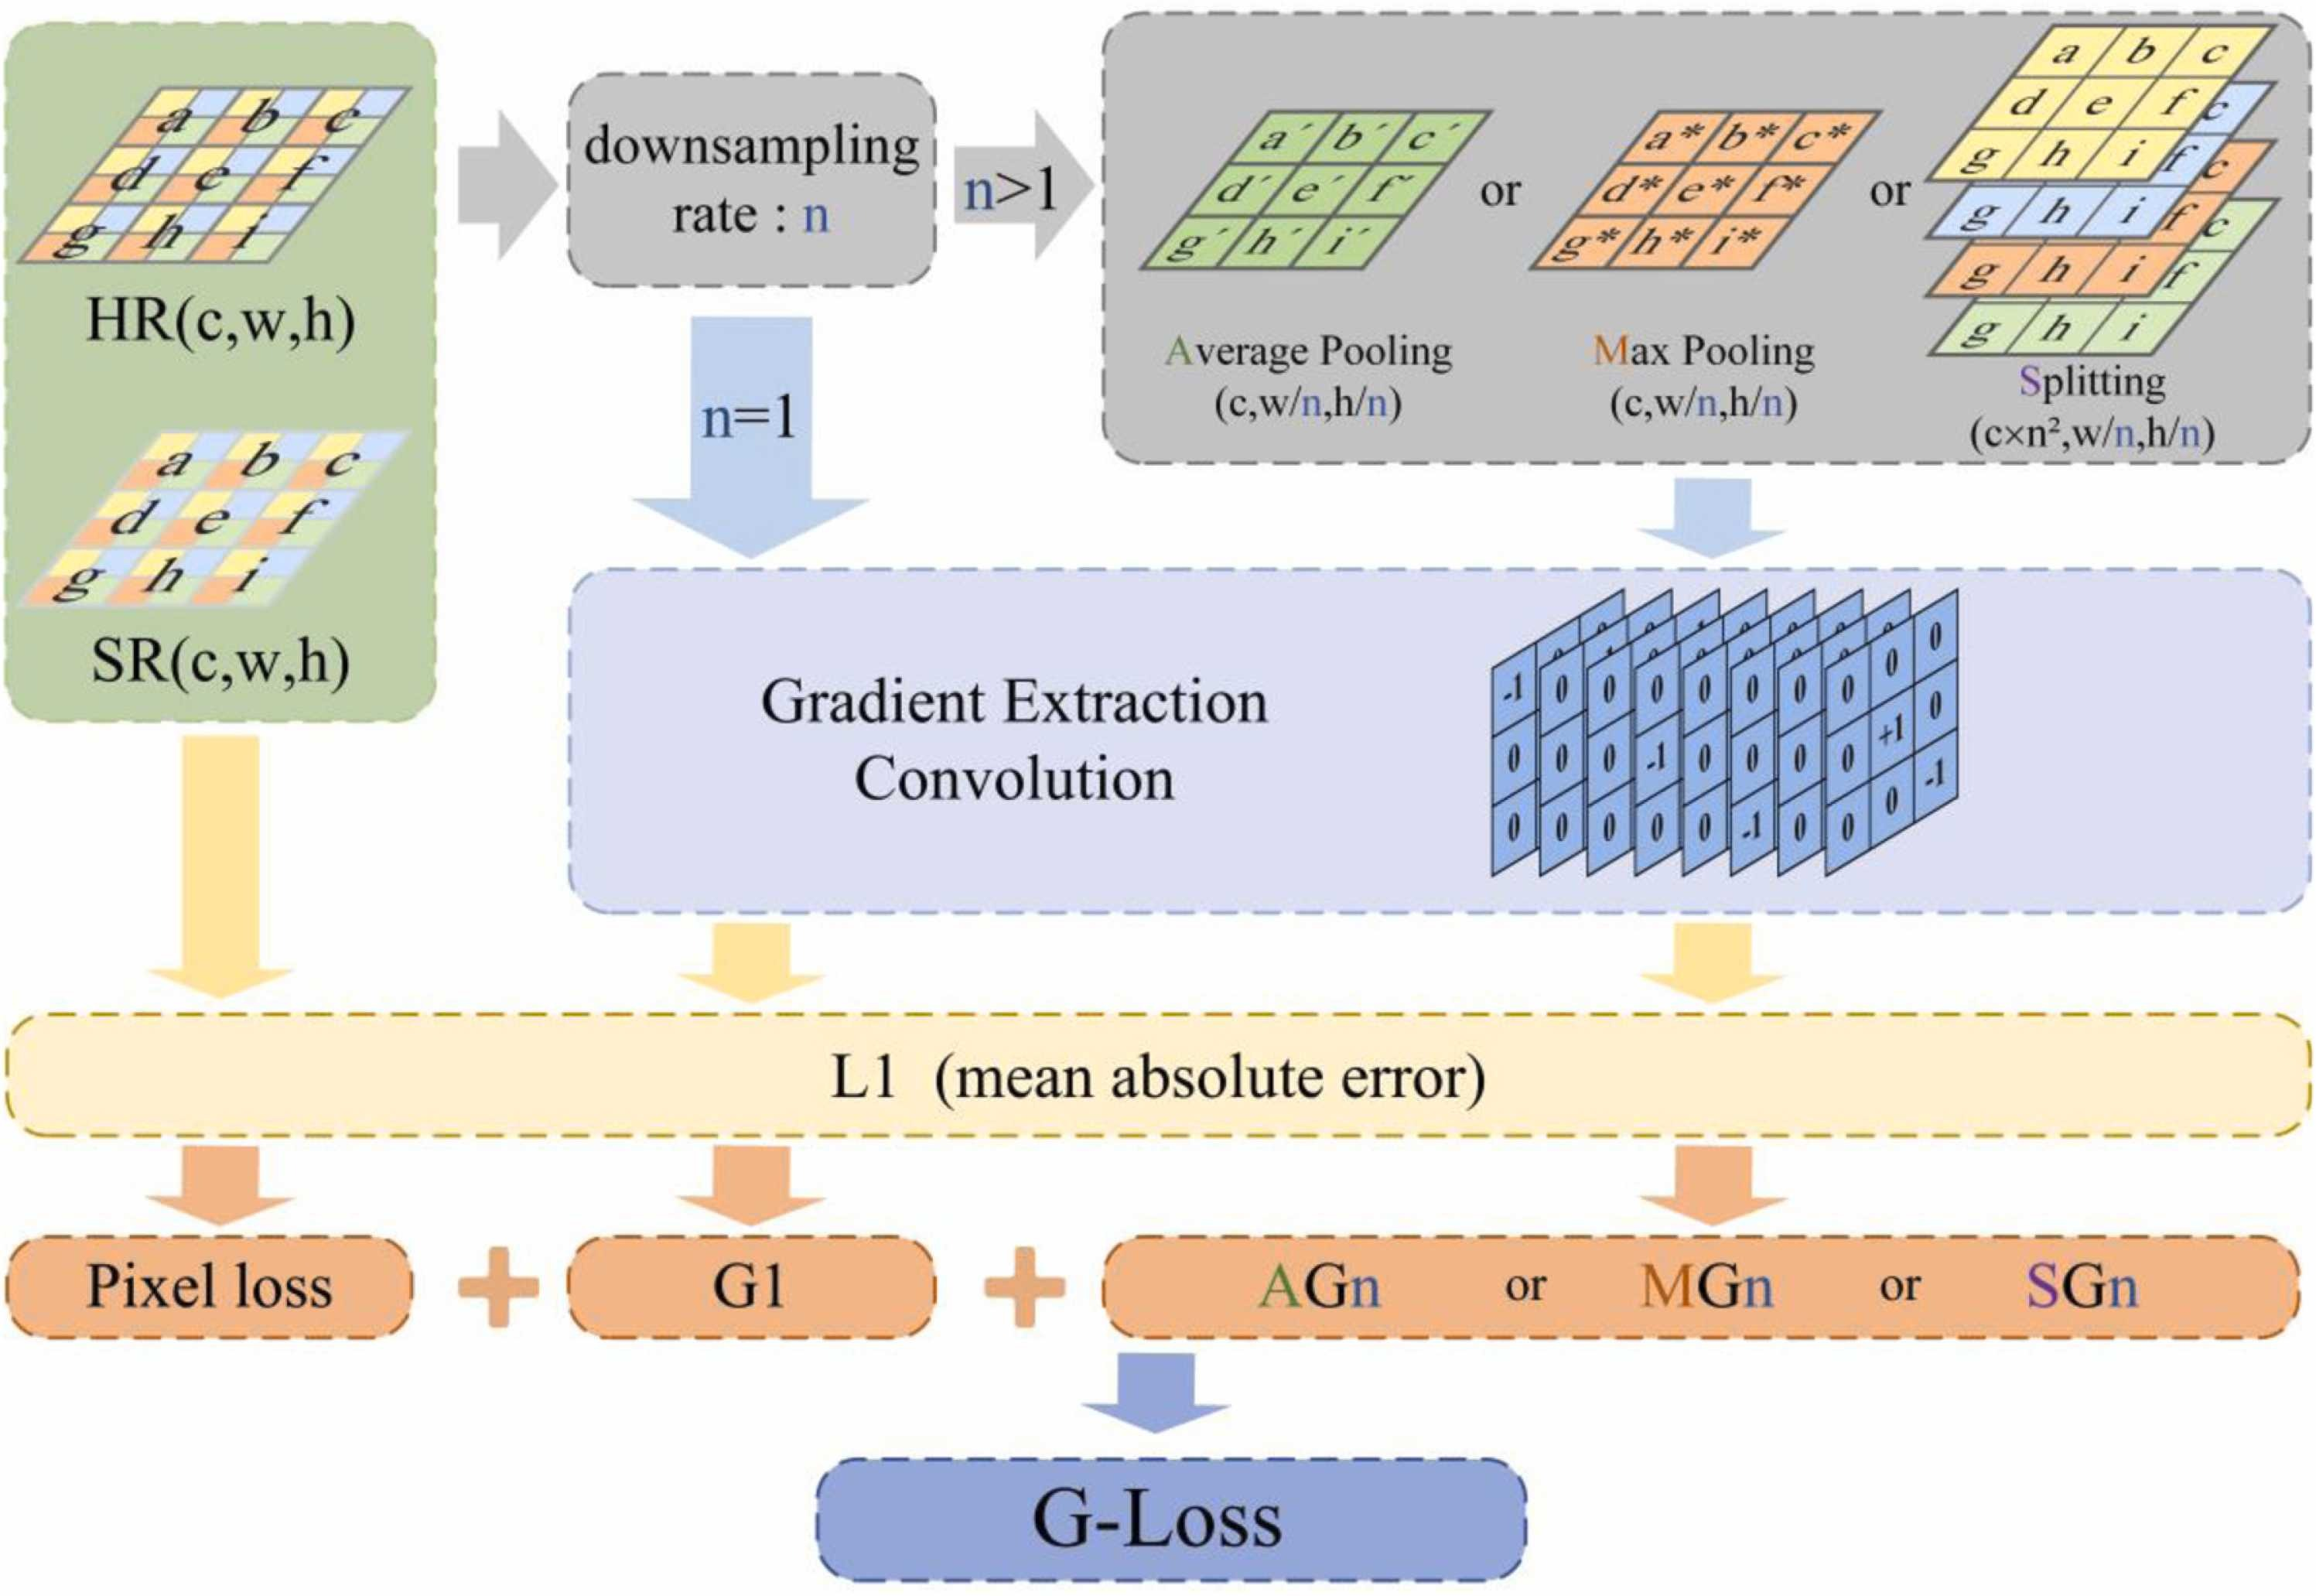
\includegraphics[width=0.8\linewidth]{images/gloss.jpg}
    \caption[G-Loss]{G-Loss. Source: Ge and Dou~\cite{Ge2023}.}
    \label{fig:gloss}
\end{figure}

The constraint violation is dependent on the derivatives in all eight directions.
They will be calculated using the kernels in Equation~\eqref{e:direction_kernels}.
\begin{equation}
    \begin{aligned}
        K = \Biggl\{ 
            &\begin{bmatrix} -1 & 0 & 0 \\ 0 & 1 & 0 \\ 0 & 0 & 0 \end{bmatrix},
            \begin{bmatrix}  0 & -1 & 0 \\ 0 & 1 & 0 \\ 0 & 0 & 0 \end{bmatrix},
            \begin{bmatrix}  0 & 0 & -1 \\ 0 & 1 & 0 \\ 0 & 0 & 0 \end{bmatrix},
            \begin{bmatrix}  0 & 0 & 0 \\ -1 & 1 & 0 \\ 0 & 0 & 0 \end{bmatrix}, \\
            &\begin{bmatrix}  0 & 0 & 0 \\ 0 & 1 & -1 \\ 0 & 0 & 0 \end{bmatrix},
            \begin{bmatrix}  0 & 0 & 0 \\ 0 & 1 & 0 \\ -1 & 0 & 0 \end{bmatrix},
            \begin{bmatrix}  0 & 0 & 0 \\ 0 & 1 & 0 \\ 0 & -1 & 0 \end{bmatrix},
            \begin{bmatrix}  0 & 0 & 0 \\ 0 & 1 & 0 \\ 0 & 0 & -1 \end{bmatrix}
            \Biggr\}
    \end{aligned}
    \label{e:direction_kernels}
\end{equation}
Therefore, the constraint violation will be:
\begin{equation}
    \mathcal{L}_c = l\left( \left( \partial_{K_1}^s I^\text{SR}, \dots, \partial_{K_8}^s I^\text{SR} \right), \left( \frac{\partial}{\partial K_1} I^\text{LR}, \dots, \frac{\partial}{\partial K_8} I^\text{LR}\right) \right)
\end{equation}
for $l$ being an evaluation metric, in this work MAE and MSE are used.

\begin{landscape}
    \begin{figure}[htbp]
        \centering
        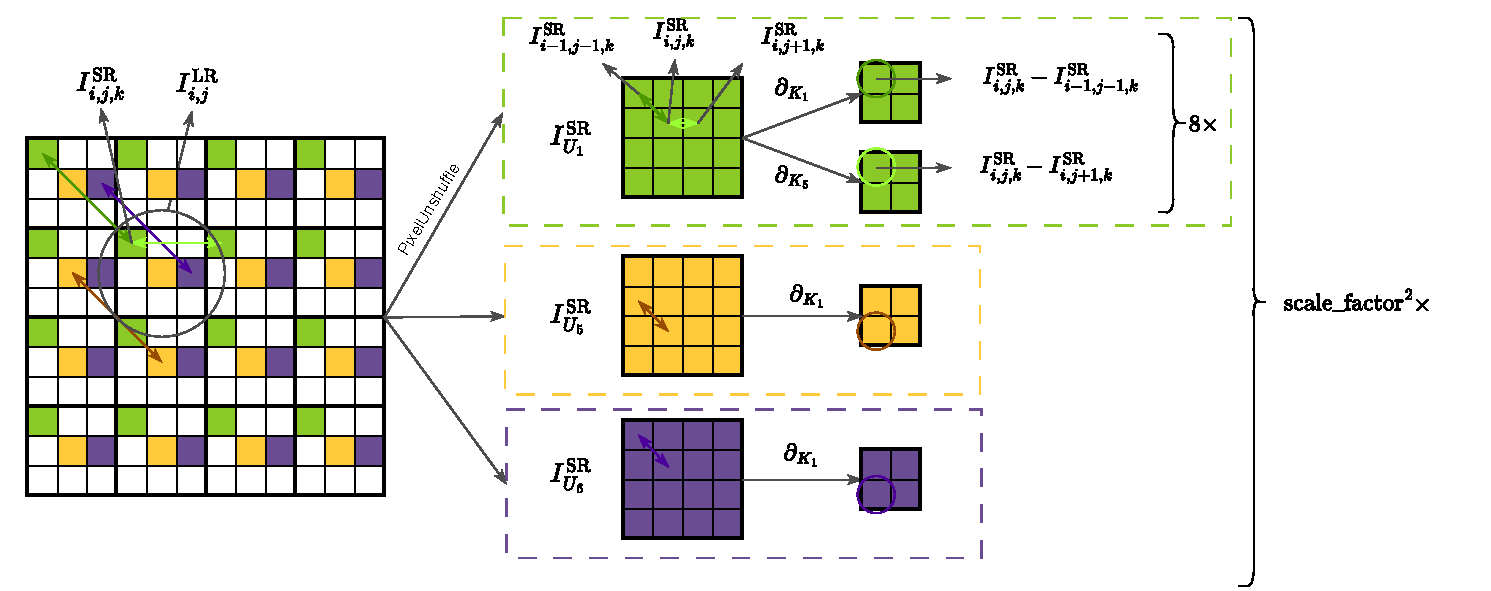
\includegraphics[width=\linewidth]{images/gloss.pdf}
        \caption[G-Loss patch derivatives]{
        G-Loss patch derivatives. 
        Downscaling factor $s = 3$ was used as example. 
        The indexation of the image is different than from the rest of the work.
        Here, the $I^\text{LR}_{i,j}$ corresponds to the pixel in the LR image in the $i$-th row and $j$-th column.
        This pixel is then downscaled producing pixels $\left\{I_{i,j,k}^\text{SR} \mid k \in \{1, 2, \dots s^2\}\right\}$.
        The derivative kernels are each of size $3\times3$ and are shown in Equation~\eqref{e:direction_kernels}. 
        No padding is added in convolution with derivative kernels.
        It is evident, that convolving the derivative kernels on the unshuffled patches is equivalent to convolving them with dilation.
        Furthermore, computing the mean over the unshuffled derivative patches (on the right side of the visualization) in direction $K_d$ produces the dilated derivative (Section~\ref{ss:dilated_sr_derivative}) in the direction $K_d$.
        For example, in the direction $K_1$ there are $s^2$ derivative patches (3 of them are shown on the right side).
        The element-wise mean of all the $s^2$ patches is equal to the dilated derivative in the direction $K_1$.
        }
        \label{fig:mean_sr_gradient}
    \end{figure}
\end{landscape}

\subsection{Hard constraints}

Hard constraints force the model to yield outputs that are consistent with the defined constraints.
In contrast to soft constraints (Section~\ref{ss:soft}), minimizing the constraint violation is insufficient in this case; the goal is to completely eliminate any constraint violation:
\begin{equation}
    \mathcal{L}_c = l\left(g\left(I^{\text{LR}}\right), h\left(I^{\text{SR}}\right)\right) = 0.
    \label{e:hard}
\end{equation}

To achieve the Equation~\eqref{e:hard}, model architecture changes are needed to guaranty the output's compliance with restrictions.
This change is implemented by adding one or more constraint layers.
Not every constraint in the form of Equation~\eqref{e:constraint} can be implemented straightforwardly as a hard constraint.

In a similar vein as soft constraint, Harder et al.~\cite{Harder2023} proposed the enforcement of the conservation law in the form of a hard constraint.
For the purpose of atmospheric gas concentration downscaling, Geiss et al.~\cite{Geiss2022} used a final constraining layer after SRCNN. 
However, this was not enough to improve the accuracy of the baseline model, except for ozone downscaling. 

\subsubsection{Non-negativity enforcing hard constraint layer}

Many variables cannot be negative, e.g., age, length, or climate related temperature in Kelvins.
Hence, it makes sense to have a non-negativity enforcing layer in some models.
To match the constraining setup (Section~\ref{ss:constraining}) we set 
\begin{equation}
\begin{aligned}
    \left(\forall I^{\text{LR}} \right) g\left(I^{\text{LR}}\right) = 0
    \ &\wedge \ 
h\left(I^{\text{SR}}\right) = \min_{i,j}\left(0, I^\text{SR}_{i,j}\right),
\end{aligned}
\end{equation}
therefore, the 
\begin{equation}
\mathcal{L}_s = g\left(I^{\text{LR}}\right) - h\left(I^{\text{SR}}\right)    
\end{equation}
will be zero if and only if all pixels in $I^\text{SR}$ are non-negative.
This trivial case could be solved by adding ReLU as the output layer of our network.

\subsubsection{General hard constraint layers}

For arbitrary constraints in the form as in our constraint setup (Section~\ref{ss:constraining}), there is no known general procedure to implement hard constraints.
We will need a more specific setup to automatically implement hard constraints.
\newpage
Harder et al. \cite{Harder2023} provided a generalization for constraining in the case of downscaling.
Suppose that we have an input LR image $I^{\text{LR}} \in \mathbb{R}^n$ and an output SR image $I^{\text{SR}} \in \mathbb{R}^m$.
Now $(S_j)_{j = 1, \dots, n}$ is a partition of $\{1, \dots, m\}$ into $n$ subsets, $g_{ij} : \mathcal{D} \subset \mathbb{R} \to \mathbb{R}, i \in S_j$ is an invertible function, and $h_j:\mathbb{R}^n \to \mathbb{R}$ is an arbitrary function.
The set of constraints is given by:
\begin{equation}
    \sum_{i\in S_j}g_{ij}\left(I^\text{SR}_i\right) = h_j\left(I^{\text{LR}}\right),
    \label{e:harder_constraint}
\end{equation}
for each $j = 1, \dots, n$.
Note that in downscaling with a scale factor of $s$, all the $S_j$ have a size of $s^2$.
Not every soft constraint mentioned in this work can be converted into a hard constraint.
Mainly, the approaches using the dilated derivatives cannot be expressed in the form of Equation~\eqref{e:harder_constraint} because the dilated derivative does not operate solely on the $s\times s$ patches, but also uses information from the neighboring patches.

Suppose that we have our general constraint in the form of Equation~\eqref{e:harder_constraint}.
Harder et al.~\cite{Harder2023} implemented three different approaches to a hard constraint layer -- additive, multiplicative, and soft-max layers.
These are defined by their output:
\begin{equation}
\begin{aligned}
    y_i^\text{AddCL} &= g_{ij}^{-1}\left( \tilde{y}_i + \frac{1}{s^2} h_j\left(I^{\text{LR}}\right) - \frac{1}{s^2} \sum_{k\in S_j}\tilde{y}_k \right), \\
    y_i^\text{MultCL} &= g_{ij}^{-1}\left( \tilde{y}_i \cdot \frac{h_j\left(I^{\text{LR}}\right)}{\sum_{k\in S_j}\tilde{y}_k }\right), \\
    y_i^\text{SmCL} &= g_{ij}^{-1}\left( \exp\left(\tilde{y}_i\right) \cdot \frac{h_j\left(I^{\text{LR}}\right)}{\sum_{k\in S_j}\exp\left(\tilde{y}_i\right) }\right), \\
\end{aligned}
\label{e:hard_constraint_layers}
\end{equation}
for $j = 1, \dots, n$, where the output from the unconstrained model is labeled as $\tilde{y}$.

\subsubsection{Conservation law}

Analogously to its soft-constraint counterpart (Section~\ref{sss:soft_conservation}), the enforced relation is that each LR pixel value is conserved and corresponds to the mean of the pixels generated from that specific pixel.
Formally, the enforced relation is:
\begin{equation}
    I^\text{LR}_{j} = \frac{1}{s^2} \sum_{i \in S_j}I^\text{SR}_{i}.
\end{equation}

The conservation law can be implemented as a hard constraint because it complies with Equation~\eqref{e:harder_constraint}.
This can be implemented with a standard deep learning model, augmented by an additional output layer -- a \textit{constraining layer} -- that modifies the model output in such a manner that the output LR pixel is equal to the mean of its corresponding downscaled SR pixels.
For this purpose, we will use the general Equations~\eqref{e:hard_constraint_layers} of hard constraint layers, with $g_{ij}$ being an identity function and $h_j(I^\text{LR}) = s^2 I^\text{LR}_j$.
The process of the additive constraint layer is depicted in Figure~\ref{fig:hard_conservation}.

\begin{figure}[htbp]
    \centering
    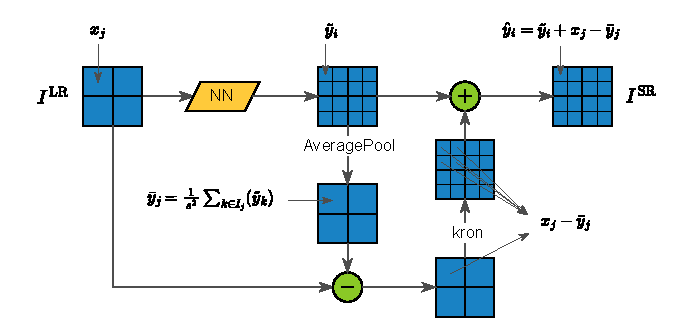
\includegraphics[width=\linewidth]{images/hard_conservation.pdf}
    \caption[Conservation law -- hard constraint]{Conservation law -- hard constraint. The operation ``kron'' denotes the Kronecker product (as defined in Section~\ref{sss:kronecker}) of the displayed matrix with an $s \times s$ matrix whose entries are all ones. Generating an output that matches the dimensions of the NN’s output.}
    \label{fig:hard_conservation}
\end{figure}

We will now prove that the implementation of the additive constraint layer (Equation~\eqref{e:hard_constraint_layers}) with the setup specified above and the implementation in Figure~\ref{fig:hard_conservation} is correct.

\begin{proof}
First, we state the output of the additive constraint layer (Equation~\eqref{e:hard_constraint_layers}) with the setup of $g_{ij}$ being an identity function and $h_j(I^\text{LR}) = s^2 I^\text{LR}_j$.
$$
I_i^\text{SR} = y_i^\text{AddCL} = \tilde{y}_i + I^\text{LR}_j - \frac{1}{s^2} \sum_{k\in S_j}\tilde{y}_k
$$
Now we calculate the means over areas $S_j$ for each $j$:
$$
\begin{aligned}
    \frac{1}{s^2} \sum_{i \in S_j} y_i^\text{AddCL} &=
    \frac{1}{s^2} \sum_{i \in S_j} \left(\tilde{y}_i + I^\text{LR}_j - \frac{1}{s^2} \sum_{k\in S_j}\tilde{y}_k \right) \\
    &= \frac{1}{s^2} \sum_{i \in S_j} \left(\tilde{y}_i \right) + I^\text{LR}_j - \frac{1}{s^2} \sum_{k\in S_j} \left(\tilde{y}_k \right) \\
    &= I_j^\text{LR}
\end{aligned}
$$
Thus, the means over areas of $S_j$ for each $j$ are equal to the corresponding input pixel $I_j^\text{LR}$.
\end{proof}

The proofs for the multiplicative and soft-max constraint layers closely follow the one given above; since the key step is merely replacing the output value, we do not present them here.

\subsubsection{Kronecker product}
\label{sss:kronecker}

The Kronecker product is a binary operation on two matrices of arbitrary sizes $A \in \mathbb{R}^{m_1, n_1}, B \in \mathbb{R}^{m_2, n_2}$, defined as:
\begin{equation}
    A \otimes B \coloneqq 
    \begin{bmatrix}
        A_{1,1} \cdot B & \cdots & A_{1, n} \cdot B \\
        \vdots & \ddots & \vdots \\ 
        A_{m, 1} \cdot B & \cdots & A_{m, n} \cdot B \\
    \end{bmatrix}.
\end{equation}
The result $A \otimes B$ is therefore the matrix $B$ multiplied by all scalars of $A$. 
For each of $m_1$ rows of $A$, the scalars will multiply $m_2$ rows of B; the same applies for columns, leading us to the dimension of the result being $(m_1 \cdot m_2) \times (n_1 \cdot n_2)$.

\subsection{Physical constraints}

There is not a distinct border between non-physical and physical constraints.
We consider any constraint that enforces physical laws, or that operates on physics-related quantities such as shape, gradients, and similar indicators, to be a physical constraint.

\section{Multivariate downscaling}

Multivariate downscaling refers to the simultaneous downscaling of several physical variables.
Furthermore, it allows for the incorporation of more complex physical relationships between the downscaled variables.
For example, Rocha et al.~\cite{Rocha2025} used up to five variables to downscale sea ice concentration.
Furthermore, Harder et al.~\cite{Harder2023} required surface temperature, liquid water, and water vapor in order to compute moist static energy, downscale the last three quantities and subsequently derive SR temperature from them.
However in this work we will focus solely on the mean temperature.

\section{Resampling}

There are several approaches for converting between HR and LR grids.
The simplest one is \textit{nearest} resampling, in which the value of a pixel at a new location is simply taken from the closest existing pixel.
A more advanced option is \textit{bilinear} interpolation, in which the value of the new pixel is obtained as a distance-weighted average of the surrounding pixels in the $2 \times 2$ neighborhood.
Both \textit{cubic} and \textit{cubic spline} methods use cubic polynomial approximations over $4 \times 4$ neighborhoods; however, cubic spline typically yields smoother transitions.
For more information about the above methods see Roszkowiak et al.~\cite{Roszkowiak2017}.
\textit{Lanczos} resampling relies on an even larger $6 \times 6$ neighborhood and evaluates the new pixel value using the $\text{sinc}$ function.
Detailed description can be found in Mazzoli~\cite{Mazzoli2026}.
When the value of a new pixel is obtained as the average over a neighborhood of arbitrary size, the procedure is referred to as \textit{average} resampling.


%---------------------------------------------------------------
\chapter{Experiments}
%---------------------------------------------------------------
\label{ch:experiments}

\section{Data}
\subsection{ReKIS}

\textit{Regionales Klimainformationssystem Sachsen, Sachsen-Anhalt, Thüringen} -- ReKIS -- is a regional climate information system operating in Central Germany. 
We will use its product \textit{KlimRefDS\_v3.1\_1961-2023}, which monitors several climate variables from 1961 to 2023.
This dataset will be used for training purposes in LR and HR pairs, where the LR images will be resampled from this HR dataset.

\begin{figure}[htbp]
    \centering
    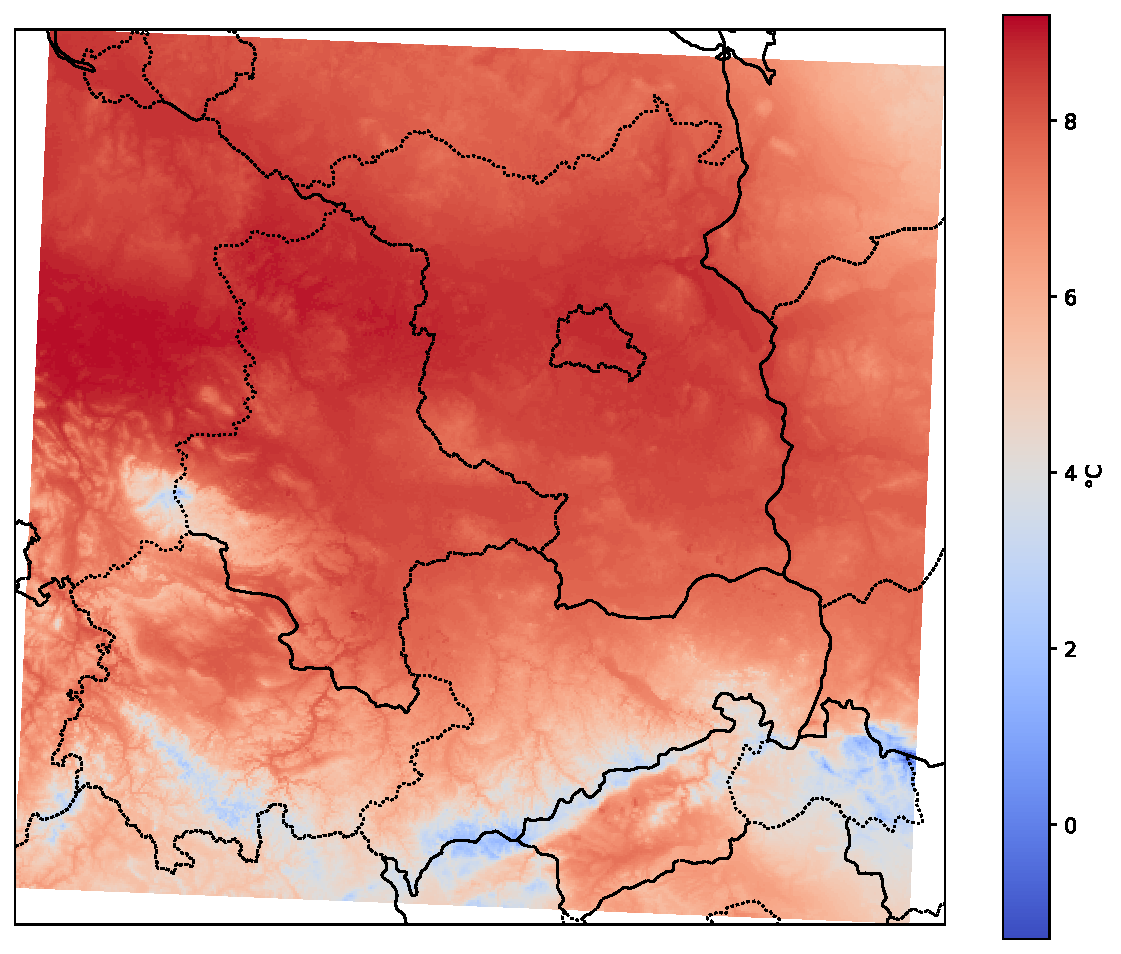
\includegraphics[width=0.7\linewidth]{images/rekis.pdf}
    \caption[ReKIS example]{ReKIS example. The mean temperature on 2000-02-01 is shown.}
    \label{fig:rekis_2000_02_01}
\end{figure}

\begin{description}
    \item[Region.] The studied region is Central Germany, mainly the area of the constituent states of Saxony, Saxony-Anhalt, and Thuringia. 
    This region does not form a square on the map; therefore, data from other neighboring German constituent states, Poland, and Czechia were included. 
    \item[Variables.] The data collected consist of multiple climate variables, which are listed in Table~\ref{tab:ReKISdata}.
    These variables are present in daily, monthly, and annual means.
    In this work, we will focus on daily mean temperature.
    \item[Grid.] Data were obtained from observational meteorological stations.
    From these stations, ReKIS produced grids for each variable using interpolation, in the form displayed in Figure~\ref{fig:rekis_2000_02_01}.
\end{description}

{
\shorthandoff{-}
\begin{table}[htbp]
    \centering
    \begin{tabular}{|l|c|l|}
        \hline
        \textbf{Variable name}              & \textbf{Unit} & \textbf{Note} \\ 
        \hline
        Vapor pressure                     & $\text{hPa}$ & Daily mean \\ 
        \hline
        Saturation vapor pressure          & $\text{hPa}$ & Daily mean \\ 
        \hline
        \multirow{2}{*}{Potential evaporation}              & $\text{mm} \cdot \text{day}^{-1}$ & Daily sum \\ 
        \cline{2-3}
        & $\text{W} \cdot \text{m}^{-2}$ & Daily mean \\         
        \hline
        Mean wind speed                    & $\text{m} \cdot \text{s}^{-1}$ & Daily mean \\ 
        \hline
        Maximum wind speed                 & $\text{m} \cdot \text{s}^{-1}$ & Daily maximum \\ 
        \hline
        \multirow{2}{*}{Grass reference evapotranspiration} & $\text{mm} \cdot \text{day}^{-1}$ & Daily sum \\ 
        \cline{2-3}
        & $\text{W} \cdot \text{m}^{-2}$ & Daily mean \\ 
        \hline
        Relative humidity                  & $\text{\%}$ & Daily mean \\ 
        \hline
        \multirow{2}{*}{Global solar radiation} & $\text{J} \cdot \text{cm}^{-2}$ & Daily sum \\ 
        \cline{2-3}
        & $\text{W} \cdot \text{m}^{-2}$ & Daily mean \\ 
        \hline
        Corrected precipitation            & $\text{mm} \cdot \text{day}^{-1}$ & Daily sum \\ 
        \hline
        Uncorrected precipitation          & $\text{mm} \cdot \text{day}^{-1}$ & Daily sum \\ 
        \hline
        Mean temperature                   & $^\circ\text{C}$ & Daily mean \\ 
        \hline
        Minimum temperature                & $^\circ\text{C}$ & Daily minimum \\ 
        \hline
        Maximum temperature                & $^\circ\text{C}$ & Daily maximum \\ 
        \hline
    \end{tabular}
    \caption[ReKIS climate variables]{ReKIS climate variables.}
    \label{tab:ReKISdata}
\end{table}
}

The area covered by ReKIS is predominantly flat in its northern and central parts, while its southern section is characterized by mountainous terrain.
The high elevation also influences the mean temperature, which is visible both in the one day mean Figure~\ref{fig:rekis_2000_02_01} and in Figure~\ref{fig:rekis_mean}, which depicts the mean temperature from 1961 to 1992.
It is clear that the HR structures and distinct boundaries, particularly the warm temperature corridors in mountainous areas, are also retained in the mean temperature field.
These are characteristics that cannot be completely captured in LR images, and the models will need to handle them accordingly.

\begin{figure}[htbp]
    \centering
    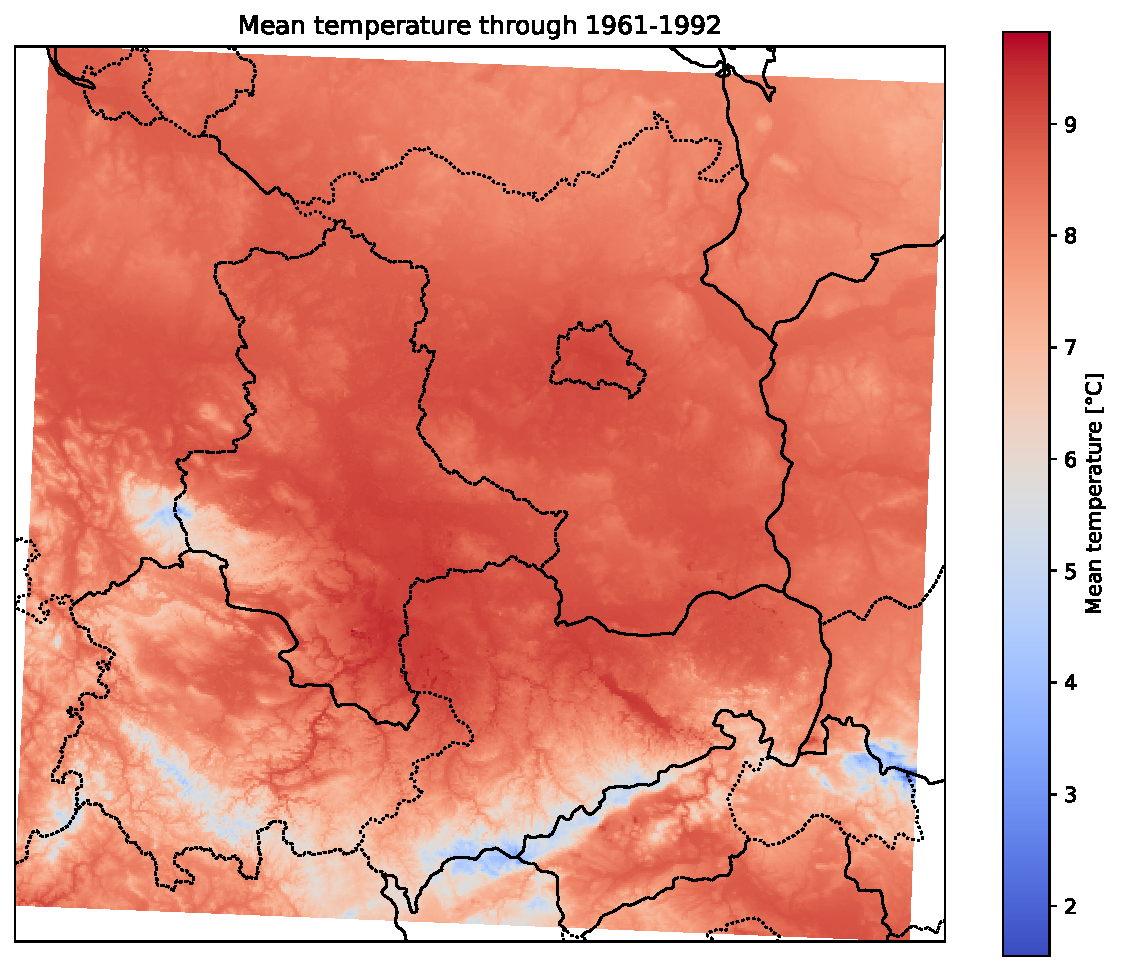
\includegraphics[width=0.7\linewidth]{images/rekis_mean.pdf}
    \caption[ReKIS mean temperature through 1961--1992]{ReKIS mean temperature through 1961--1992.}
    \label{fig:rekis_mean}
\end{figure}

\subsection{EURO-CORDEX}

The European Coordinated Downscaling Experiment -- EURO-CORDEX -- as its name suggests, is an ensemble of regional climate downscaling experiments~\cite{Jacob2014}.
One of them is REMO2015, an experiment where the regional climate model REMO was run on the boundary conditions of the global climate model ERA-Interim reanalysis.
We will use this experiment, more specifically its evaluation version (where the model was run on past conditions), with a resolution of $0.11^\circ$ (12.5 km) from the years 1979 to 2012.
This experiment covers the whole of Europe and provides several climate variables; however, we will use only daily mean temperature.
For the sake of simplicity, we will refer to this dataset as the EURO-CORDEX dataset in this work, even though it is only a small fraction of the EURO-CORDEX example and even from the REMO2015 experiment.
An example is shown in Figure~\ref{fig:cordex}.

\begin{figure}
    \centering
    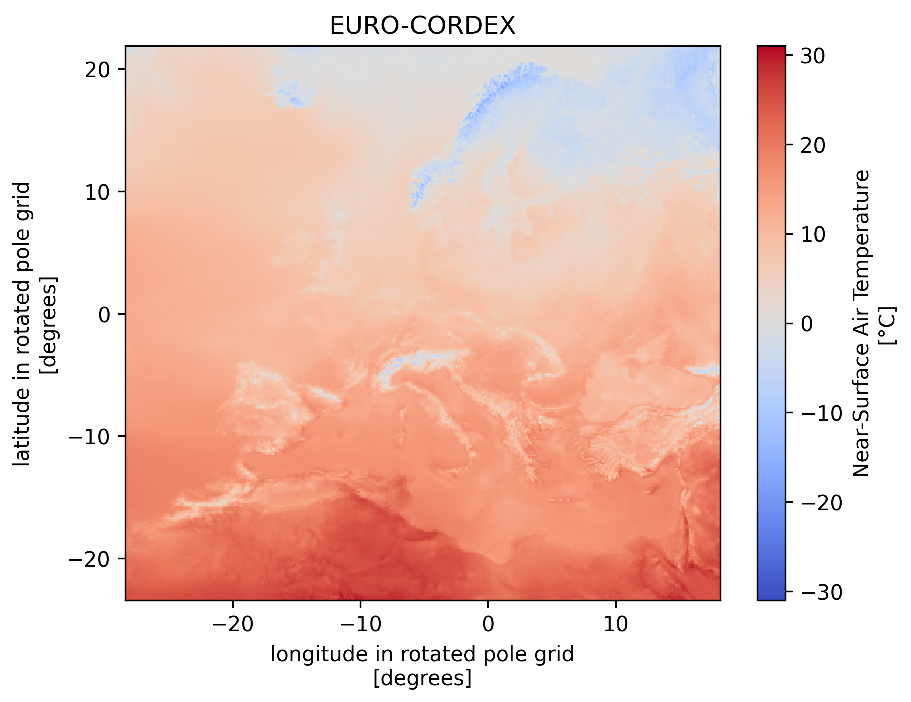
\includegraphics[width=0.8\linewidth]{images/cordex.pdf}
    \caption[EURO-CORDEX example]{EURO-CORDEX example. The mean temperature on 2000-02-01 is shown.}
    \label{fig:cordex}
\end{figure}

\subsection{Workflow}

Our primary goal is to downscale the climate projections (EURO-CORDEX).
However, those do not have a HR version.
Therefore, we incorporate the observational gridded dataset (ReKIS), where the HR data are available.
Then we produce LR images from them using a resampling method and train the model on these observational LR and HR pairs.
We also evaluate the models on the observational data and choose the best one, which will be applied to LR projections, yielding the final HR predictions.
This process is visualized in Figure~\ref{fig:workflow}.

\begin{figure}
    \centering
    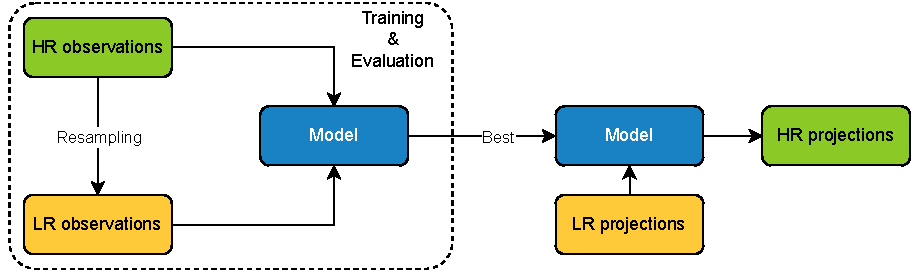
\includegraphics[width=\linewidth]{images/workflow.pdf}
    \caption[Workflow]{Workflow. Initially the model is trained on the observations, which are available in HR version, and can be resampled to LR version. We evaluate and choose the best model on the observations. Then we apply the best model to LR predictions. The LR data are highlighted in yellow, the HR in green and the models in blue.}
    \label{fig:workflow}
\end{figure}

\subsection{Data preprocessing}

For the work with geospatial data, we used the rioxarray package.
ReKIS and the EURO-CORDEX data have different coordinate reference systems (CRS).
ReKIS uses the 3-degree Gauss-Kruger zone 4, whereas EURO-CORDEX uses the World Geodetic System 1984.
We will reproject the EURO-CORDEX data to match ReKIS's CRS.

The grid from ReKIS was cropped to $400 \times 400$ HR images.
These images are then downsampled to a lower resolution to generate the LR images, which are divided into three groups by year: a training set (1961--1992), a validation set (1993--2002), and a test set (2003--2012).
The division by years is to simulate the predictions of the model on unseen data, which can have a different distribution than the observed ones.
We restrict ourselves to ReKIS data up to 2012, even though data are available through 2023, because we also need to retain unseen data within the EURO-CORDEX dataset.


\section{Resampling method}
\label{s:resampling_method_exp}

Before any training can take place, it is necessary to have LR and HR pairs prepared.
The HR parts are from ReKIS, and the LR parts need to be obtained by resampling the HR images.
However, there are more methods for such transformation -- nearest, bilinear, cubic, cubic spline, Lanczos, and average resampling.
The differences are visible in the example of the mean temperature on 2000-02-01 in Figure~\ref{fig:resampling}.
The smoothest LR image appears to be the one generated by cubic spline, whereas the one with the highest changes between its neighbors is generated by the nearest resampling.
The concept of dilated derivative consistency applies exclusively to resampling methods that can be expressed as a convolution with a fixed kernel; among the methods mentioned, only average resampling fulfills this requirement.
Košťál et al.~\cite{Kostal2025} applied cubic spline, whereas Harder et al.~\cite{Harder2023} referred to average resampling as the ``standard methodology in climate downscaling studies''.
The upcoming Sections (\ref{ss:performance_resampling} and \ref{ss:violation_resampling}) will examine which is the most advantageous for our specific use case.

\begin{figure}[htbp]
    \centering
    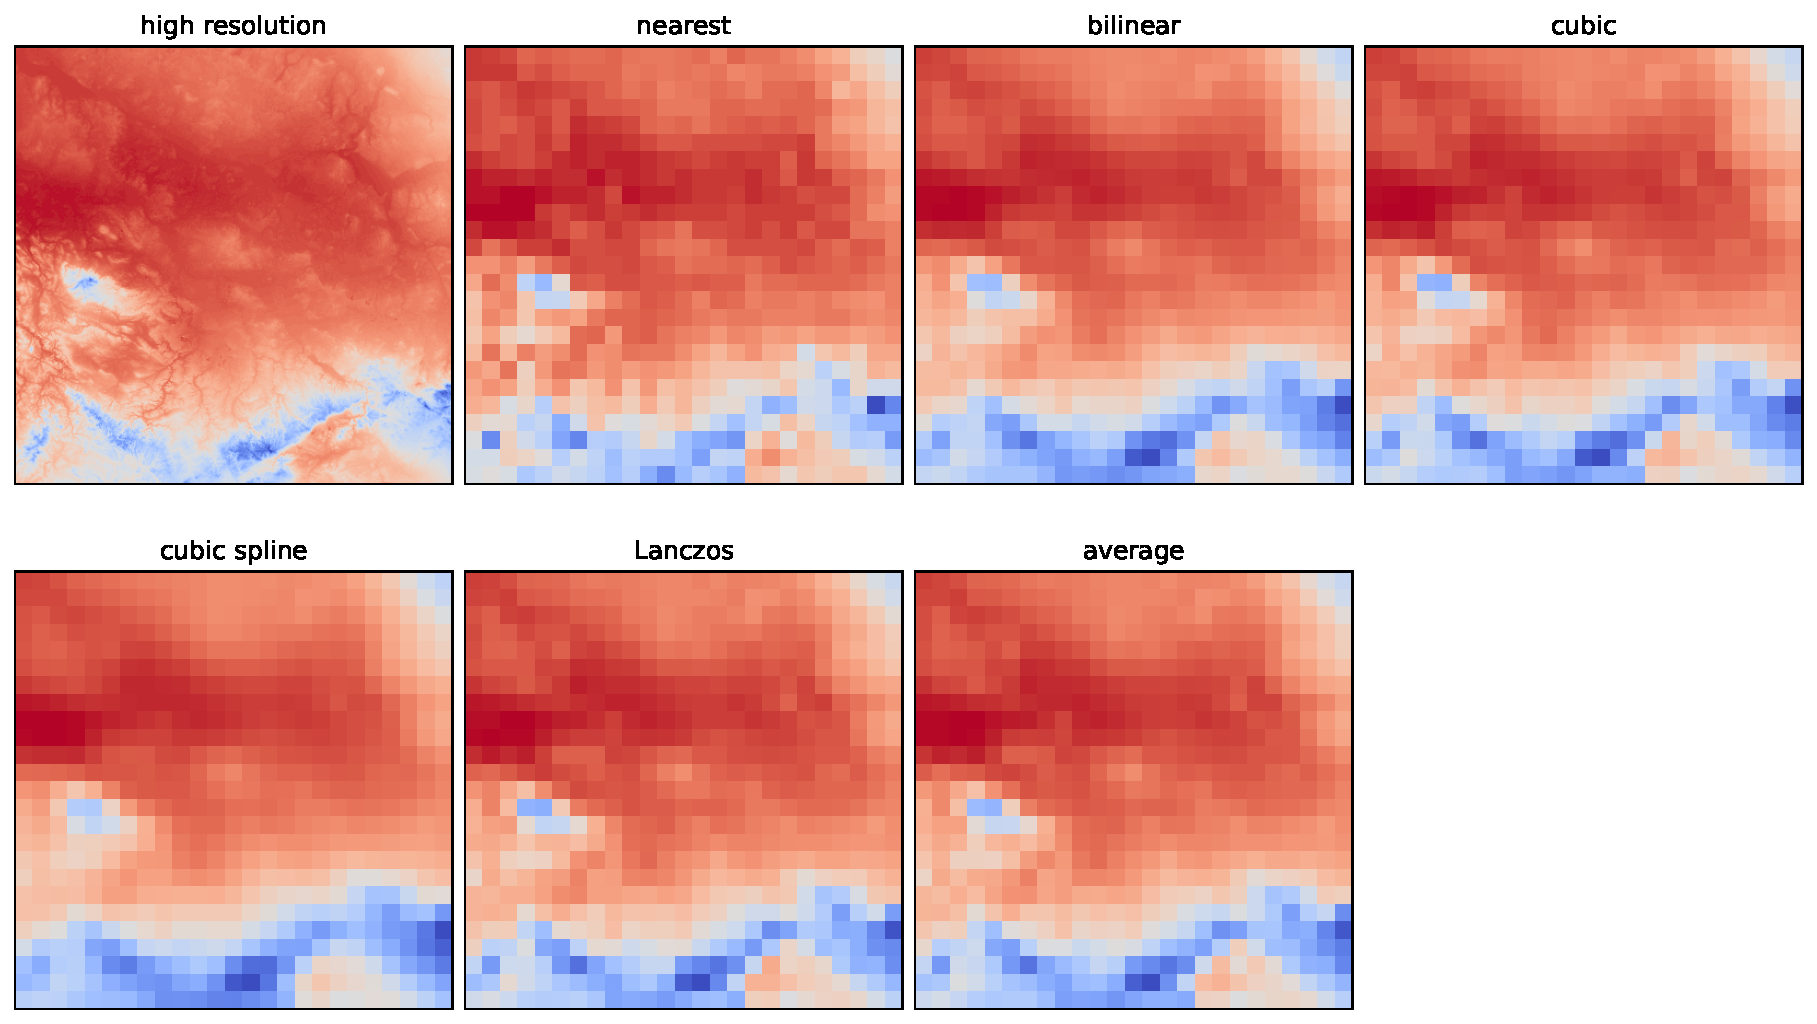
\includegraphics[width=\linewidth]{images/resampling.pdf}
    \caption[Resampling methods]{Resampling methods. The original HR image is shown on the left top of the figure, then six examples of resampling -- nearest, bilinear, cubic, cubic spline, Lanczos, and average -- have been applied on it. The results of resampling the HR image with scale factor of 16 are shown. The HR image from ReKIS shows mean temperature on 2000-02-01.}
    \label{fig:resampling}
\end{figure}

\subsection{Model performance orientated choice of resampling method}
\label{ss:performance_resampling}

One approach to decide which resampling method will be used is to measure the model performance on both resampling methods.
For better comparison, we include more scale factors and an unconstrained model, a soft-constrained model, and a hard-constrained model.
For the model, we choose EDSR with 128 residual blocks and 64 features, exactly as in the best model by Košťál et al.~\cite{Kostal2025}.
As representatives of both soft and hard constraints, we use the conservation law, since it is the only constraint in this work that can be implemented both ways. 
Therefore, the focus will be on the implementation, not on the appropriateness of the physical principle.
As the conservation soft constraint version, we choose squared, and the $\alpha$ parameter equal to $10^{-4}$, both the same as Harder et al.~\cite{Harder2023}.
Hard constraining is implemented as an additive constraint layer because it performs the best among the three possibilities (Section~\ref{s:hard_constraint_exp}). 
We include both cubic spline and average pooling, used by Košťál et al.~\cite{Kostal2025} and Harder et al.~\cite{Harder2023}.

All the results are shown in Figure~\ref{fig:scale_factor_model_type}.
Much new information can be observed there.
First, when using hard constraints with the cubic spline, the performance was significantly worse than both the average resampling scenario and the other types of constraints applied in the cubic spline setting.
This can be caused by the fact that the hard constraining layer is enforcing a relation -- conserving the mean through downscaling -- that is not present even between LR and target HR images, as will be shown in Section~\ref{ss:violation_resampling}.
Next, the hard constraint using the average resampling method was applied across all scale factors within the best configurations, also shown in Table~\ref{tab:best_for_scale_factor}. 
Moreover, the final configuration demonstrated a stabilizing effect on model performance as the scale factor increased, whereas the other configurations exhibited greater volatility.
Starting from a scale factor of 40, the model’s RMSE values began to rise sharply.
Yet, even at this scale, the input LR image is only $10 \times 10$, while the model generates SR images of size $400 \times 400$.
In other words, the model must infer $1600$ SR pixels from a single LR pixel, which is understandably challenging and contributes to the increased error produced by the model.

\begin{figure}[htbp]
    \centering
    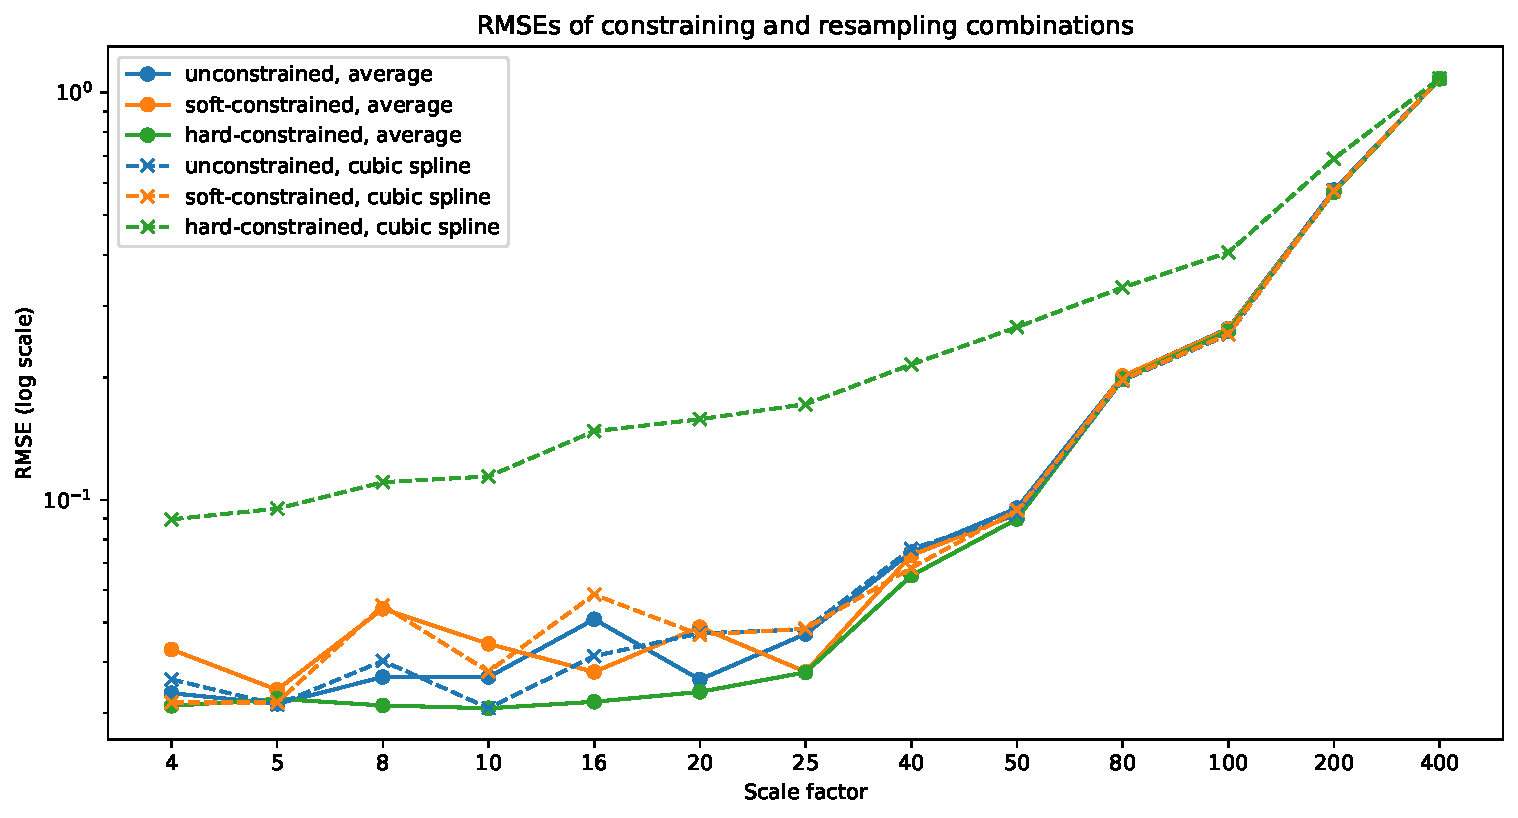
\includegraphics[width=\linewidth]{images/resampling_plot.pdf}
    \caption[Scale factor and model types performances]{Scale factor and model types performances.}
    \label{fig:scale_factor_model_type}
\end{figure}

\begin{table}[htbp]
    \centering
    \begin{tabular}{|c|l|c|c|}
        \hline
         \textbf{scale factor} &  \textbf{RMSE} & \textbf{resampling method} & \textbf{constraining} \\
         \hline \hline
         $4\times$ & 0.0312 & average & hard \\ \hline 
         $5\times$ & 0.03142 & cubic spline & unconstrained \\ \hline 
         $8\times$ & 0.03128 & average & hard \\ \hline 
         $10\times$ & 0.03078 & average & hard \\ \hline 
         $16\times$ & 0.03193 & average & hard \\ \hline 
         $20\times$ & 0.03377 & average & hard \\ \hline 
         $25\times$ & 0.03772 & average & hard \\ \hline 
         $40\times$ & 0.06515 & average & hard \\ \hline 
         $50\times$ & 0.08976 & average & hard \\ \hline 
         $80\times$ & 0.19673 & cubic spline & unconstrained \\ \hline 
         $100\times$ & 0.25454 & cubic spline & unconstrained \\ \hline 
         $200\times$ & 0.57030 & average & hard \\ \hline 
         $400\times$ & 1.08279 & average & hard \\ \hline 
    \end{tabular}
    \caption[Best models for each scale factor]{Best model type and resampling method pairs are shown for each scale factor.}
    \label{tab:best_for_scale_factor}
\end{table}

Focusing on the improvement of the constrained models with respect to the unconstrained one, it is evident that using average resampling, the majority of runs yielded better results when the hard constraint was present (Figure~\ref{fig:res_rel_avg}).
Exactly the opposite can be observed in the cubic spline case, where the hard constrained models have shown worse performance than the unconstrained versions (Figure~\ref{fig:res_rel_cs}).
In both settings, soft constraining shows balancing ratios on the edge of improvement.
The most significant improvement was achieved for the hard constrained model with average resampling downscaling with a scale factor of 16.

\begin{figure}[htbp]
    \centering
    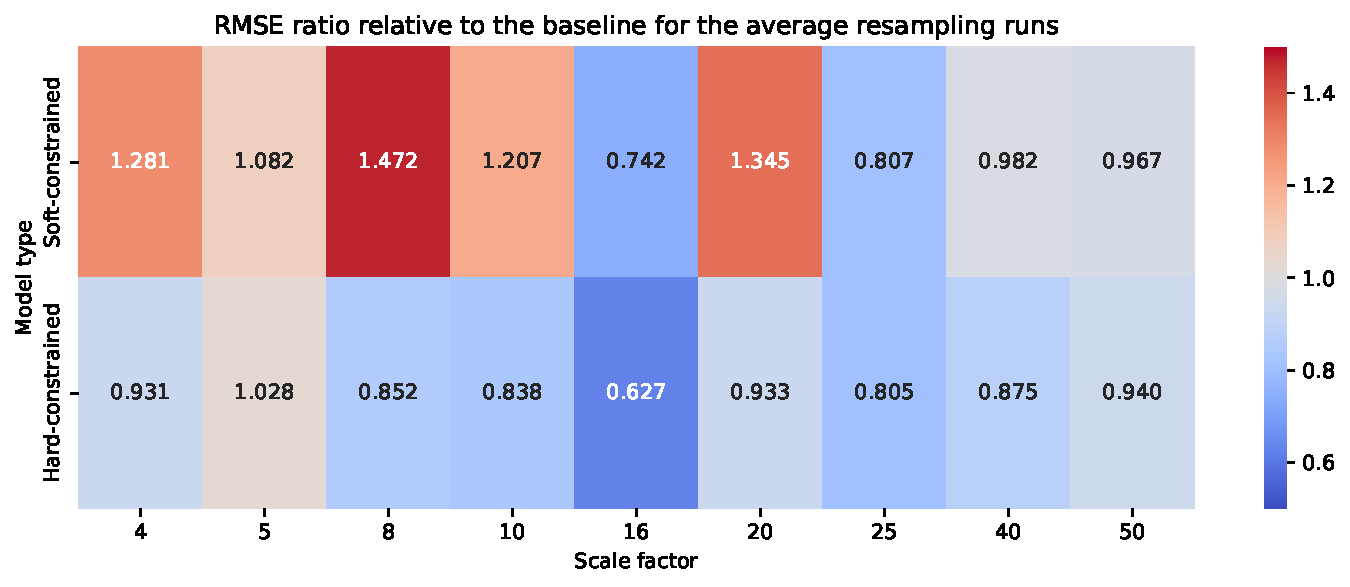
\includegraphics[width=0.75\linewidth]{images/resampling_rel_avg_9.pdf}
    \caption[Relative model improvement across scale factors in the average resampling setting]{Relative model improvement across scale factors in the average resampling setting.}
    \label{fig:res_rel_avg}
\end{figure}

\begin{figure}[htbp]
    \centering
    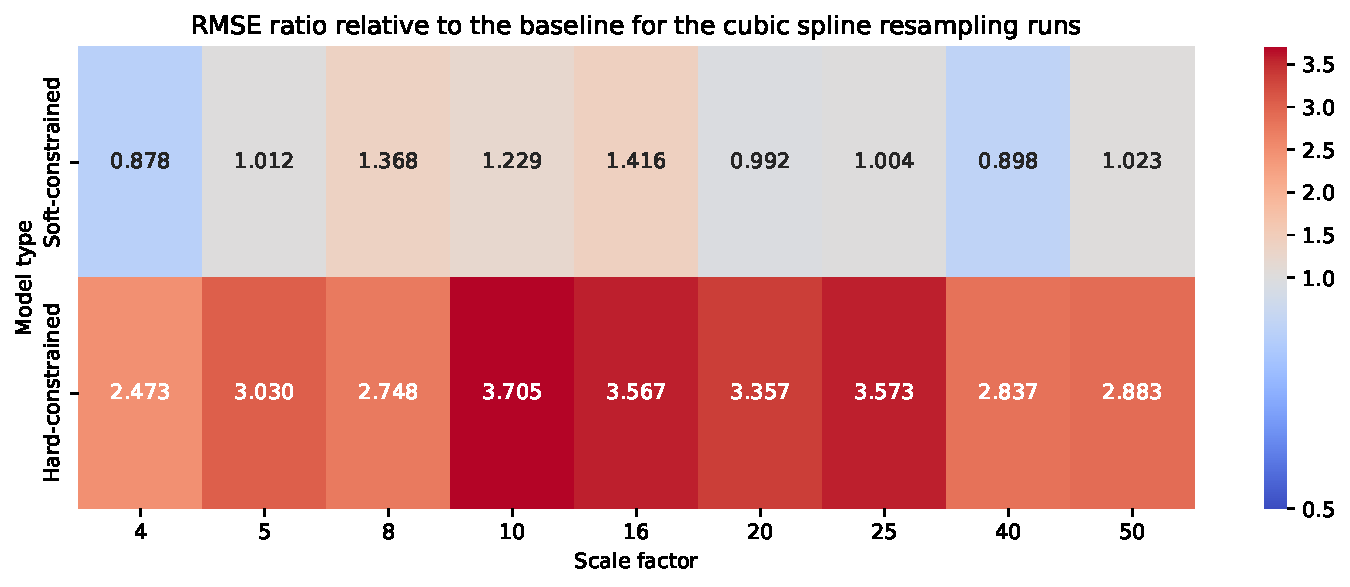
\includegraphics[width=0.75\linewidth]{images/resampling_rel_cs_9.pdf}
    \caption[Relative model improvement across scale factors in the cubic spline resampling setting]{Relative model improvement across scale factors in the cubic spline resampling setting. Note that the color palette is non-linear; it has been adjusted so that the blue values indicate improvement relative to the corresponding baseline model.}
    \label{fig:res_rel_cs}
\end{figure}

\subsection{Target violation orientated choice of resampling method}
\label{ss:violation_resampling}

The fundamental property of a constraint should be that the violation is equal to zero for LR and HR pairs.
That is the best a hypothetical model could achieve when trained under a particular constraint. 
Therefore, we will calculate the mean violation for each constraint on the train ReKIS dataset.
The results are visible in Table~\ref{tab:resampling_soft_exp}.
It is clearly visible that average pooling dominates other methods and confirms the role of ``standard methodology''~\cite{Harder2023}.
In the remainder of this work, average pooling will be implicitly adopted as the resampling method, as it achieved the best performance in both experiments.

\begin{landscape}
{
\shorthandoff{-}
\begin{table}[htbp]
    \centering
    \begin{tabular}{|l|c|l|l|l|l|l|l|}
        \hline
        \textbf{Constraint name} & \textbf{Version} & \textbf{nearest} & \textbf{bilinear} & \textbf{cubic} & \textbf{cubic spline} & \textbf{Lanczos} & \textbf{average} \\ 
        \hline
        \hline
        \multirow{2}{*}{Conservation law} & absolute & 0.13428 & 0.03583 & 0.0225 & 0.07657 & 0.03859 & \textbf{0.00001} \\ 
        \cline{2-8}
        & squared & 0.05433 & 0.00387 & 0.00137 & 0.01738 & 0.00402 & \textbf{0} \\
        \hline
        \multirow{2}{*}{Simple derivative} & absolute & 0.38241 & 0.1024 & 0.0609 & 0.2038 & 0.10007 & \textbf{0} \\ 
        \cline{2-8}
        & squared & 0.21994 & 0.01661 & 0.00563 & 0.06648 & 0.01475 & \textbf{0}  \\       
        \hline
        \multirow{2}{*}{Sobel gradient magnitude} & absolute & 0.48015 & 0.14631 & 0.08667 & 0.35088 & 0.17259 & \textbf{0} \\ 
        \cline{2-8}
        & squared & 0.63199 & 0.06462 & 0.01989 & 0.37543 & 0.08638 & \textbf{0}  \\       
        \hline
        \multirow{2}{*}{Continuity} & absolute & 0.16535 & 0.06096 & 0.00156 & 0.12777 & 0.0341 & \textbf{0} \\ 
        \cline{2-8}
        & squared & 0.3045 & 0.09947 & 0.00484 & 0.19380 & 0.06993 & \textbf{0} \\         
        \hline
        \multirow{2}{*}{G-Loss} & absolute & 0.19072 & 0.0511 & 0.03032 & 0.10464 & 0.05038 & \textbf{0} \\ 
        \cline{2-8}
        & squared & 0.10876 & 0.00825 & 0.00273 & 0.03446 & 0.00735 & \textbf{0} \\        
        \hline
        \multirow{2}{*}{Simple gradient direction} & absolute & 0.07963 & 0.00476 & 0.00285 & 0.01708 & 0.00636 & \textbf{0} \\ 
        \cline{2-8}
        & squared & 0.04772 & 0.00058 & 0.00015 & 0.00471 & 0.00062 & \textbf{0} \\        
        \hline
        \multirow{2}{*}{Sobel gradient direction} & absolute & 0.09696 & 0.00477 & 0.00222 & 0.02248 & 0.00683 & \textbf{0} \\ 
        \cline{2-8}
        & squared & 0.09551 & 0.00037 & 0.00008 & 0.00646 & 0.00068 & \textbf{0} \\        
        \hline
    \end{tabular}
    \caption[Resampling and soft constraints]{Resampling and soft constraints. For each constraint type, six resampling methods are evaluated by measuring the violation between the HR image and the resampled LR image. The best result for each soft constraint is shown in \textbf{bold}. From these experiments, average pooling clearly emerges as the most effective resampling technique among those tested.
    Note that this outcome is expected: when average resampling is used, derivative consistency holds (Section~\ref{ss:dilated_sr_derivative}), leading to identical derivatives. 
    As a result, the constraints cannot penalize any difference between them.
    The values were rounded to 5 decimal places.
    }
    \label{tab:resampling_soft_exp}
\end{table}
}
\end{landscape}

\section{Hard constraint type}
\label{s:hard_constraint_exp}

As shown in Equations~\eqref{e:hard_constraint_layers}, there are three types of hard constraint layers: additive, multiplicative, and soft-max layer.
We will conduct an experiment to determine which one will be used further on.

The results in Table~\ref{tab:hard_constraint_implementation} indicate that the multiplicative method performs significantly worse than the other two approaches. 
Moreover, the soft-max variant still exhibits an RMSE that is more than twice as large as that of the additive layer.
We consider this to be a huge difference, and in this work, we will always use the additive implementation.

\begin{table}[htbp]
    \centering
    \begin{tabular}{|l|l|l|}
        \hline
         \textbf{Type} & \textbf{MAE} & \textbf{RMSE} \\
         \hline \hline
         additive & \textbf{0.02603} & \textbf{0.0315} \\
         \hline
         multiplicative & 0.14764 & 0.25448 \\
        \hline
        soft-max & 0.03481 & 0.07369 \\
        \hline
    \end{tabular}
    \caption[Hard constraint layer implementation experiment]{Hard constraint layer implementation experiment.}
    \label{tab:hard_constraint_implementation}
\end{table}

Both the multiplicative and soft-max constraint layers encounter difficulties when the mean temperature is near 0$^\circ$C because of the division involved (Equations~\eqref{e:hard_constraint_layers}).
In addition, the soft-max layer preserves the sign of the LR pixel across all of its corresponding downscaled pixels.
Yet, 0$^\circ$C does not have a special thermodynamic significance like 0K, so preserving the sign in this way is not particularly beneficial.

\section{Soft constraint type}
\label{s:constraints_exp}

Initially, we analyze how each soft constraint affects the models' performance.
We follow Košťál et al.~\cite{Kostal2025} and, as the model type, we choose EDSR with 64 channels and 128 residual blocks.
We use the constraint loss ratio $\alpha = 10^{-4}$, the same as the best value used by Harder et al.~\cite{Harder2023}.
In each experiment, we choose a constraint and a type of penalty, and train the model above with this configuration. 
The scale factor applied in this experiment is the one for which the constraining yielded the greatest improvement (Section~\ref{ss:performance_resampling}) -- namely, $16\times$.

The results are shown in Table~\ref{tab:soft_constraints_exp}.
The best constraint was the one penalizing the difference in the derivatives calculated by the simple kernels.
The second best was the modified G-Loss constraint.
There is no consistent dominance of any version of the interested constraints.
All the runs have produced reasonable results.

{
\shorthandoff{-}
\begin{table}[htbp]
    \centering
    \begin{tabular}{|l|c|l|l|}
        \hline
        \textbf{Constraint name} & \textbf{Version} & \textbf{MAE} & \textbf{RMSE} \\ 
        \hline
        \hline
        \multirow{2}{*}{Conservation law} & absolute & 0.03776 & 0.05392 \\ 
        \cline{2-4}
        & squared & 0.0278 & 0.0378 \\         
        \hline
        \multirow{2}{*}{Simple derivative} & absolute & \textbf{0.02709} & \textbf{0.0358} \\ 
        \cline{2-4}
        & squared & 0.04662 & 0.06364 \\         
        \hline
        \multirow{2}{*}{Sobel gradient magnitude} & absolute & 0.0304 & 0.0432 \\ 
        \cline{2-4}
        & squared & 0.04159 & 0.0594 \\         
        \hline
        \multirow{2}{*}{Continuity} & absolute & 0.03032 & 0.04301 \\ 
        \cline{2-4}
        & squared & 0.04211 & 0.0583 \\         
        \hline
        \multirow{2}{*}{G-Loss} & absolute & \textit{0.02762} & \textit{0.03750} \\ 
        \cline{2-4}
        & squared & 0.03812 & 0.05429 \\         
        \hline
        \multirow{2}{*}{Simple gradient direction} & absolute & 0.0452 & 0.06299 \\ 
        \cline{2-4}
        & squared & 0.03959 & 0.05652 \\         
        \hline
        \multirow{2}{*}{Sobel gradient direction} & absolute & 0.05167 & 0.07144 \\ 
        \cline{2-4}
        & squared & 0.03071 & 0.04287 \\         
        \hline
    \end{tabular}
    \caption[Constraint types experiment]{Constraint types experiment. Best result is highlighted in \textbf{bold}, the second best in \textit{italics}.}
    \label{tab:soft_constraints_exp}
\end{table}
}

\section{Soft constraint alpha value}
\label{s:soft_constraints_alpha_exp}

We conduct a simple search for the optimal $\alpha$ for the best constraint type from Section~\ref{s:constraints_exp} -- the absolute version of the simple derivative constraint.
The $\alpha$ value, as described in Equation~\eqref{e:soft_constraint}, determines the relative influence of the constraint with respect to the pixel-wise loss.

Results are shown in Table~\ref{tab:alpha_exp}.
It is evident that placing excessive emphasis on minimizing the constraint violation (high $\alpha$) over pixel-wise loss is not improving the model's performance.
The best alpha value was $10^{-4}$, the same as in Harder et al.~\cite{Harder2023}; however, this is a different constraint with possibly a different range.
Moreover, it is clearly demonstrated that including a certain amount of physical information, with the weight $\alpha$ in the range of $10^{-5}$ to $10^{-2}$, has a beneficial impact compared to a model that relies only on a pixel-wise loss function ($\alpha = 0$).

\begin{table}[htbp]
    \centering
    \begin{tabular}{|l|l|l|}
        \hline
         $\mathbf{\alpha}$ & \textbf{MAE} & \textbf{RMSE} \\
         \hline
         \hline
         1 & 2.91212 & 4.2134 \\
         \hline
         0.99999 & 2.82308 & 4.08568 \\
         \hline
         0.9999 & 0.33783 & 0.65158 \\
         \hline
         0.999 & 0.18782 & 0.31223 \\
         \hline
         0.99 & 0.16098 & 0.27225 \\
         \hline
         0.9 & 0.03794 & 0.05481 \\
         \hline
         0.5 & 0.0291 & 0.04008 \\
         \hline
         0.1 & 0.03978 & 0.05556 \\
         \hline
         0.01 & 0.05832 & 0.08171 \\
         \hline
         0.001 & \textit{0.0281} & \textit{0.03862} \\
         \hline
         0.0001 & \textbf{0.02709} & \textbf{0.0358} \\
         \hline
         0.00001 & 0.02975 & 0.04134 \\
         \hline
         0 & 0.03569 & 0.05092 \\
         \hline
    \end{tabular}
    \caption[Soft constraining alpha experiments]{Soft constraining alpha experiments. Best results are highlighted in \textbf{bold}, the second best in \textit{italics}.}
    \label{tab:alpha_exp}
\end{table}

\section{Model size}
\label{s:models_size_exp}

We study how the model size -- the number of the model's trainable parameters -- affects its performance.
The question of size arises from the usage of the smaller SRCNN in Harder et al.~\cite{Harder2023} compared to the larger EDSR in Košťál et al.~\cite{Kostal2025}.
We inspect EDSR model types with $r \in\{ 1, 2, 4, 8, 16, 32, 64, 128 \}$ residual blocks and $f \in\{ 1, 2, 4, 8, 16, 32, 64, 128 \}$ features -- channels used in residual blocks -- for unconstrained, soft conservation constraint, and hard conservation constraint.
The conservation constraint is chosen because it is the only one in this work that has both soft and hard constraint implementations, allowing us to compare the two approaches.
All the models will perform downscaling with a scale factor of 16.

The EDSR model size is dependent on the previously stated number of residual blocks $r$ and the number of channels $f$ used in those.
First, in a convolutional layer with a kernel size of $k \times k$ and $c_{in}$ input channels, $c_{in}$ different kernels are used for the convolution with the $c_{in}$ input channels, after that an element-wise sum is calculated and a bias is added, producing one of $c_{out}$ output channels.
This corresponds to the overall number of parameters being:
\begin{equation}
    p_\text{CL} = \left(k^2 \cdot c_{in} + 1\right) \cdot c_{out}.
\end{equation}
Throughout all the EDSR convolutional layers, only a kernel size of $3 \times 3$ is used.
The head of the EDSR model consists of a single convolutional layer, the task of which is to produce $f$ channels from the single input channel. 
Thus, the number of parameters in the head is equal to:
\begin{equation}
    p_\text{head} = \left(3^2 \cdot 1 + 1\right) \cdot f = 10f.
\end{equation}
In the body, firstly $r$ residual blocks are present, each with two convolutional layers with $f$ input and $f$ output channels.
After them an additional convolutional layer is used with the same configuration.
The number of learnable parameters in the body is:
\begin{equation}
    p_\text{body} = \left(3^2 \cdot f + 1\right) \cdot f \cdot (2r + 1) = 18f^2r + 9f^2 + 2fr + f.
\end{equation}
In the tail, the upsampling takes place.
For each prime factor $p_i$ of scale factor $s$ a convolutional layer with $f$ input channels and $f\cdot p_i^2$ output channels is employed, followed by a pixel shuffle layer, which does not have any learnable parameters and only reshapes its input to have $f$ channels again.
After the upsampler, the last convolution takes place, where the $f$ channels are converted into single one.
Using the scale factor equal to $16 = 2^4$, the number of learnable parameters in the tail is:
\begin{equation}
    p_\text{tail} = \left(3^2 \cdot f + 1\right) \cdot f \cdot 2^2 \cdot 4 + \left( 3^2 \cdot f + 1 \right) \cdot 1 = 144f^2 + 25f + 1
\end{equation}
Making in total:
\begin{equation}
    \begin{aligned}
        p_\text{EDSR} &= p_\text{head} + p_\text{body} + p_\text{tail} \\
        &= 10f + 18f^2r + 9f^2 + 2fr + f + 144f^2 + 25f + 1 \\
        &= 18f^2r + 153f^2 + 2fr + 36f + 1
    \end{aligned}
    \label{e:edsr_size}
\end{equation}
learnable parameters.
From this point, it is obvious that the size will grow faster with respect to the number of features than to the number of residual blocks.
Using the Equation~\eqref{e:edsr_size} we calculated the sizes of each model configuration used in this experiment (Table~\ref{tab:sizes}).
The wide range from hundreds to 40 million learnable parameters will be enough to observe how the model size influences the performances of the unconstrained, soft-constrained, and hard-constrained models.

{
\shorthandoff{-}
\begin{table}[htbp]
    \centering
    \begin{tabular}{|cc|c|c|c|c|c|c|c|c|}
        \hline
         & & \multicolumn{8}{c|}{residual blocks} \\
         & & 1 & 2 & 4 & 8 & 16 & 32 & 64 & 128 \\
         \hline
         \multirow{8}{*}{\rotatebox[origin=c]{90}{features}} 
         & 1 & 210 & 230 & 270 & 350 & 510 & 830 & 1.5K & 2.8K \\
         \cline{2-10}
         
          & 2 & 761 & 837 & 989 & 1.3K & 1.9K & 3.1K & 5.5K & 10K \\
         \cline{2-10}
          & 4 & 2.9K & 3.2K & 3.8K & 5K & 7.3K & 12K & 22K & 40K \\
         \cline{2-10}
          & 8 & 11K & 12K & 15K & 19K & 29K & 47K & 85K & 160K \\
         \cline{2-10}
          & 16 & 44K & 49K & 58K & 77K & 114K & 188K & 337K & 634K \\
         \cline{2-10}
          & 32 & 176K & 195K & 232K & 306K & 454K & 750K & 1.3M & 2.5M \\
         \cline{2-10}
          & 64 & 703K & 777K & 924K & 1.2M & 1.8M & 3M & 5.4M & 10M \\
         \cline{2-10}
          & 128 & 2.8M & 3.1M & 3.7M & 4.9M & 7.2M & 12M & 21M & 40M \\
         \hline
    \end{tabular}
    \caption[Number of parameters in EDSR models]{Number of parameters in EDSR models.}
    \label{tab:sizes}
\end{table}
}

The results of this experiment are shown in Figure~\ref{fig:sizes}.
Across all three model types, larger model sizes were associated with lower RMSE values.
Similar to increasing the scale factor in the average resampling scenario in Figure~\ref{fig:scale_factor_model_type}, the hard-constrained model's performance appears to be more balanced than the noisier results of the unconstrained and soft-constrained models. 
In the experiments, the RMSE spans a fairly broad range, from $0.032$ to $0.307$, which aligns with a wide range of model sizes employed.

\begin{landscape}
    \begin{figure}
    \centering
    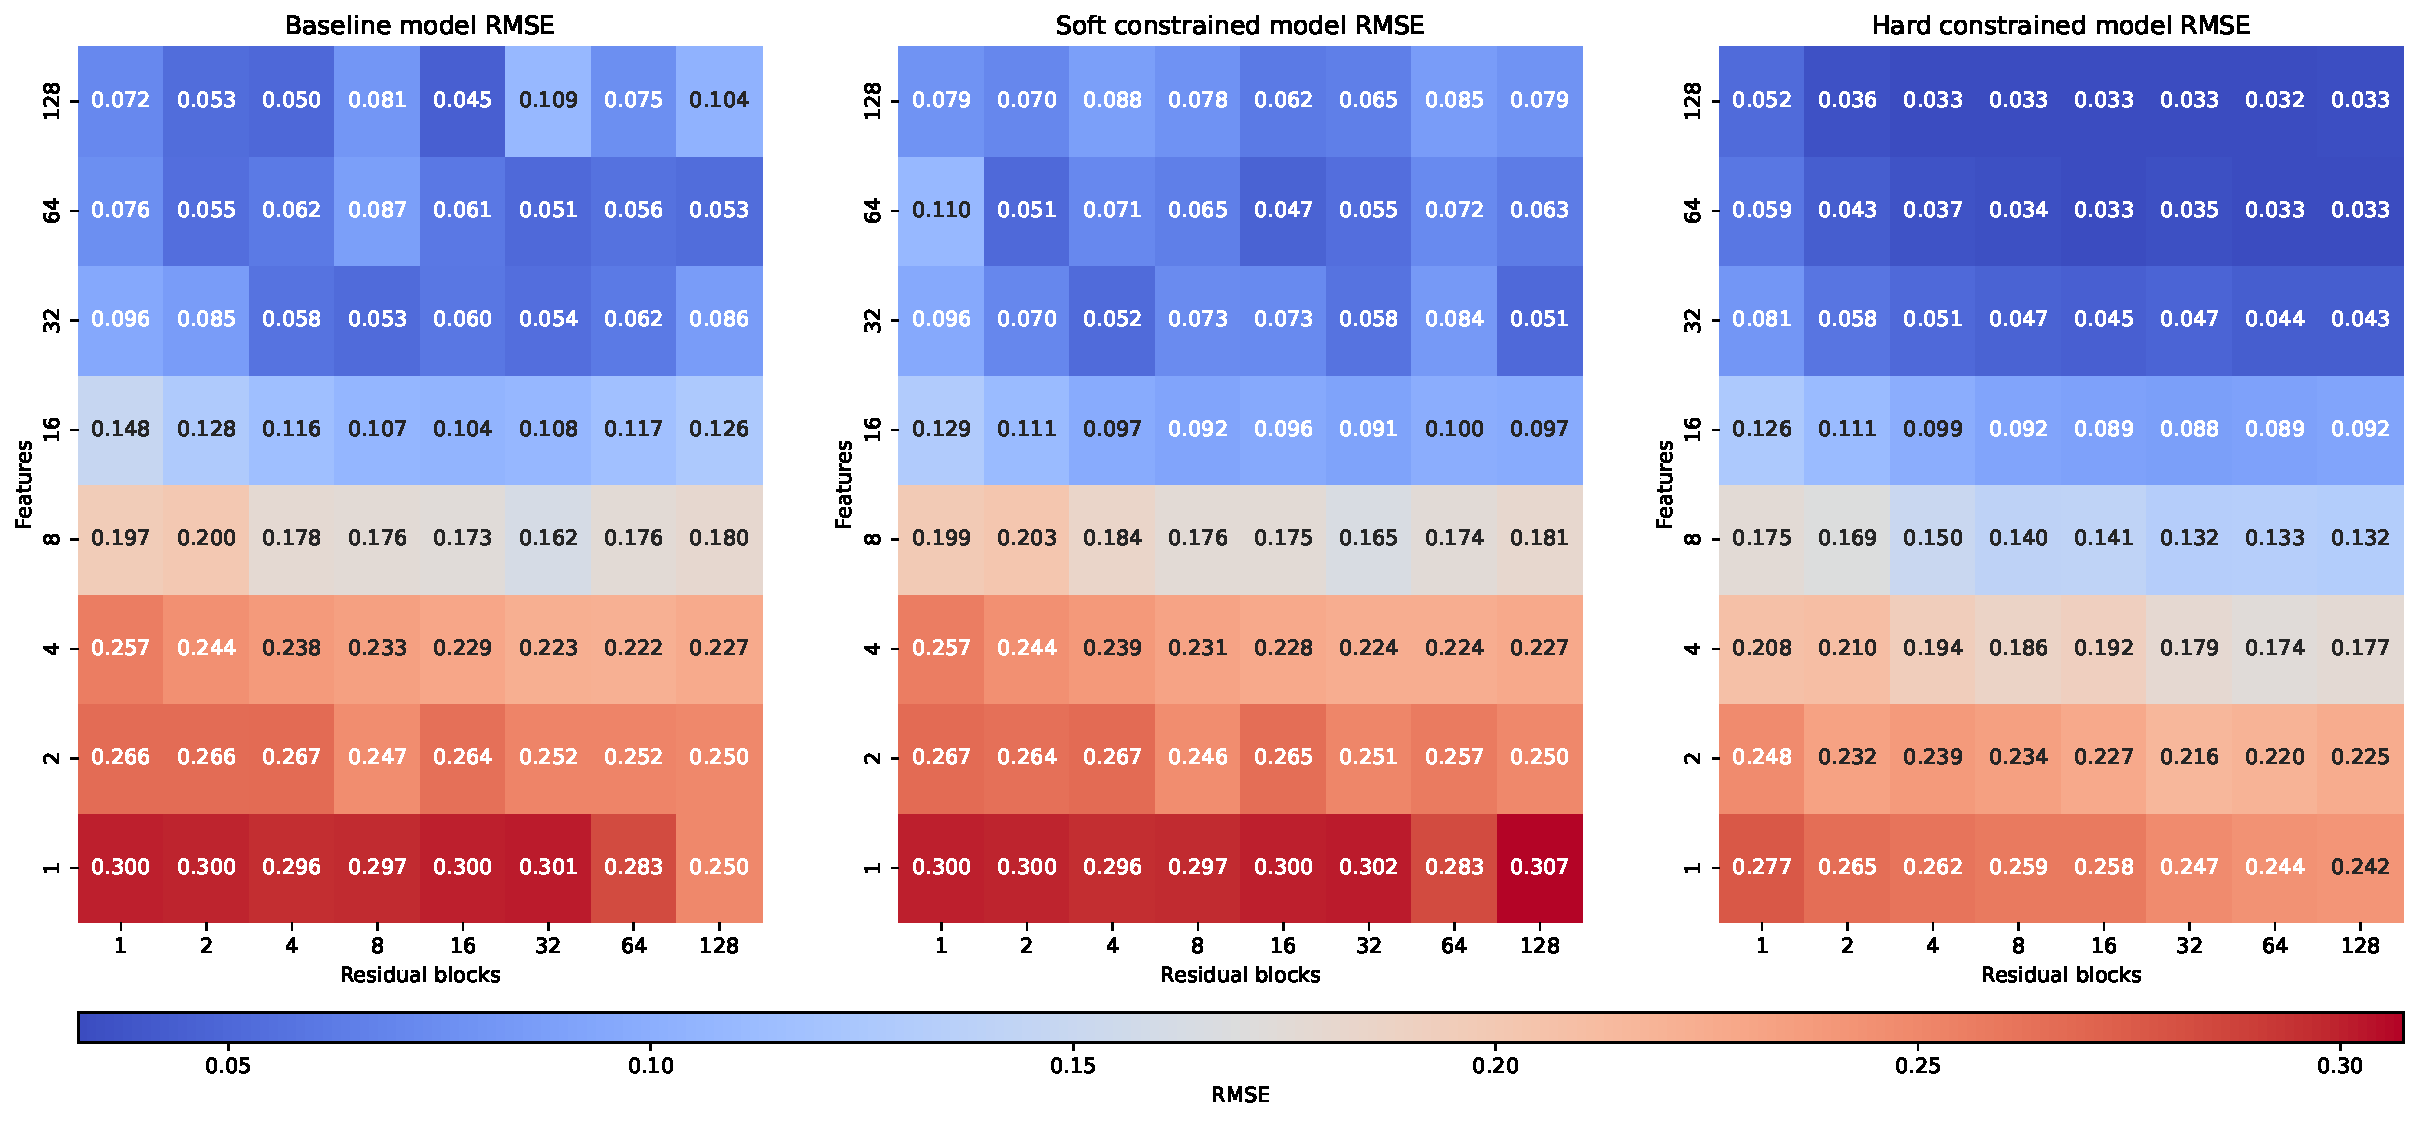
\includegraphics[width=\linewidth]{images/sizes.pdf}
    \caption[Model size experiment]{Model size experiment result. From left to right the RMSEs achieved by unconstrained, soft-constrained and hard-constrained models.}
    \label{fig:sizes}
\end{figure}
\end{landscape}

The absolute differences between the RMSEs of unconstrained models and both soft and hard constrained models are shown in Figure~\ref{fig:sizes_abs_diff}.
For the soft constraint scenario, in the smaller model sizes, the results are comparable to the unconstrained models, except for one case that appears to be random noise.
For the configuration with 16 features, the soft-constrained models consistently yield better performance for every tested number of residual blocks.
Beginning with 32 features and above, the results fluctuate between improvement and deterioration. 
This behavior can be explained by the large pixel-wise error for the small model sizes, forcing the model to focus on that part of the loss function, leading to the same results as the unconstrained models.
For the 16 features, the pixel-wise error drops, and the ratio between it and the constraint violation appears to be ideal.
When the number of features reaches 32 or more, the results for both the unconstrained and soft-constrained models become turbulent. 
This may be due to the low pixel-wise loss, suggesting that the model is overfitted.
On the other hand, the hard constraint scenario shows RMSE improvement across all the model sizes.

\begin{figure}[h]
    \centering
    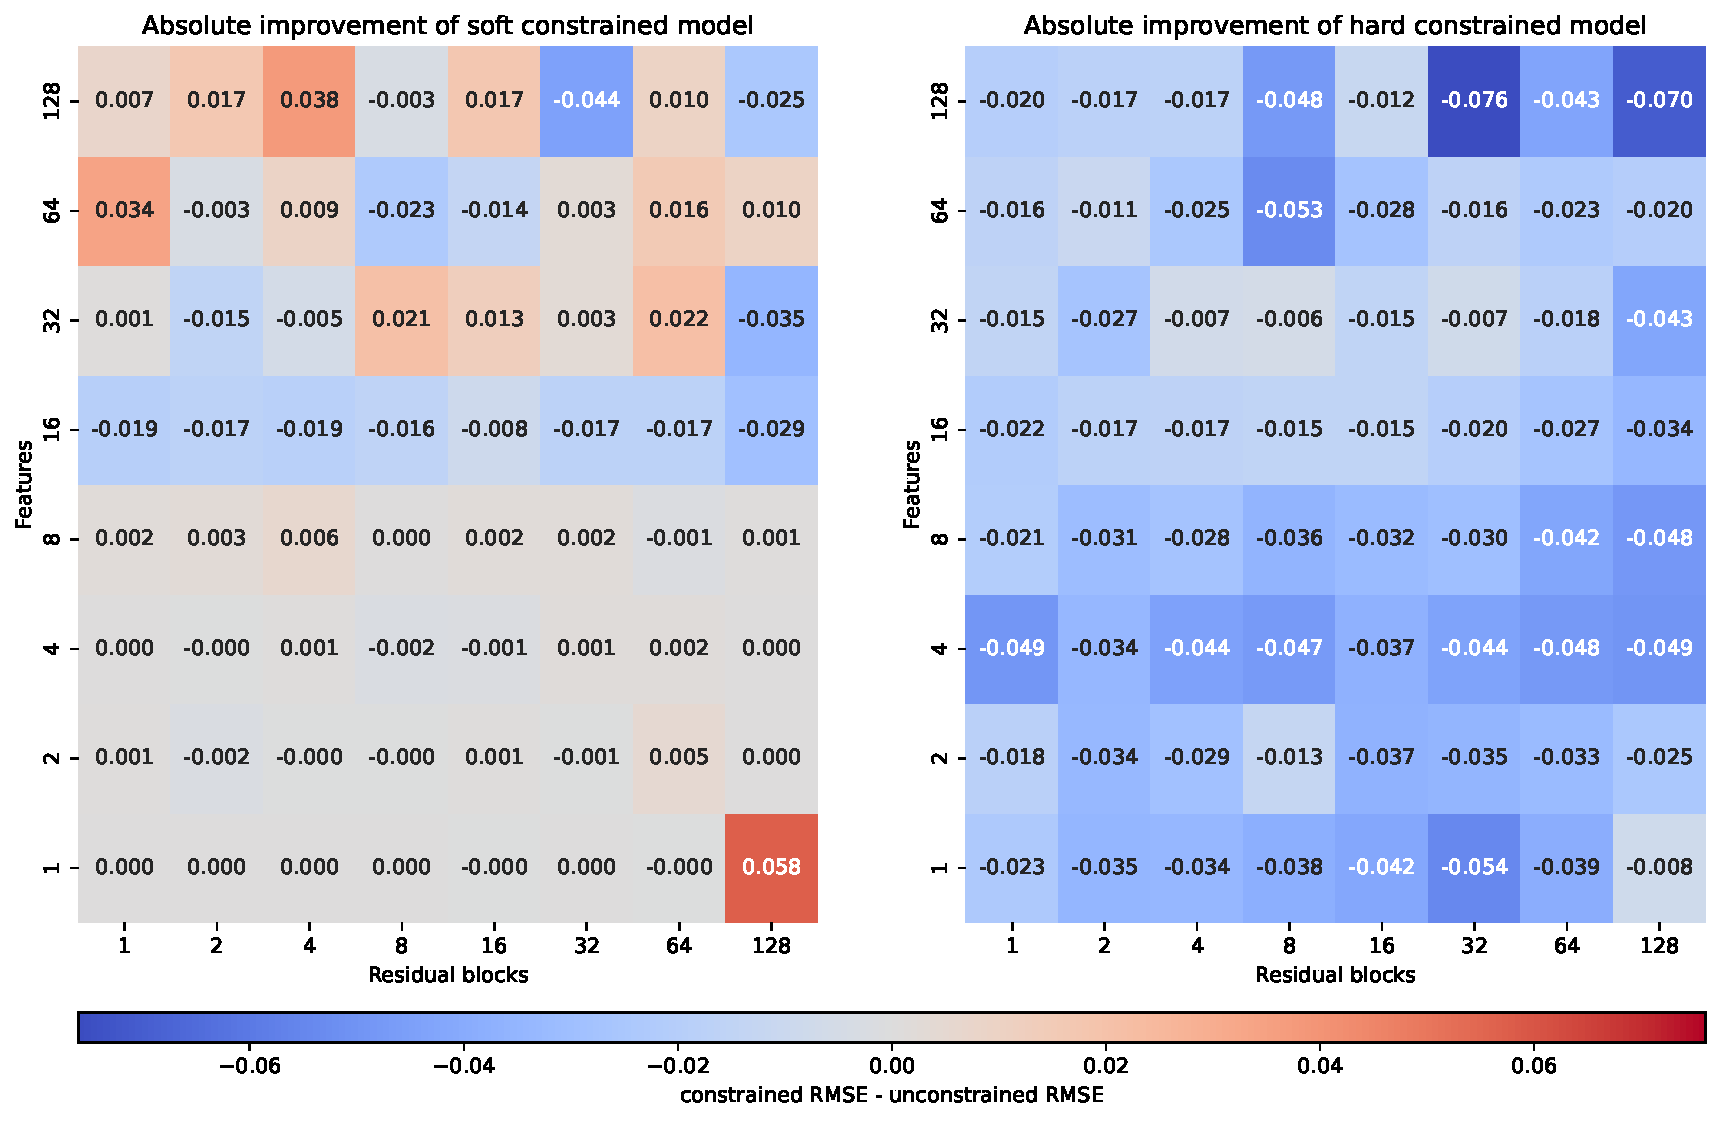
\includegraphics[width=\linewidth]{images/sizes_abs_diff.pdf}
    \caption[Model size experiment -- absolute improvement]{Model size experiment -- absolute improvement. The differences between RMSEs of unconstrained model and soft-constrained (left), resp. hard-constrained (right) models of the same size are shown. When the model's performance improved by incorporating a constraint the value is negative and is displayed in blue, otherwise in red.}
    \label{fig:sizes_abs_diff}
\end{figure}

When focusing on relative improvements (Figure~\ref{fig:sizes_rel_diff}) of the soft and hard constrained models in comparison with their unconstrained counterparts, the conclusions from the previous paragraph remain valid.
Moreover, together with the smoothing effect of the hard constraints shown in Figure~\ref{fig:sizes} and the observation that the relative improvement grows with model size, we conclude that the hard constraint layer contributes to generalization.

\begin{figure}[h]
    \centering
    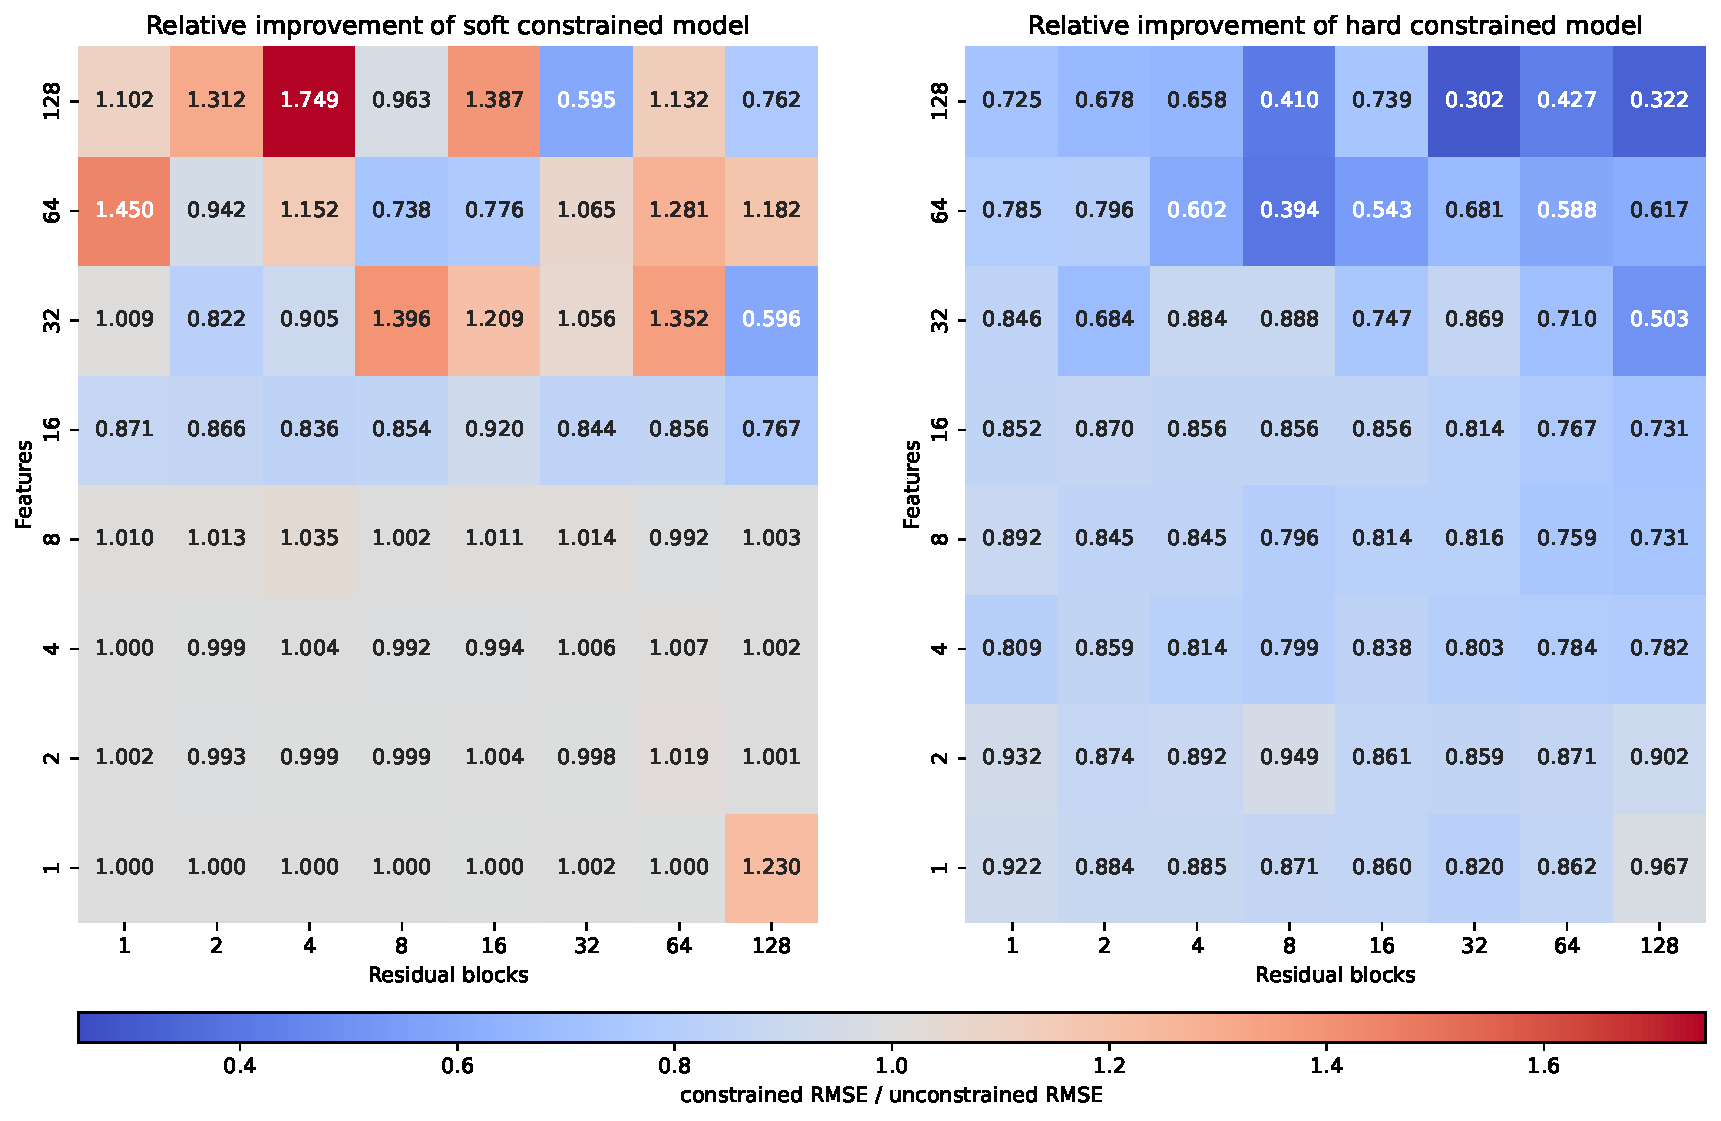
\includegraphics[width=\linewidth]{images/sizes_rel_diff.pdf}
    \caption[Model size experiment -- relative improvement]{Model size experiment -- relative improvement. The ratios between RMSEs of unconstrained model and soft-constrained (left), resp. hard-constrained (right) models of the same size are shown. When the model's performance improved by incorporating a constraint the value is less than one and is displayed in blue, otherwise in red.}
    \label{fig:sizes_rel_diff}
\end{figure}

The lowest RMSE obtained (0.03223) was achieved by the hard-constrained model using 64 residual blocks and 128 features. 
The best performance of the unconstrained model (0.04456) was slightly better than that of the soft-constrained model (0.04702).
That leads us to the conclusion that the hard-constraining layer reduced the pixel-wise error of the unconstrained model by almost 30\%.
Additionally, we observed that the hard-constrained model is dealing more effectively with its size.
In Figure~\ref{fig:sizes_params} we show an example of this observation from the other side.
The lowest RMSE achieved by the unconstrained model is shown by the blue dashed line. 
Reaching this performance requires more than 7.2 million parameters (blue dotted line), while the hard-constrained model needs only about 777 thousand parameters (green dotted line) to outperform the unconstrained model’s best score.
This means adding a constraint layer can improve performance so much that shrinking the model to about one-tenth of its original size does not affect final performance.

\begin{figure}[h]
    \centering
    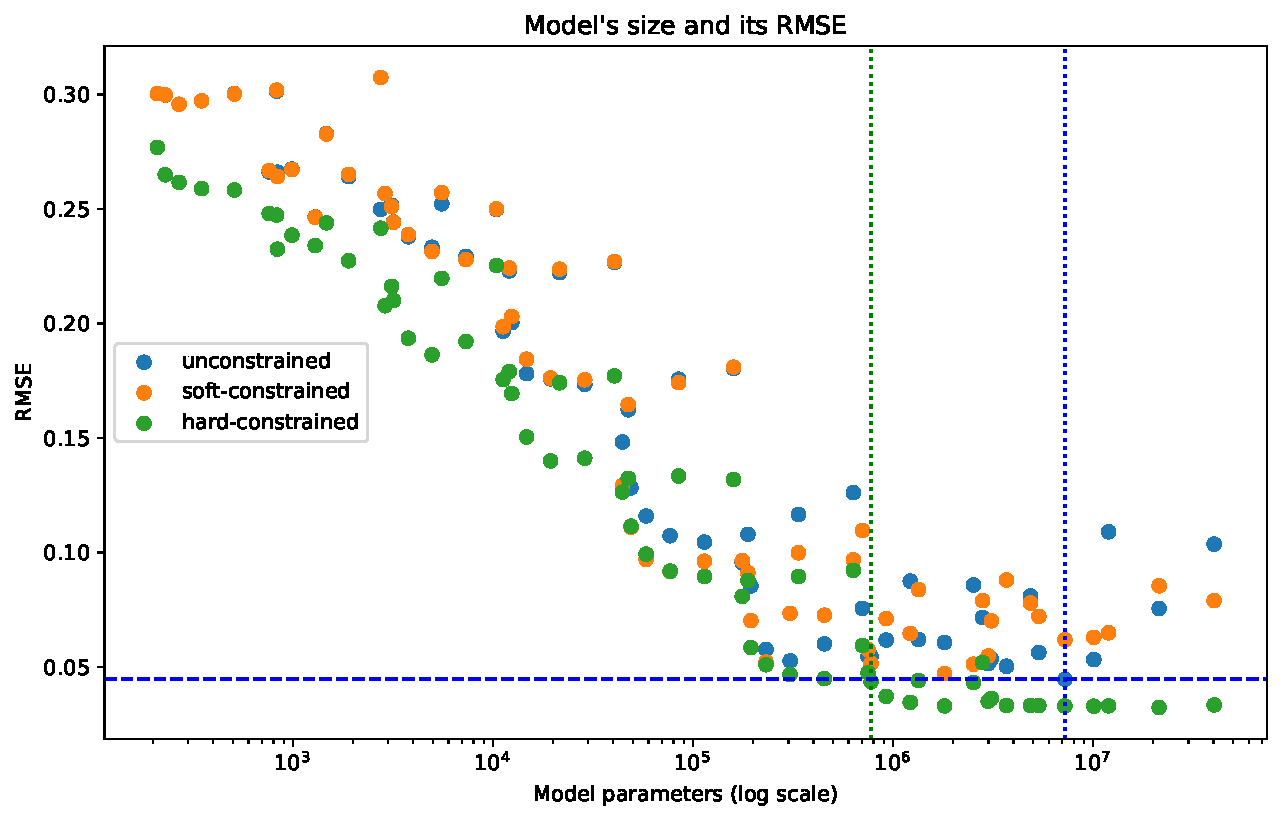
\includegraphics[width=\linewidth]{images/sizes_params.pdf}
    \caption[Model performance and the number of its parameters]{
    Model performance on the validation set and the number of its parameters.
    The lowest RMSE obtained by the unconstrained model is indicated by the blue dashed line, and its corresponding number of parameters is shown by the blue dotted line.
    The hard-constrained model that exceeds this performance while using the fewest learnable parameters is marked with the green dotted line.
    The graph thus suggests that applying a hard constraint can shrink the model size without degrading its performance.}
    \label{fig:sizes_params}
\end{figure}

\section{Evaluation on test data}
\label{s:test_eval}

In the previous experiments, the best improvement resulting from using the constraints was for the scale factor of $16$.
For this scale factor, the best performances on the validation set among the unconstrained, soft-constrained, and hard-constrained models are shown in Table~\ref{tab:val_bests}.

\begin{table}[h!]
    \centering
    \begin{tabular}{|m{0.25\linewidth}|m{0.2\linewidth}|m{0.2\linewidth}|m{0.2\linewidth}|}
        \hline
         \textbf{Model type} & \textbf{Resampling} & \textbf{Validation} \textbf{MAE} & \textbf{Validation} \textbf{RMSE} \\
         \hline \hline
         Unconstrained & cubic spline & 0.02983 & 0.04135 \\
         \hline
         Soft-constrained & average & 0.02709 & 0.0358 \\
         \hline
         Hard-constrained & average & 0.02603 & 0.0315 \\
         \hline
    \end{tabular}
    \caption[Best validation performances for different model types]{
    Best validation performances for different model types. 
    The best performance for the unconstrained model was achieved for the cubic spline resampling, whereas for the constrained models the average performed better. 
    All the best models had 128 features and 64 residual blocks.}
    \label{tab:val_bests}
\end{table}
\newpage
Now, the performance of the models that performed best on the validation set can be evaluated on unseen data from the ReKIS dataset, where we have target HR images.
For the unconstrained, soft-constrained, and hard-constrained models, the test MAE and RMSE metrics are shown in Table~\ref{tab:test_bests}.
We also calculated, for each pixel, the mean absolute error on the test set with the best hard-constrained model (Figure~\ref{fig:test_mae}).
In the referenced figure, the errors do not seem to be uniformly distributed and show a higher number of outliers, which is characteristic of training with absolute error.
A greater proportion of pixels showing higher mean absolute errors is found in the mountainous areas, where temperature downscaling is more challenging.
However, these pixels do not constitute a larger area and can be regarded as localized phenomena.

\begin{table}[h]
    \centering
    \begin{tabular}{|m{0.25\linewidth}|m{0.2\linewidth}|m{0.2\linewidth}|m{0.2\linewidth}|}
        \hline
         \textbf{Model type} & \textbf{Resampling} & \textbf{Test} \textbf{MAE} & \textbf{Test} \textbf{RMSE} \\
         \hline \hline
         Unconstrained & cubic spline & 0.02929 & 0.03886 \\
         \hline
         Soft-constrained & average & 0.02667 & 0.0338 \\
         \hline
         Hard-constrained & average & 0.02575 & 0.0306 \\
         \hline
    \end{tabular}
    \caption[Best test performances for different model types]{Best test performances for different model types. The best is the hard-constrained model. It is important to note that these models are the same as in Table~\ref{tab:val_bests}, only here the performance on test set is shown.}
    \label{tab:test_bests}
\end{table}

\begin{figure}[h]
    \centering
    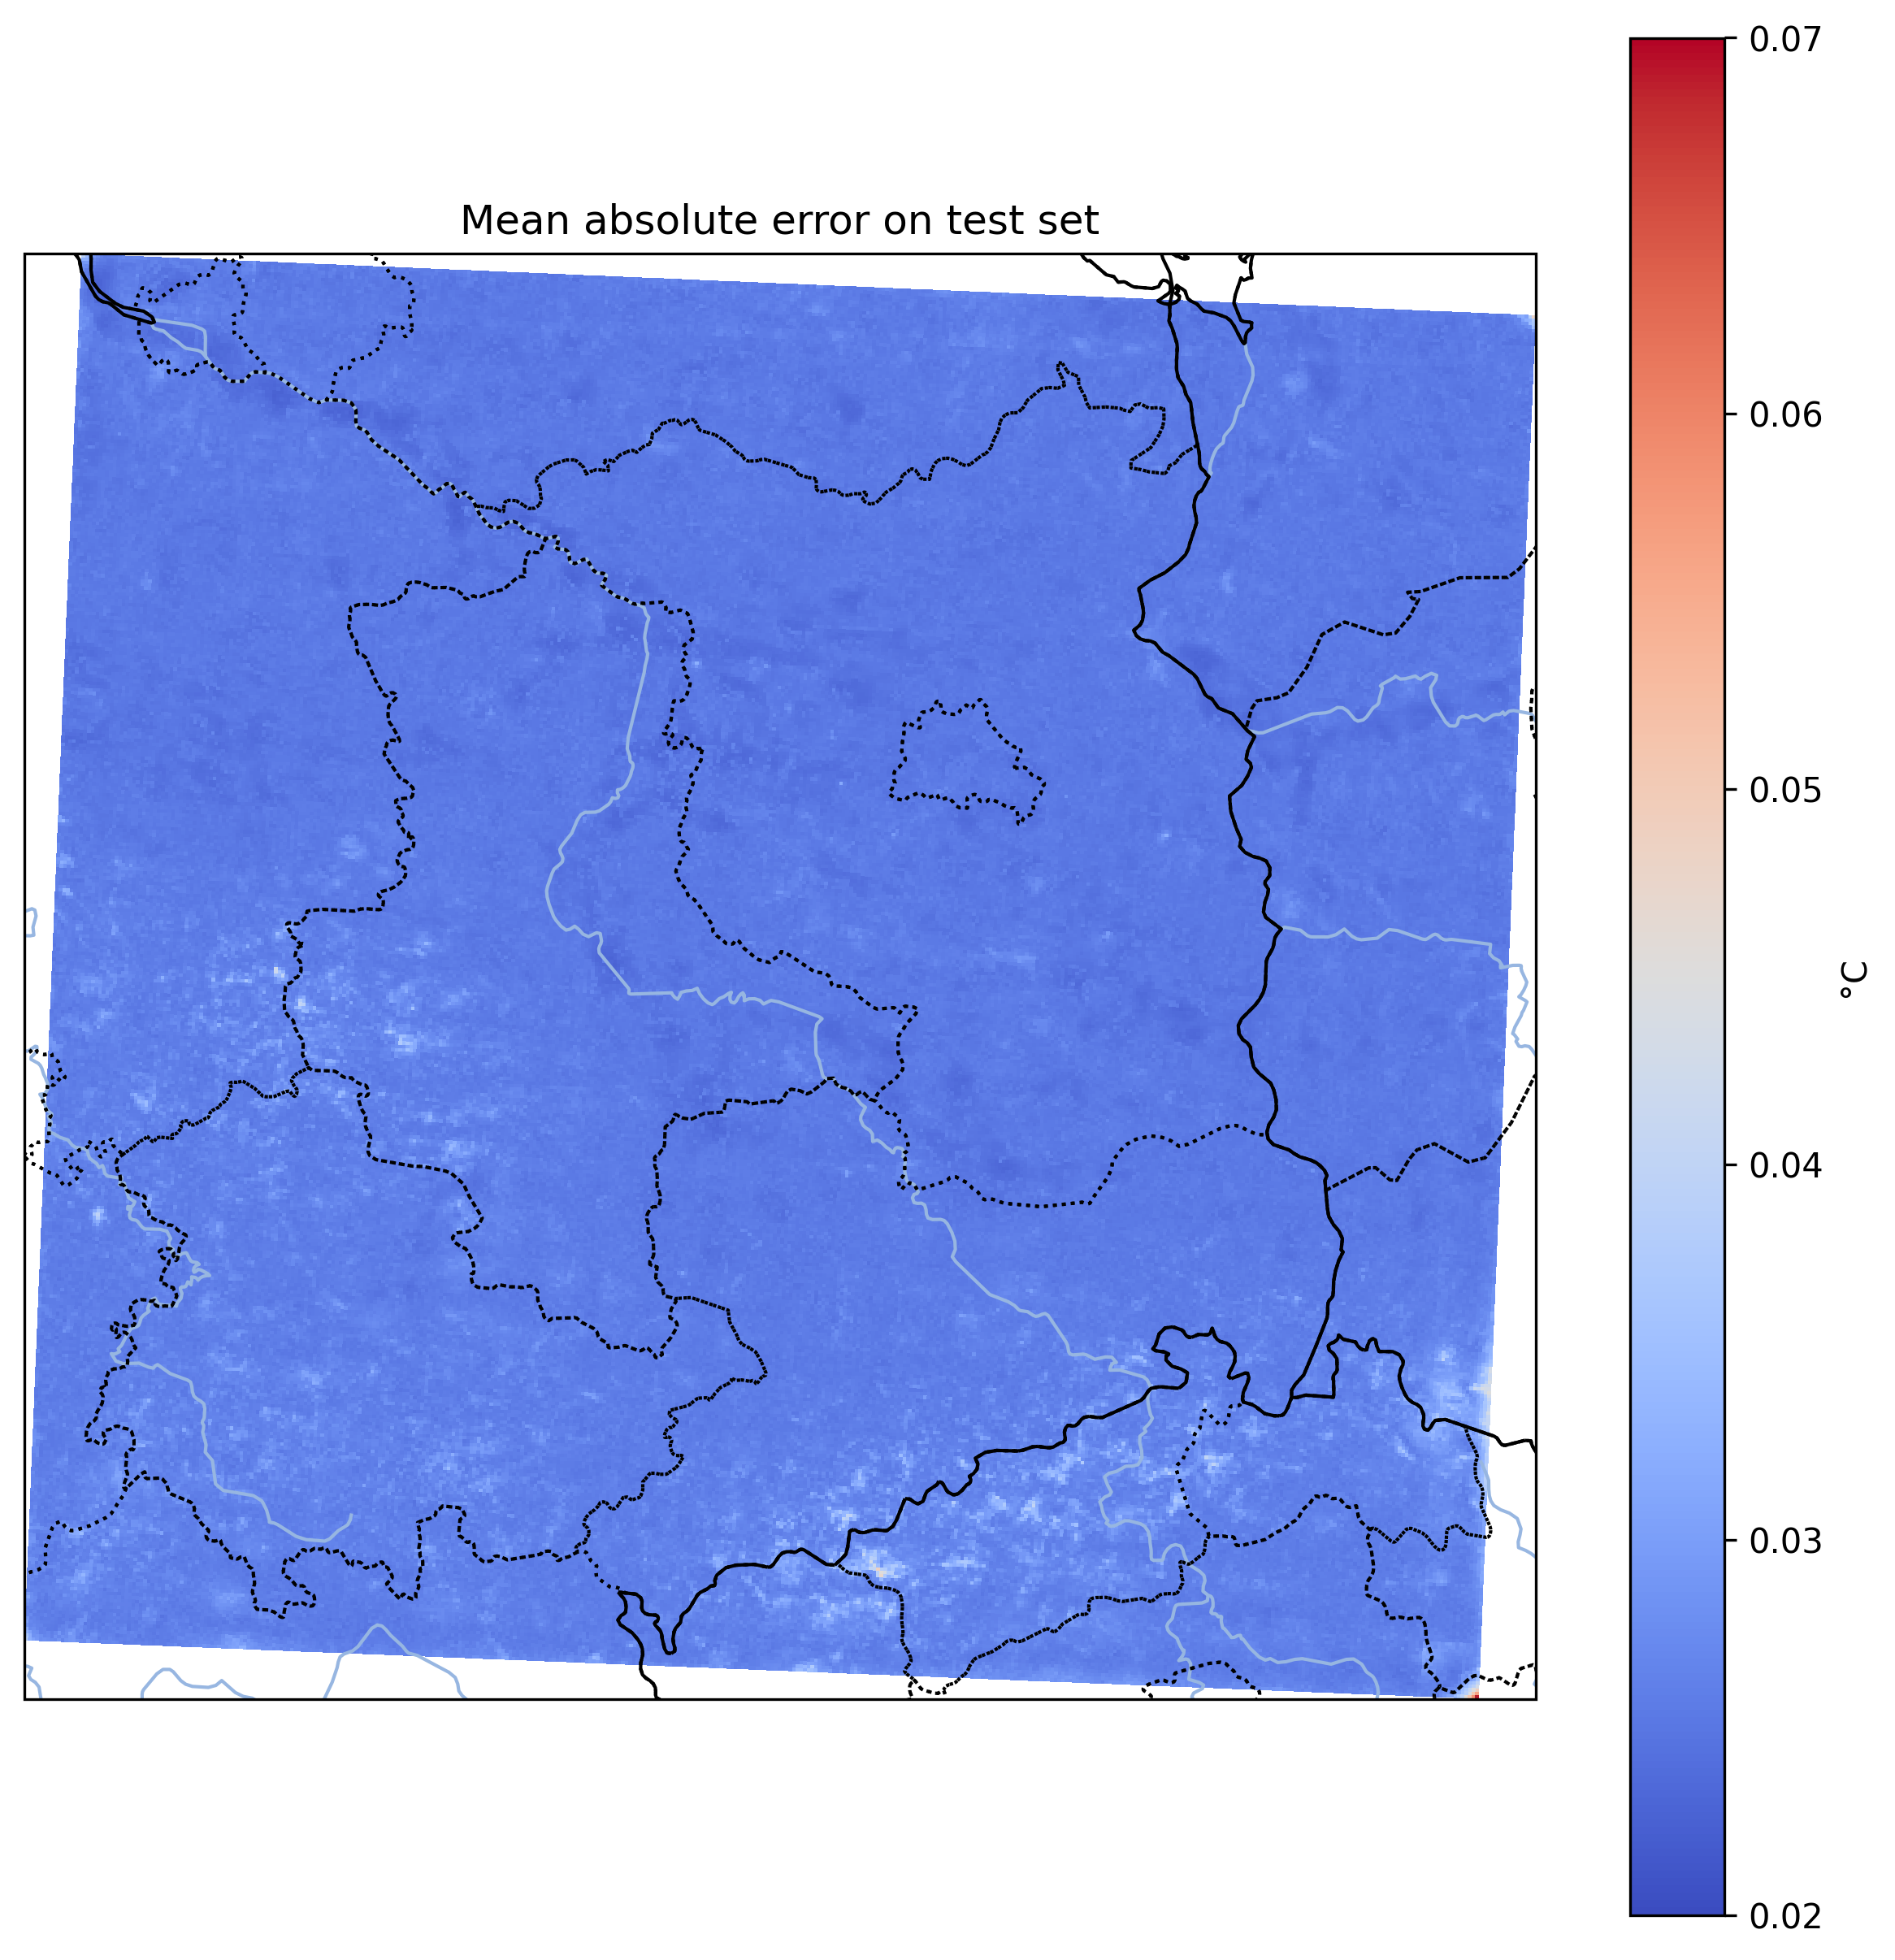
\includegraphics[width=0.5\linewidth]{images/mae.png}
    \caption[MAE on test set for the best model]{MAE on test set for the best model. The errors are not spread uniformly; only certain pixels exhibit large errors -- a characteristic pattern when training with an absolute-error loss function. The pixels that pose the greatest challenges for the model are found in the mountainous areas rather than in the plains.}
    \label{fig:test_mae}
\end{figure}

\section{Downscaling of EURO-CORDEX}

The best performance was measured (Section~\ref{s:test_eval}) in the setup of average resampling and the hard-constrained EDSR with 128 features and 64 residual blocks.
The EURO-CORDEX data must be reprojected to align with the CRS and resolution of the LR ReKIS data before being fed into the neural network.
After this procedure, they were downscaled using the above defined model.
The results are shown as visual examples in Figure~\ref{fig:downscaled_cordex}.
However, we are unable to further evaluate these results because no high-resolution EURO-CORDEX data are available.

\begin{figure}
    \centering
    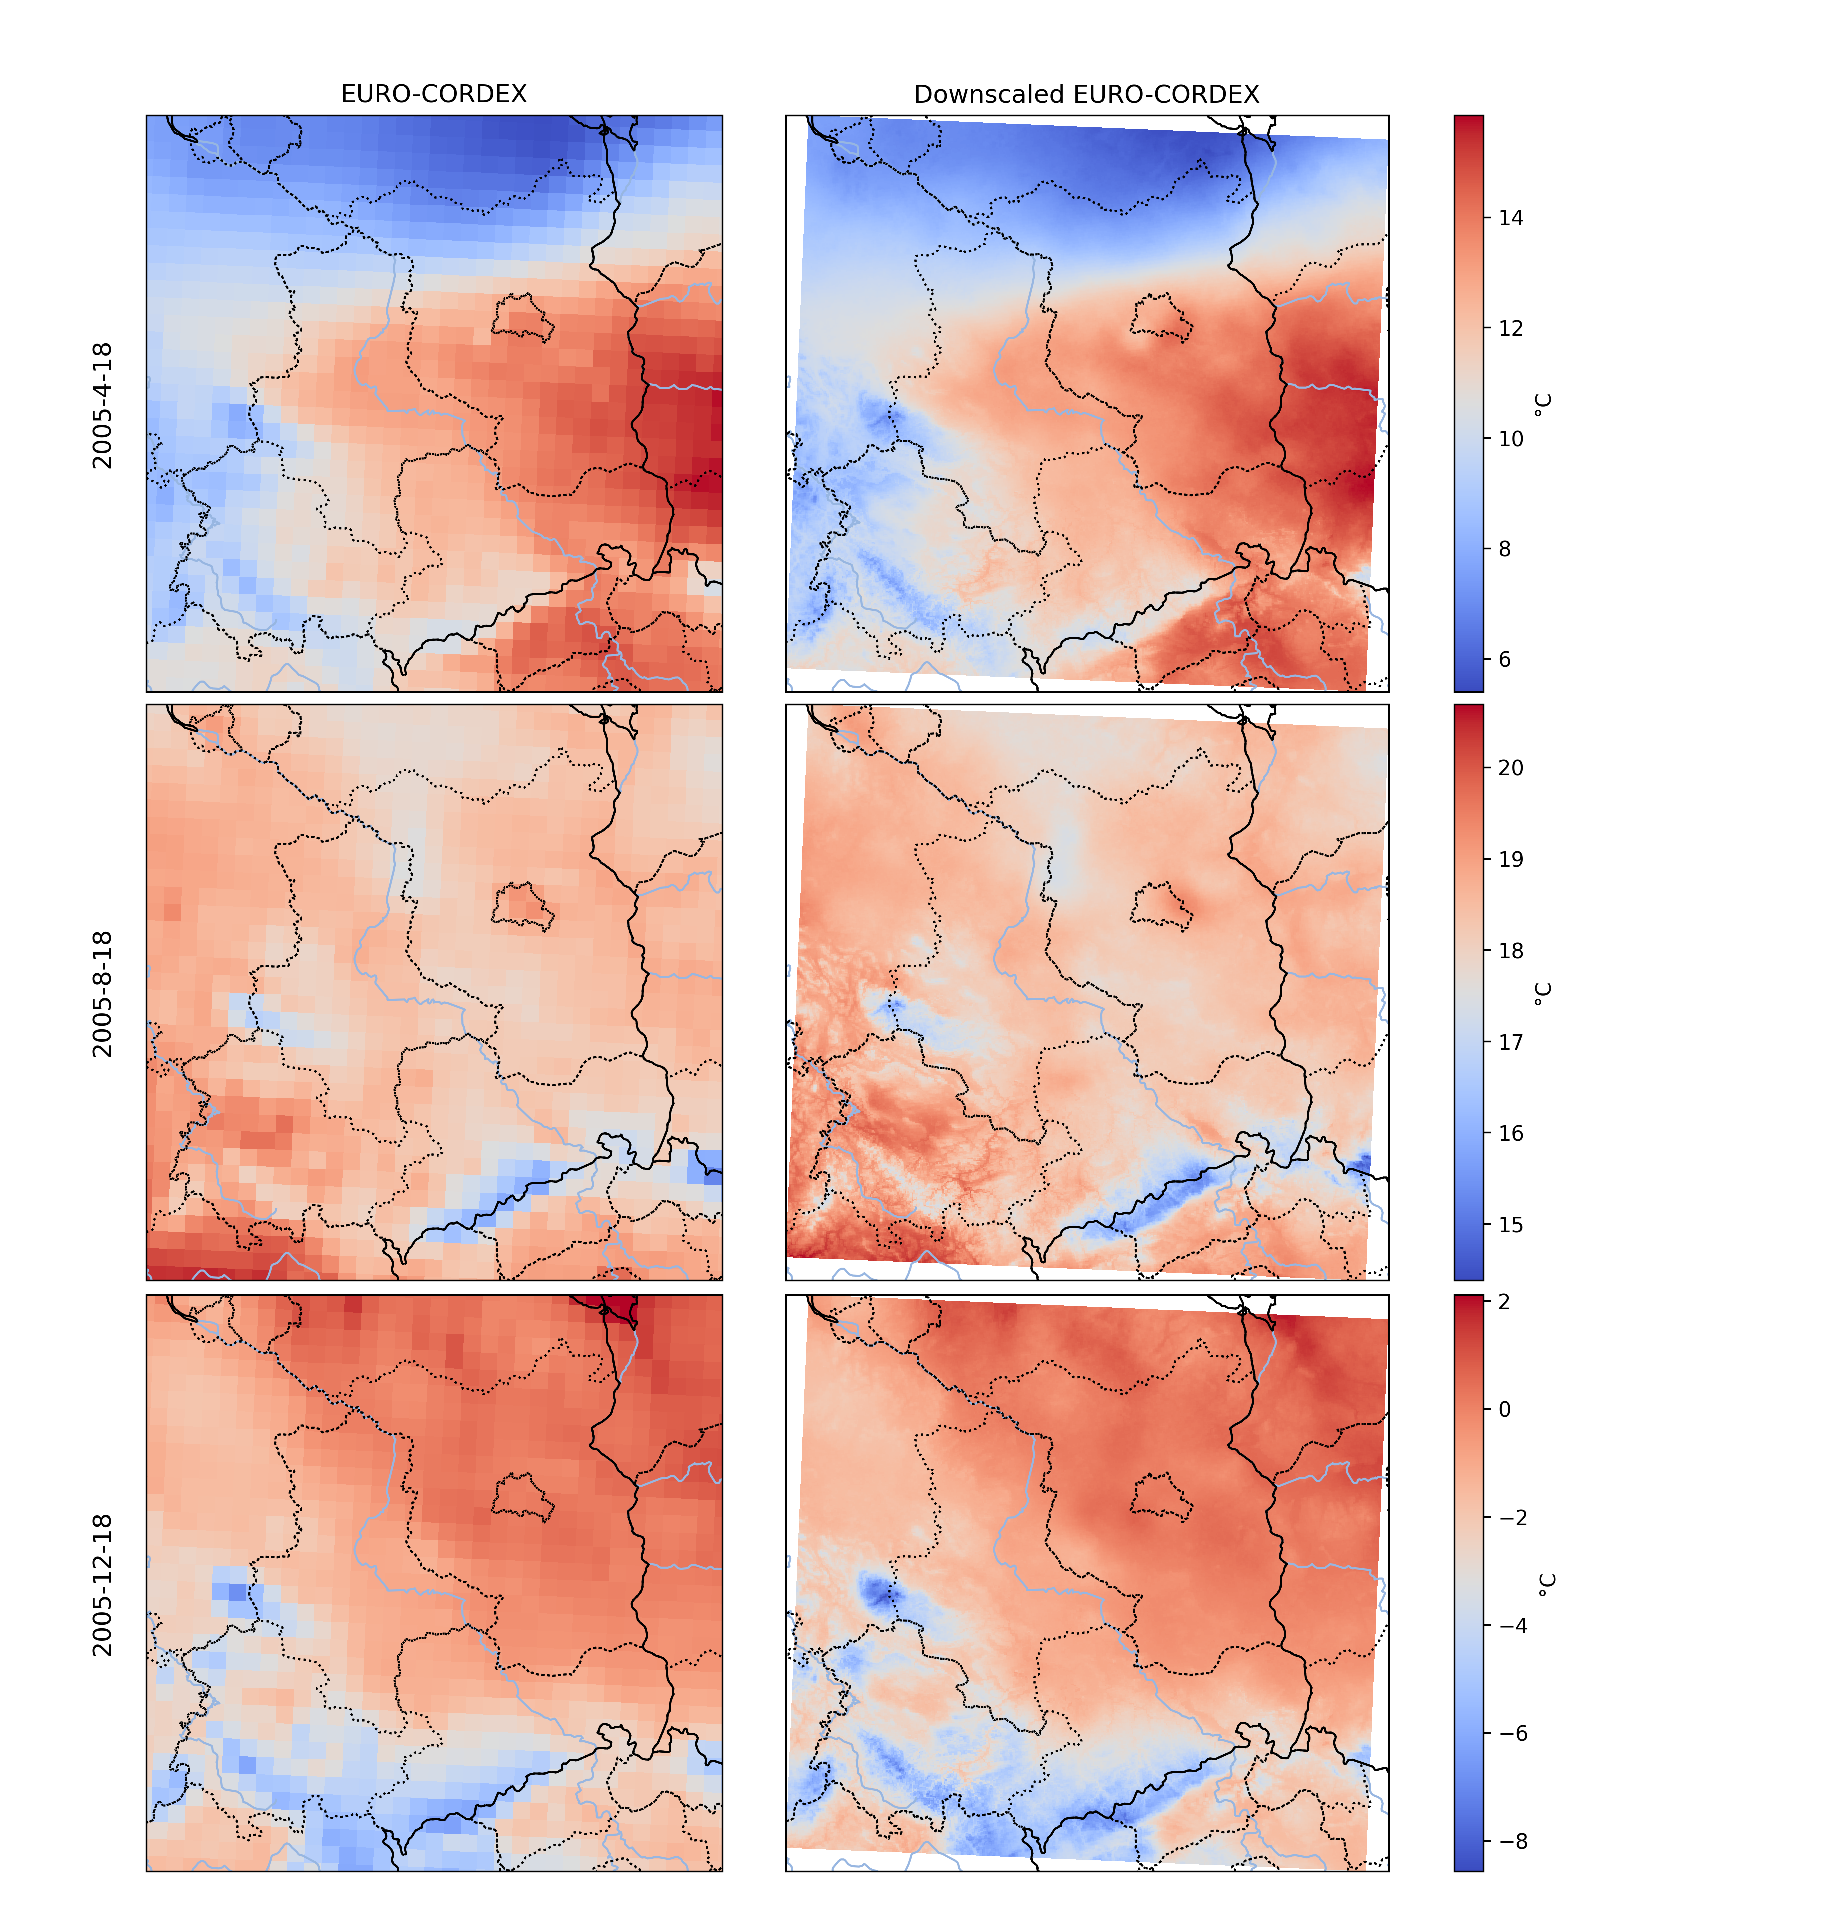
\includegraphics[width=\linewidth]{images/downscaled_cordex.pdf}
    \caption[Downscaling EURO-CORDEX]{
    Downscaling EURO-CORDEX. 
    On the left, images from the original resolution of EURO-CORDEX dataset are shown in the study region. 
    They are then upscaled so they can be used as input to our model, producing the images displayed on the right.
    The images are shown in distinct seasons.
    In April we can see a smooth transition from cold on the north to warmer weather in the central part of the region, which is smoother in the downscaled version.
    Across all displayed images, high-resolution features are mainly visible in the mountainous area in the southeastern part of the region and along the German-Czech border.
    Note that on the left, the EURO-CORDEX data cover all of Europe, while the downscaled dataset is limited to the ReKIS region, which results in the white areas along the sides.
    }
    \label{fig:downscaled_cordex}
\end{figure}


%---------------------------------------------------------------
\chapter{Discussion}
%---------------------------------------------------------------

In the study by Harder et al.~\cite{Harder2023}, the hard-constrained model outperformed the unconstrained model when moist static energy conservation was enforced in downscaling the water content and temperature.
In the same work, the same conservation law was also imposed on natural images, where it has no physical meaning. 
Yet, it again yielded better results than the unconstrained model.
In contrast, when the conservation constraint was applied only to temperature in the NorESM dataset, the constrained models did not surpass the unconstrained baseline.
It is important to note that temperature alone cannot be integrated, and the additional variables needed to compute moist static energy are not available.
Consequently, this configuration also lacks a solid physical basis.
Our improved performance (Section~\ref{s:test_eval}) in a comparable setting -- downscaling temperature with the conservation constraint applied solely to temperature -- can be explained by the following factors:
\begin{description}
    \item[Resampling method.]  
    Harder et al.~\cite{Harder2023} reported substantial violations of the assumed constraint between their LR and HR data, in part because the LR data were not obtained by resampling the HR; instead, they originated from the same source at different resolutions.
    We likewise quantified these violations for different resampling schemes and tested two of them.
    With average resampling, the violations in the LR–HR pairs were almost negligible, and the constraints improved the model’s performance.
    In contrast, using cubic spline resampling led to large violations in the LR–HR pairs, and incorporating the constraints did not produce a significant benefit.
    \item[Scale factor.]
    While Harder et al.~\cite{Harder2023} adopted a scale factor of 2, we experimented with them and found that the largest improvement is for 16.
    Over the range of scale factors considered, the relative improvement remained small for low scale factors, where the task appears too simple, and for very high scale factors, where the LR image comprises only a few pixels and the reconstruction problem becomes extremely difficult.
    \newpage
    \item[Resolution.]
    In Harder et al.~\cite{Harder2023}, the LR and HR grids had resolutions of $2^\circ$ and $1^\circ$ (around 200 and 100 km), respectively, whereas in our case, for a scale factor of 16, the corresponding resolutions are approximately $0.16^\circ$ and $0.01^\circ$ (16 and 1 km).
    We regard this discrepancy as substantial and hypothesize that resolution contributes to the differing outcomes, since temperature variability is clearly greater over a $200\times 200$ km area than over a $16\times 16$ km region.
\end{description}



%---------------------------------------------------------------
\chapter{Conclusion}
%---------------------------------------------------------------

In Chapter~\ref{ch:related_work}, we focused on describing the current state of research. 
It has been discussed that the models and datasets have been recently applied to both climate and non-climate downscaling. 
The problem of physical consistency has also been emphasized, and several proposed solutions have been reviewed and summarized.
We also emphasized that physical constraints can involve more than one physical quantity.
Moreover, the necessary theoretical pillars of our work have been defined, such as the concepts of neural networks, evaluation metrics, vector fields, and image processing.
We presented the used neural network architecture -- EDSR. 
However, the main emphasis was on defining the constraints.
We have proposed a more general definition than in Harder et al.~\cite{Harder2023}.
We introduced the concept of the dilated derivative and demonstrated its consistency under downscaling.
Following Harder et al.~\cite{Harder2023}, the same conservation law has been adopted, applying it both as a soft and a hard constraint.
In addition, we adapted several physical loss function augmentations so that they satisfy the formal definition of a constraint and incorporated them as soft constraints.
All these constraints were built upon the principle of dilated derivative consistency.

In Chapter~\ref{ch:experiments},  the introduction of the observational gridded dataset used for model training -- ReKIS -- as well as the climate projection dataset -- EURO-CORDEX -- took place.
After that, the data preprocessing specification followed.
We have also conducted more experiments on the ReKIS dataset aimed at identifying the most suitable configuration of the resampling technique, scale factor, constraint type, and their specific settings (alpha value for the soft-constraint approach, and constraining layer type for the hard-constraint approach).
These experiments were carried out with the goal of determining the optimal setup for downscaling EURO-CORDEX.

In Section~\ref{s:resampling_method_exp}, we showed that the chosen resampling method used to generate the LR images substantially affects the model’s performance, with a particularly strong effect in the hard-constraint setting.
In addition, the introduction of constraints -- both soft and hard -- generally improved the models’ metrics across almost all scale factors.
The most pronounced gain, however, occurred at a scale factor of 16.
We also demonstrated that the constraints themselves are sensitive to the resampling method, as all of them detect some level of violation when applied to HR–LR image pairs, except in the case where the LR images are obtained via average pooling of the HR images.

We tested all soft constraints on ReKIS using two penalty formulations for constraint violations -- absolute and squared in Section~\ref{s:constraints_exp}.
All tested constraints produced meaningful effects; however, the constraint based on the difference between simple derivatives with respect to both coordinates turned out to be the most effective.

Consequently, we conducted experiments (Section~\ref{s:soft_constraints_alpha_exp}) varying the relative weight of the constraint term with respect to the pixel-wise loss.
Performance improved when the pixel-wise term dominated the loss.
The optimal value of $\alpha$ -- the weighting factor of the constraint loss -- matched the value reported by Harder et al.~\cite{Harder2023}, namely $10^{-4}$.

Finally, in Section~\ref{s:models_size_exp}, we investigated the impact of model size.
We ran experiments with unconstrained, soft-constrained, and hard-constrained EDSR models, varying both the number of residual blocks and the number of channels used in them.
Across all runs, the hard-constrained model consistently delivered superior performance.
In one configuration, it even reduced the pixel-wise error to one third of that obtained by an unconstrained model of the same size.
In addition, we observed markedly improved stability in the performance of hard-constrained models as the model size increased.

\section{Future work}

This work has demonstrated the beneficial impact of applying physical constraints to mean temperature downscaling across different EDSR model sizes and scale factors. 
However, no experiments were carried out for other physical variables. 
Consequently, assessing how far these physical constraints can be extended to additional quantities remains an avenue for future research. 
In addition, multiple variables could be downscaled simultaneously -- multivariate downscaling -- where the constraints could be exploited to enforce specific physical relationships among the variables. 
Additionally, introducing further physical constraints that depend only on temperature could enhance the performance of the current model.

Throughout this study, only the EDSR architecture was used; other models, such as SwinIR, which achieved the best performance in Košťál et al.~\cite{Kostal2025}, could also be explored. 
Moreover, a broader exploration of resampling methods, scale factors, model architectures, model sizes, constraint formulations, alpha settings, and additional configurations could reveal a model with superior performance.
\newpage
ReKIS was the sole dataset used in this work for training and evaluating the proposed models and methods. 
Incorporating other data sources could improve the generalization capability of the models.
Moreover, ReKIS's area is dominated by plains, that can be recognized by the relatively large scale factors and small error values in this work; however, focusing on a more mountainous region could identify limitations of the configuration used in this work.

\subsubsection*{Acknowledgment}

The access to the computational infrastructure of the OP VVV funded project CZ.02.1.01/0.0/0.0/16\_019/0000765 ``Research Center for Informatics'' is also gratefully acknowledged.


% \include{text/text} % include `text.tex' from `text/' subdirectory

\appendix\appendixinit % do not remove these two commands

\chapter{Training details}

All experiments were carried out on the RCI (Research Center for Informatics) Cluster at the Czech Technical University in Prague.

Following Košťál et al.~\cite{Kostal2025}, we used the Adam optimizer with a learning rate $10^{-4}$ and a weight decay penalty of $10^{-5}$.
The only alternative learning rate employed was $2\cdot 10^{-4}$, used for the hard-constrained models in the resampling experiments (Section~\ref{s:resampling_method_exp}). 
This choice was made because the hard-constrained models exhibit a very smooth learning curve, whereas the other models are far less stable, making the higher learning rate unsuitable for them (see Figure\ref{fig:validation_rmse}).
Furthermore, an early stopping strategy with a patience of 15 was applied based on the validation pixel-wise RMSE, except in the experiment on model sizes (Section~\ref{s:models_size_exp}), where the patience was reduced to 10, due to the larger number of runs.

\begin{figure}[h]
    \centering
    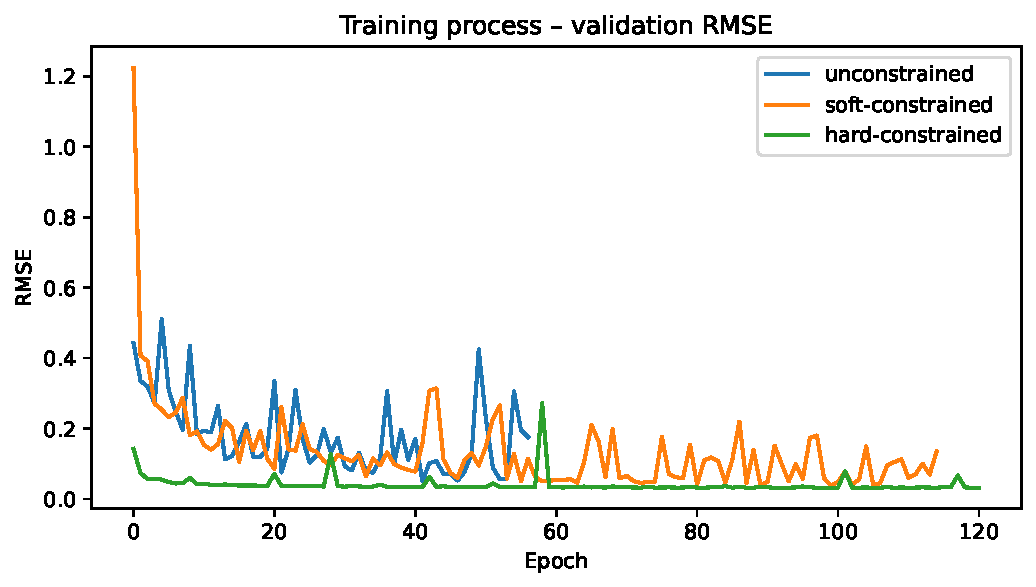
\includegraphics[width=0.7\linewidth]{images/validation_rmse.pdf}
    \caption[Training process]{Training process. 
    An unconstrained a conservation soft-constrained and a conservation hard-constrained models validation pixel-wise RMSEs are shown through the learning process. 
    All the models are EDSR with 128 features and 64 residual blocks. 
    The unconstrained and the soft-constrained model have Adam optimizer with the learning rate of $10^{-4}$, whereas the hard-constrained model has $2\cdot 10^{-4}$, yet it appears to be more stable through the learning.}
    \label{fig:validation_rmse}
\end{figure}

\chapter{Image comparisons}

In Chapter~\ref{ch:experiments} various experiments have been concluded on ReKIS data.
However, only a numerical evaluation of the employed models took place via MAE or RMSE metrics.
Now we present the visual distinctions between the selected models.
In every visualization, the LR model input and the corresponding HR target are displayed.
First, the entire area is shown, followed by a blue square highlighting a zone where elevation, and thus the temperature, are steadier.
Lastly, the red square marks an area characterized by strong temperature variations.

\begin{landscape}
    \begin{figure}
    \centering
    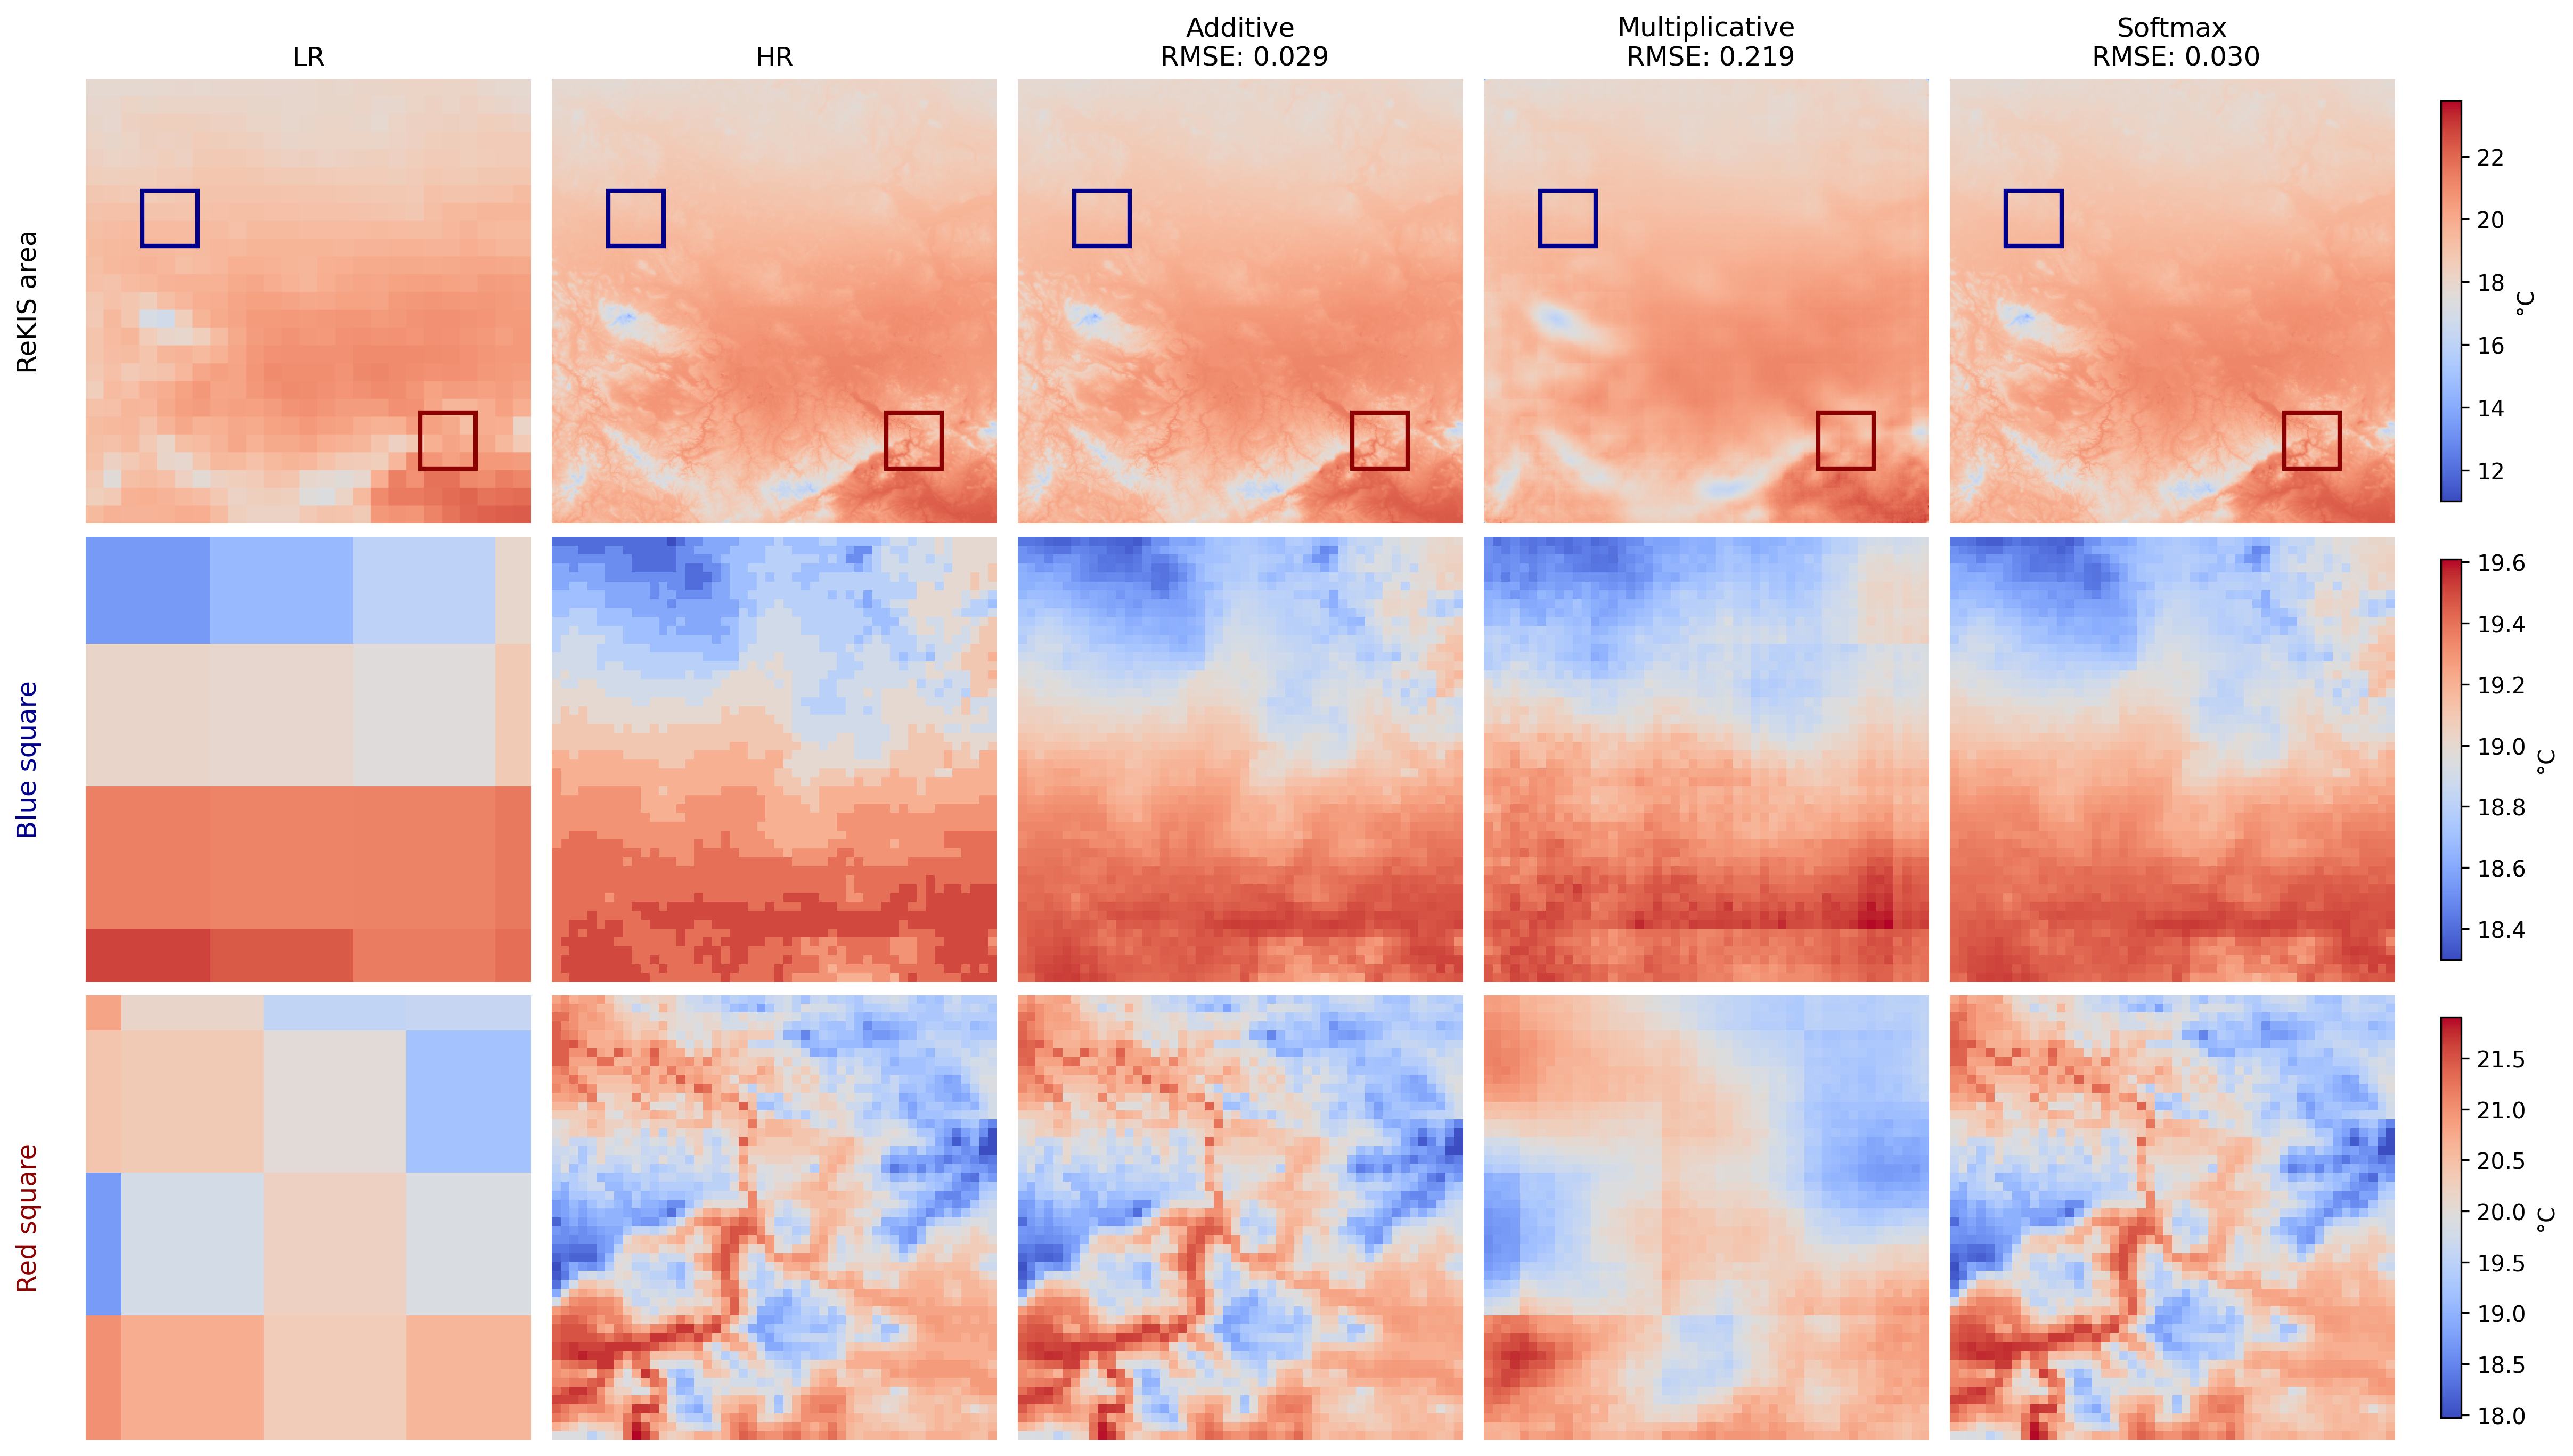
\includegraphics[width=0.88\linewidth]{images/hard_types_comp.png}
    \caption[Hard-constrained model types -- output visual comparison]{
    Hard-constrained model types -- output visual comparison. 
    The models are from Section~\ref{s:hard_constraint_exp}. 
    The multiplicative hard-constraint layer is significantly different than the other implementations -- the larger LR pixels are visible in the blurred output. 
    The HR image in the blue square displays artifacts that look as if it has been rounded or truncated to a fixed number of decimal places. 
    The additive and the softmax approaches are almost identical.
    Images correspond to the date 2005-08-18.}
    \label{fig:hard_types_comp}
\end{figure}
\end{landscape}

\begin{landscape}
    \begin{figure}
        \centering
        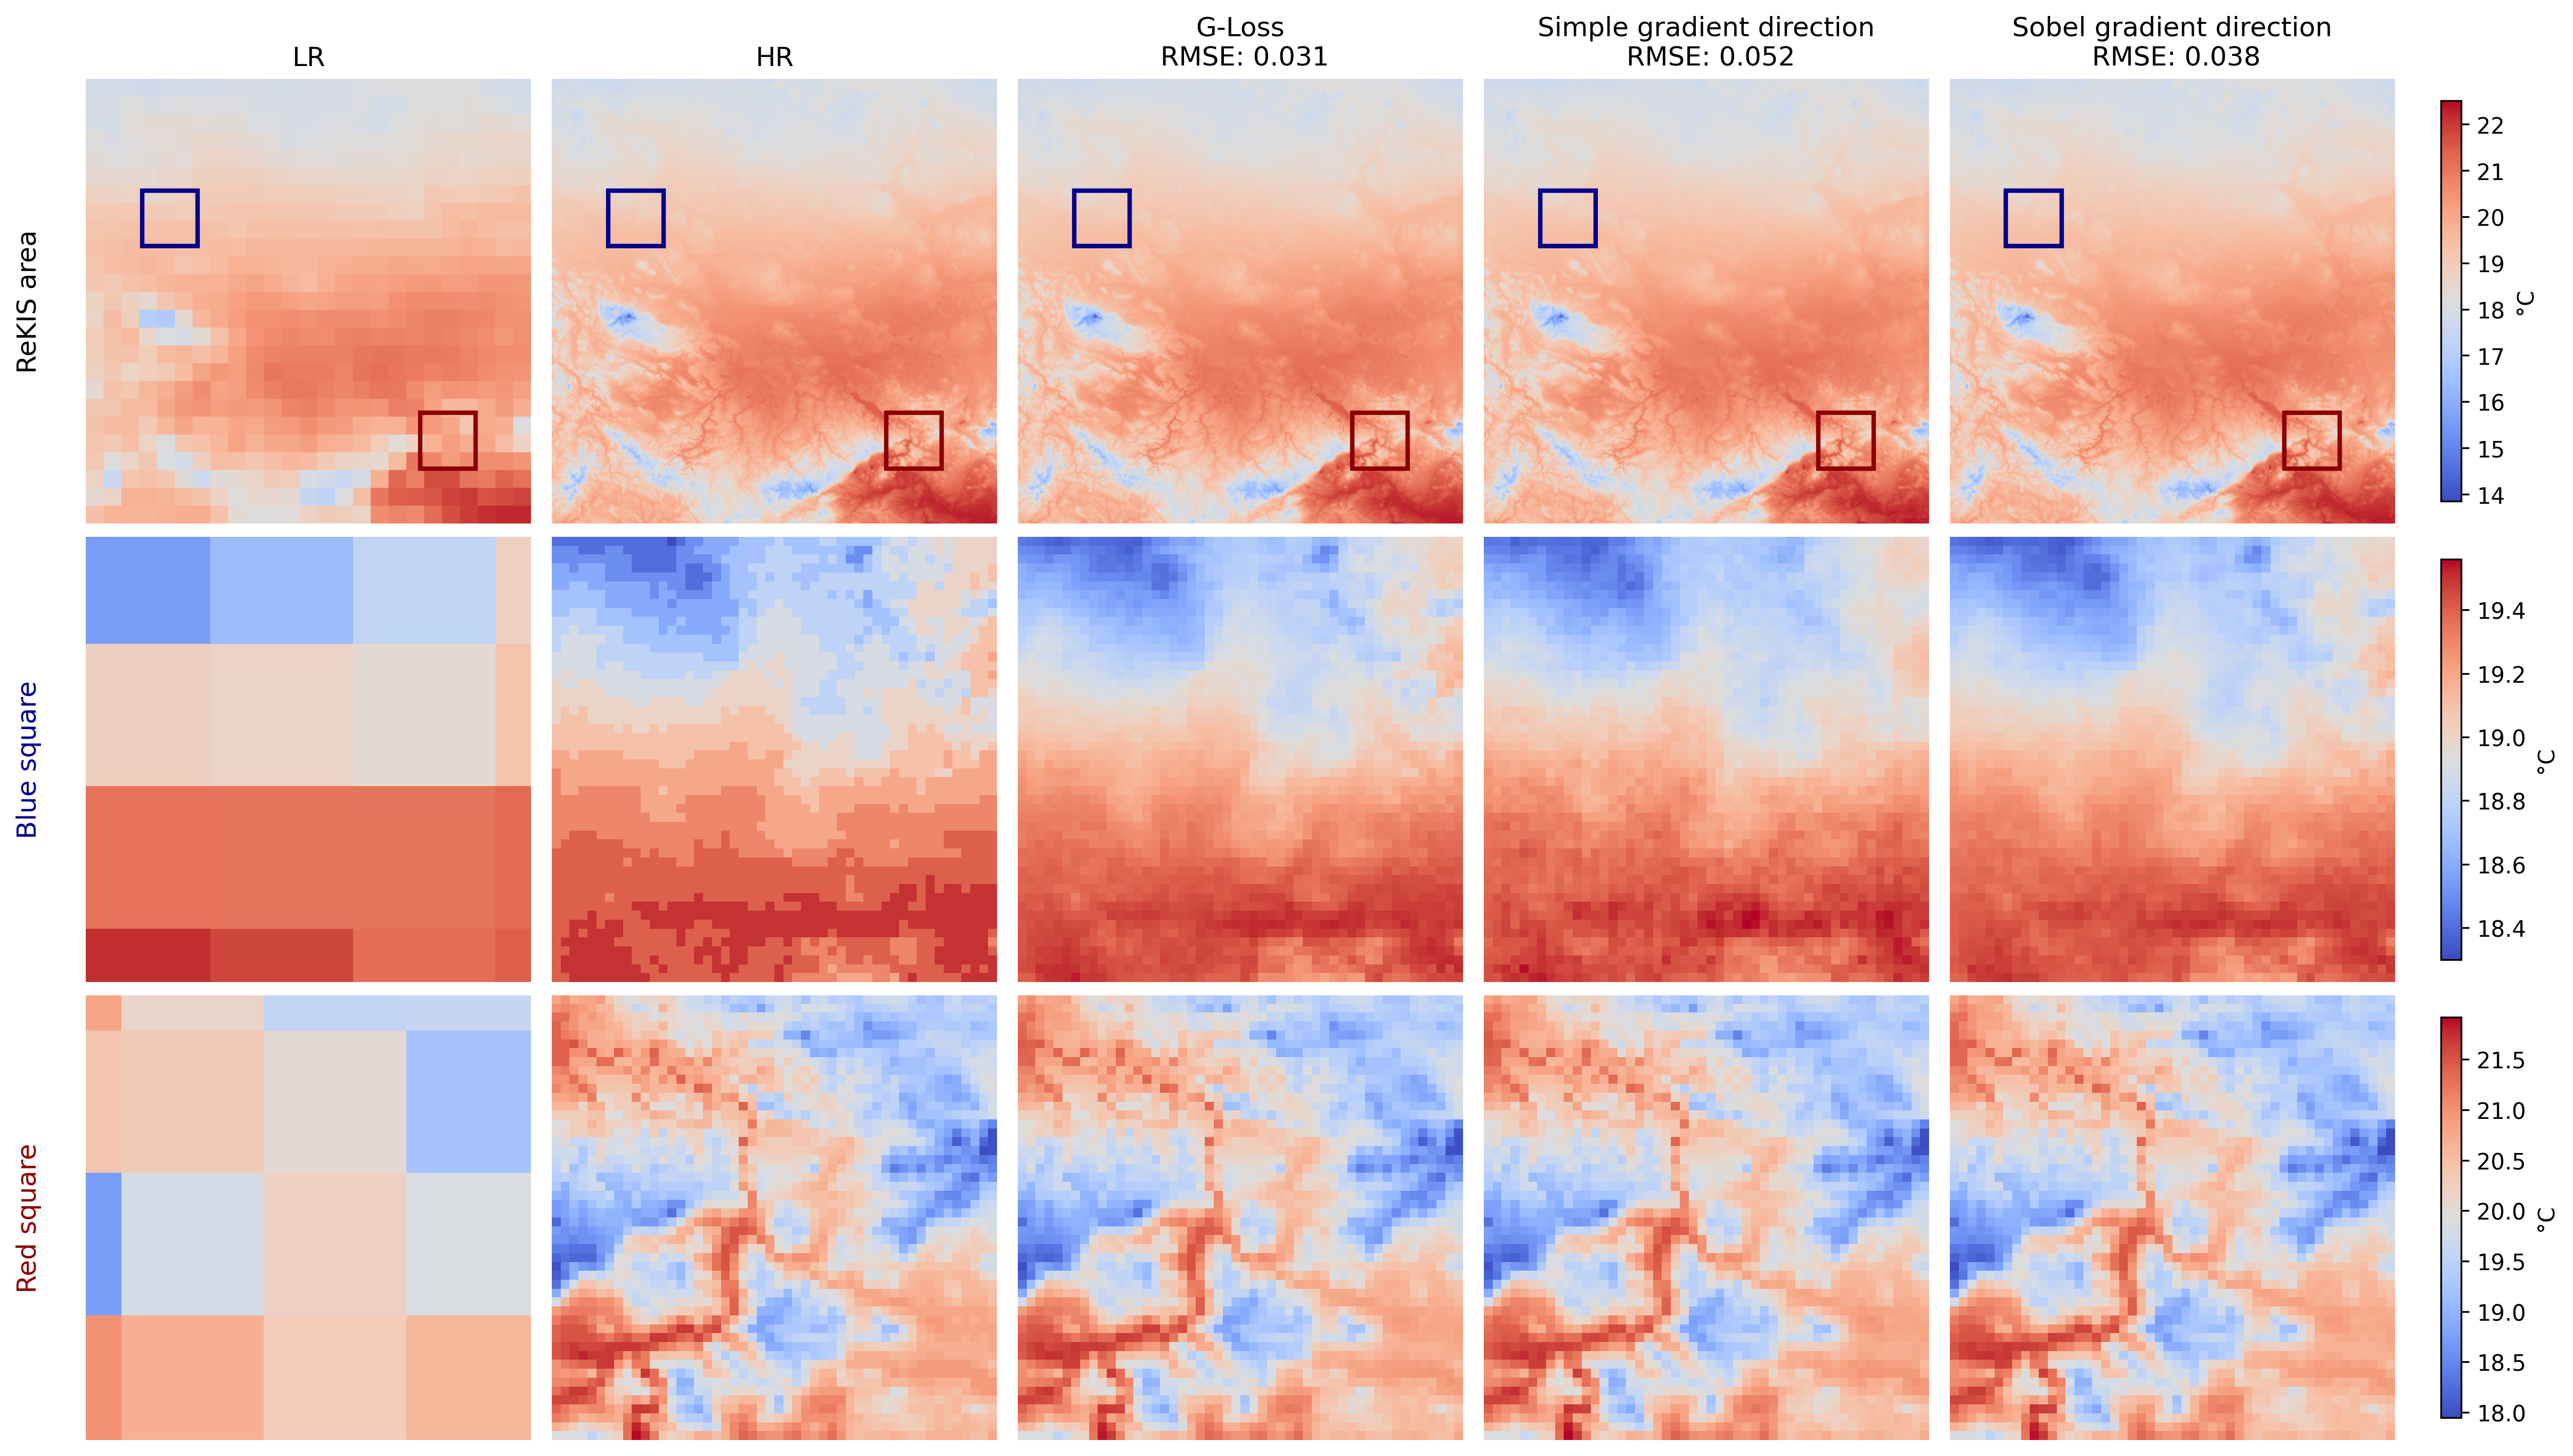
\includegraphics[width=0.88\linewidth]{images/soft_types_comp.png}
        \caption[Soft-constrained model types -- output visual comparison]{
        Soft-constrained model types -- output visual comparison. 
        The models are from Section~\ref{s:constraints_exp}. 
        The soft constraint on the gradient direction when using simple kernels results in a noisy output, as seen in the blue square. 
        In contrast, the Sobel variant generates a more compact result. This can be caused by the derivative kernels: Sobel kernels capture information over a larger neighborhood, making them more robust to noise. 
        G-Loss and Sobel gradient direction constraints are almost identical, however the G-Loss produces slightly more intense outputs in the top right corner of the blue square.
        Images correspond to the date 2005-08-18.}
        \label{fig:soft_types_comp}
    \end{figure}
\end{landscape}


\begin{landscape}
    \begin{figure}
    \centering
    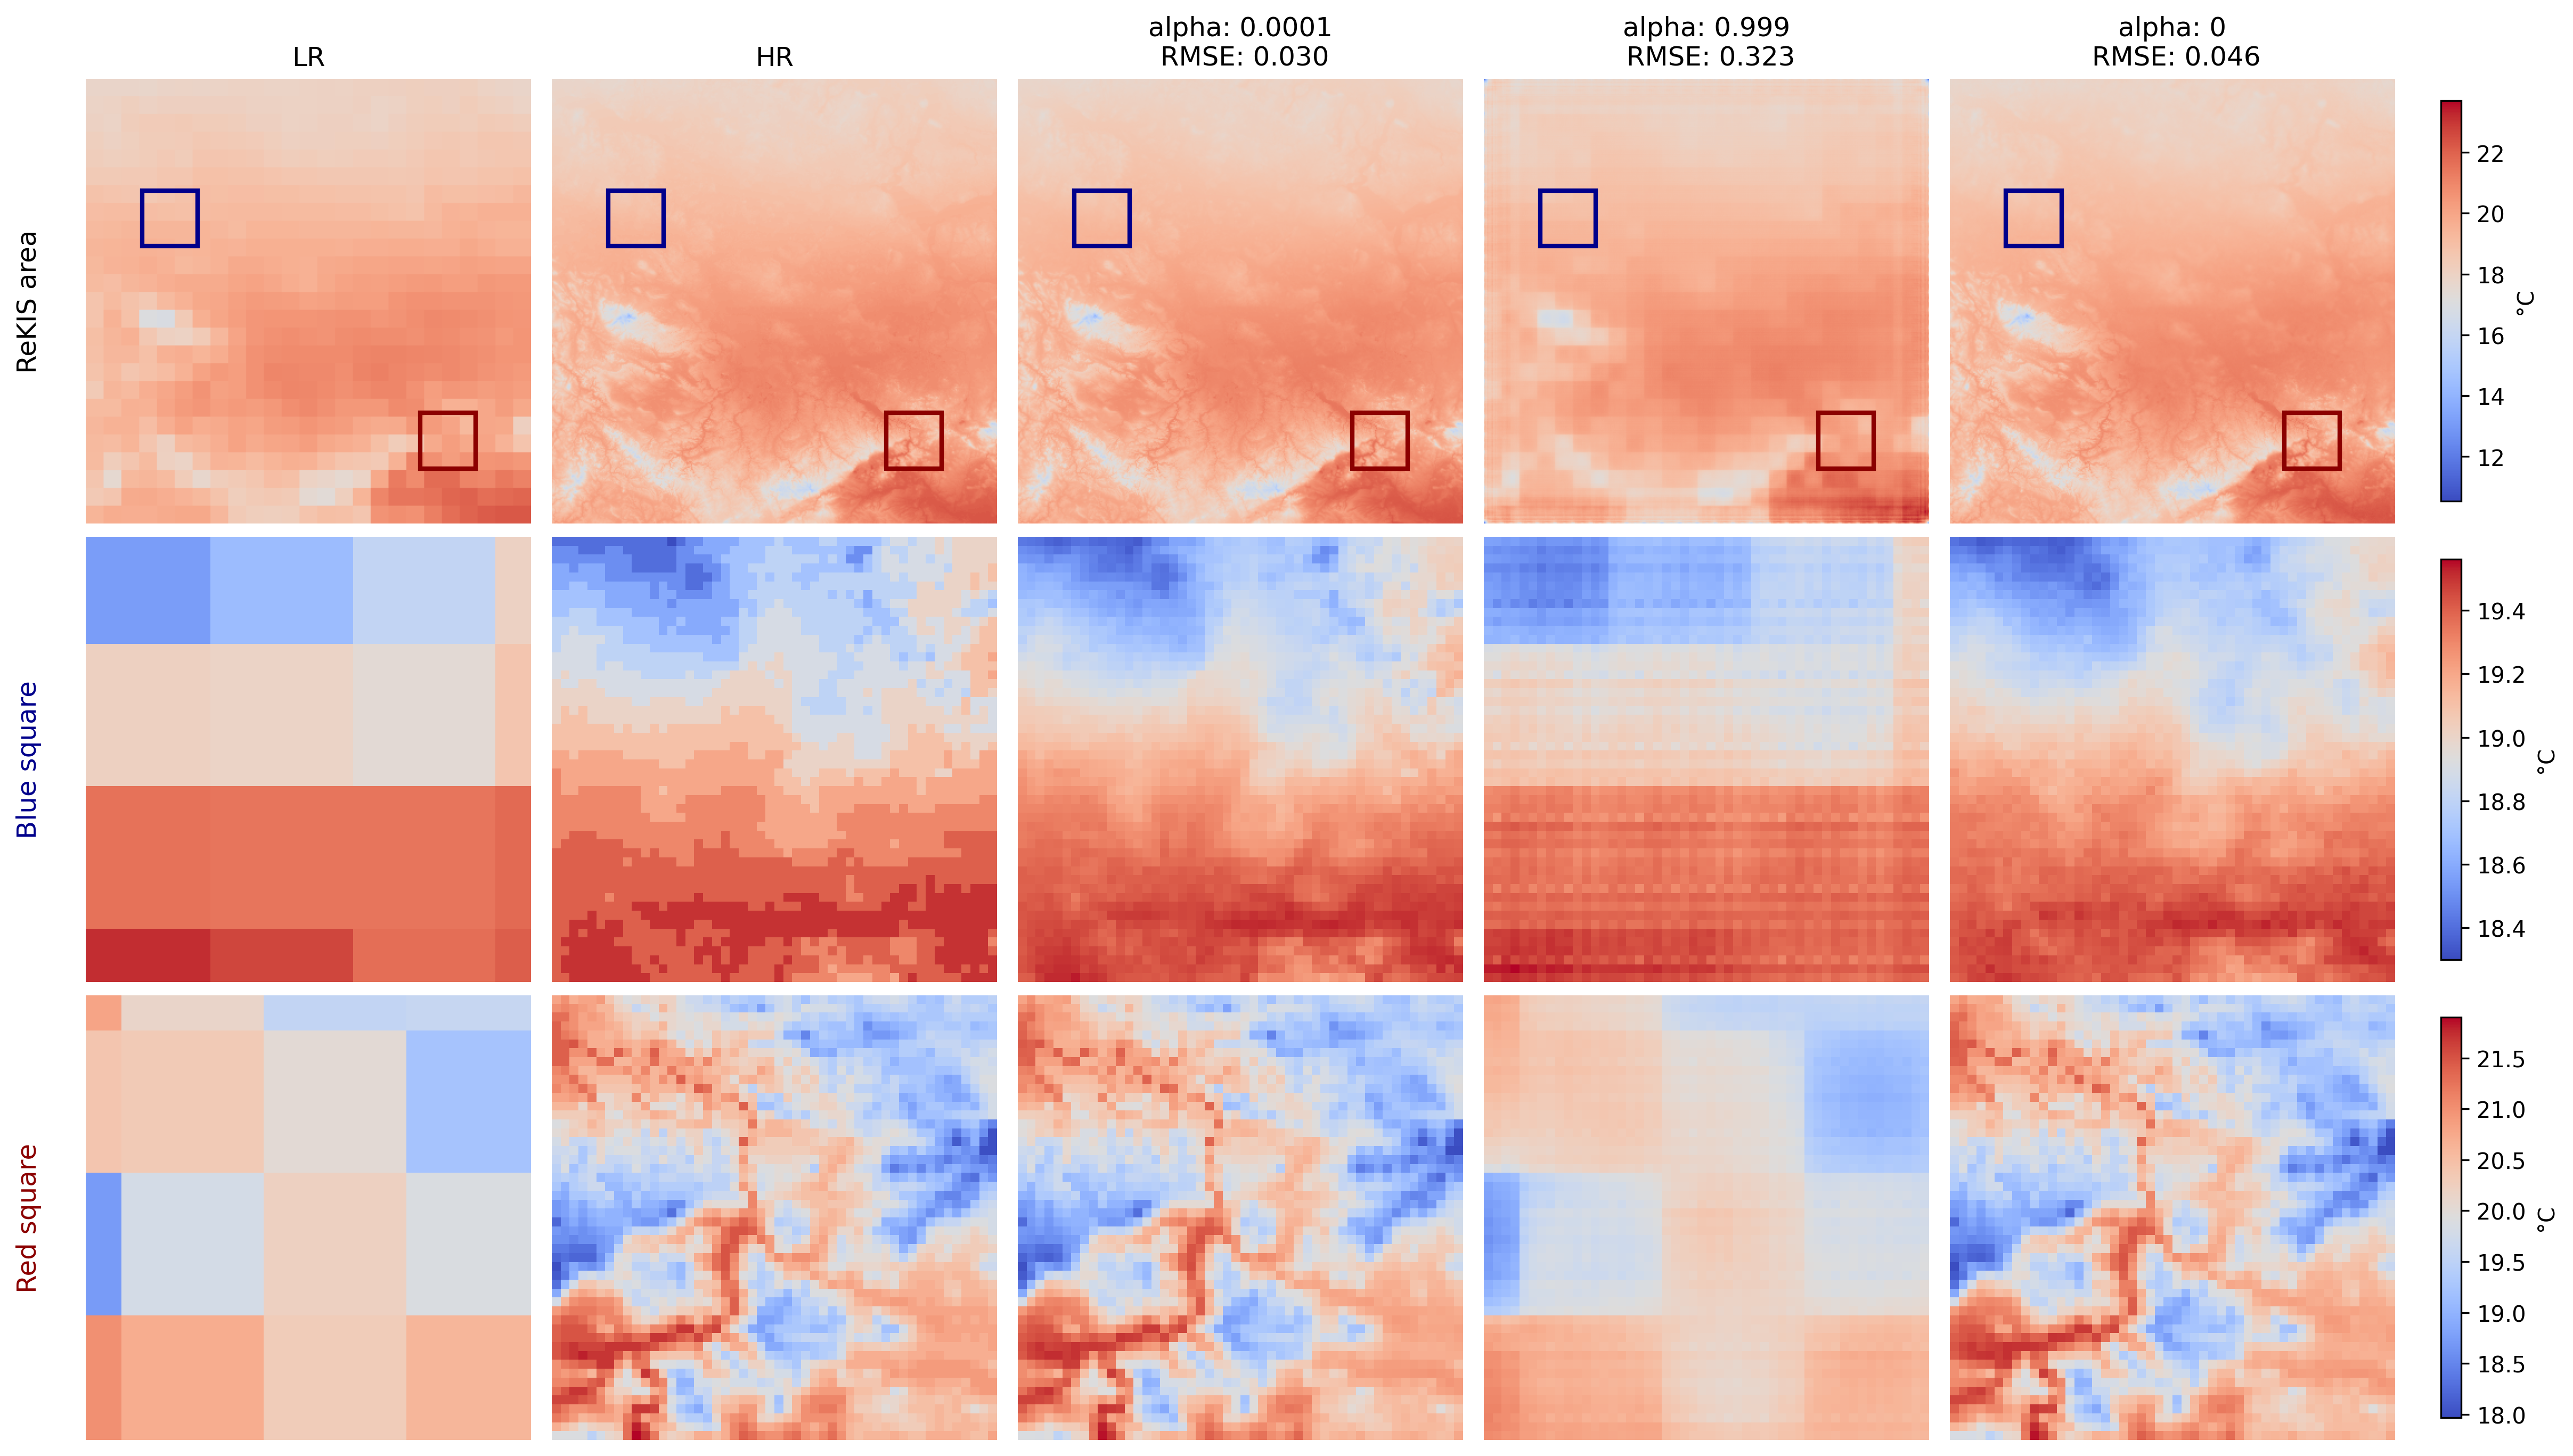
\includegraphics[width=0.88\linewidth]{images/alphas_comp.png}
    \caption[Alpha values experiment -- output visual comparison]{
    Alpha values experiment -- output visual comparison. The models are from Section~\ref{s:soft_constraints_alpha_exp}. 
    The model with alpha equal to 0.999 is producing noisier LR-like output. 
    A too large alpha value forces the model to strictly preserve the average between pixels, which results in merely reproducing the input, since the pixel-wise error contributes only weakly to the loss function. 
    The blue area of the model with alpha set to 0.0001 appears slightly more intense, than in the unconstrained model, particularly in the upper-right corner where three blue dots are located.
    Images correspond to the date 2005-08-18.}
    \label{fig:alphas_comp}
\end{figure}
\end{landscape}

\begin{landscape}
    \begin{figure}
    \centering
    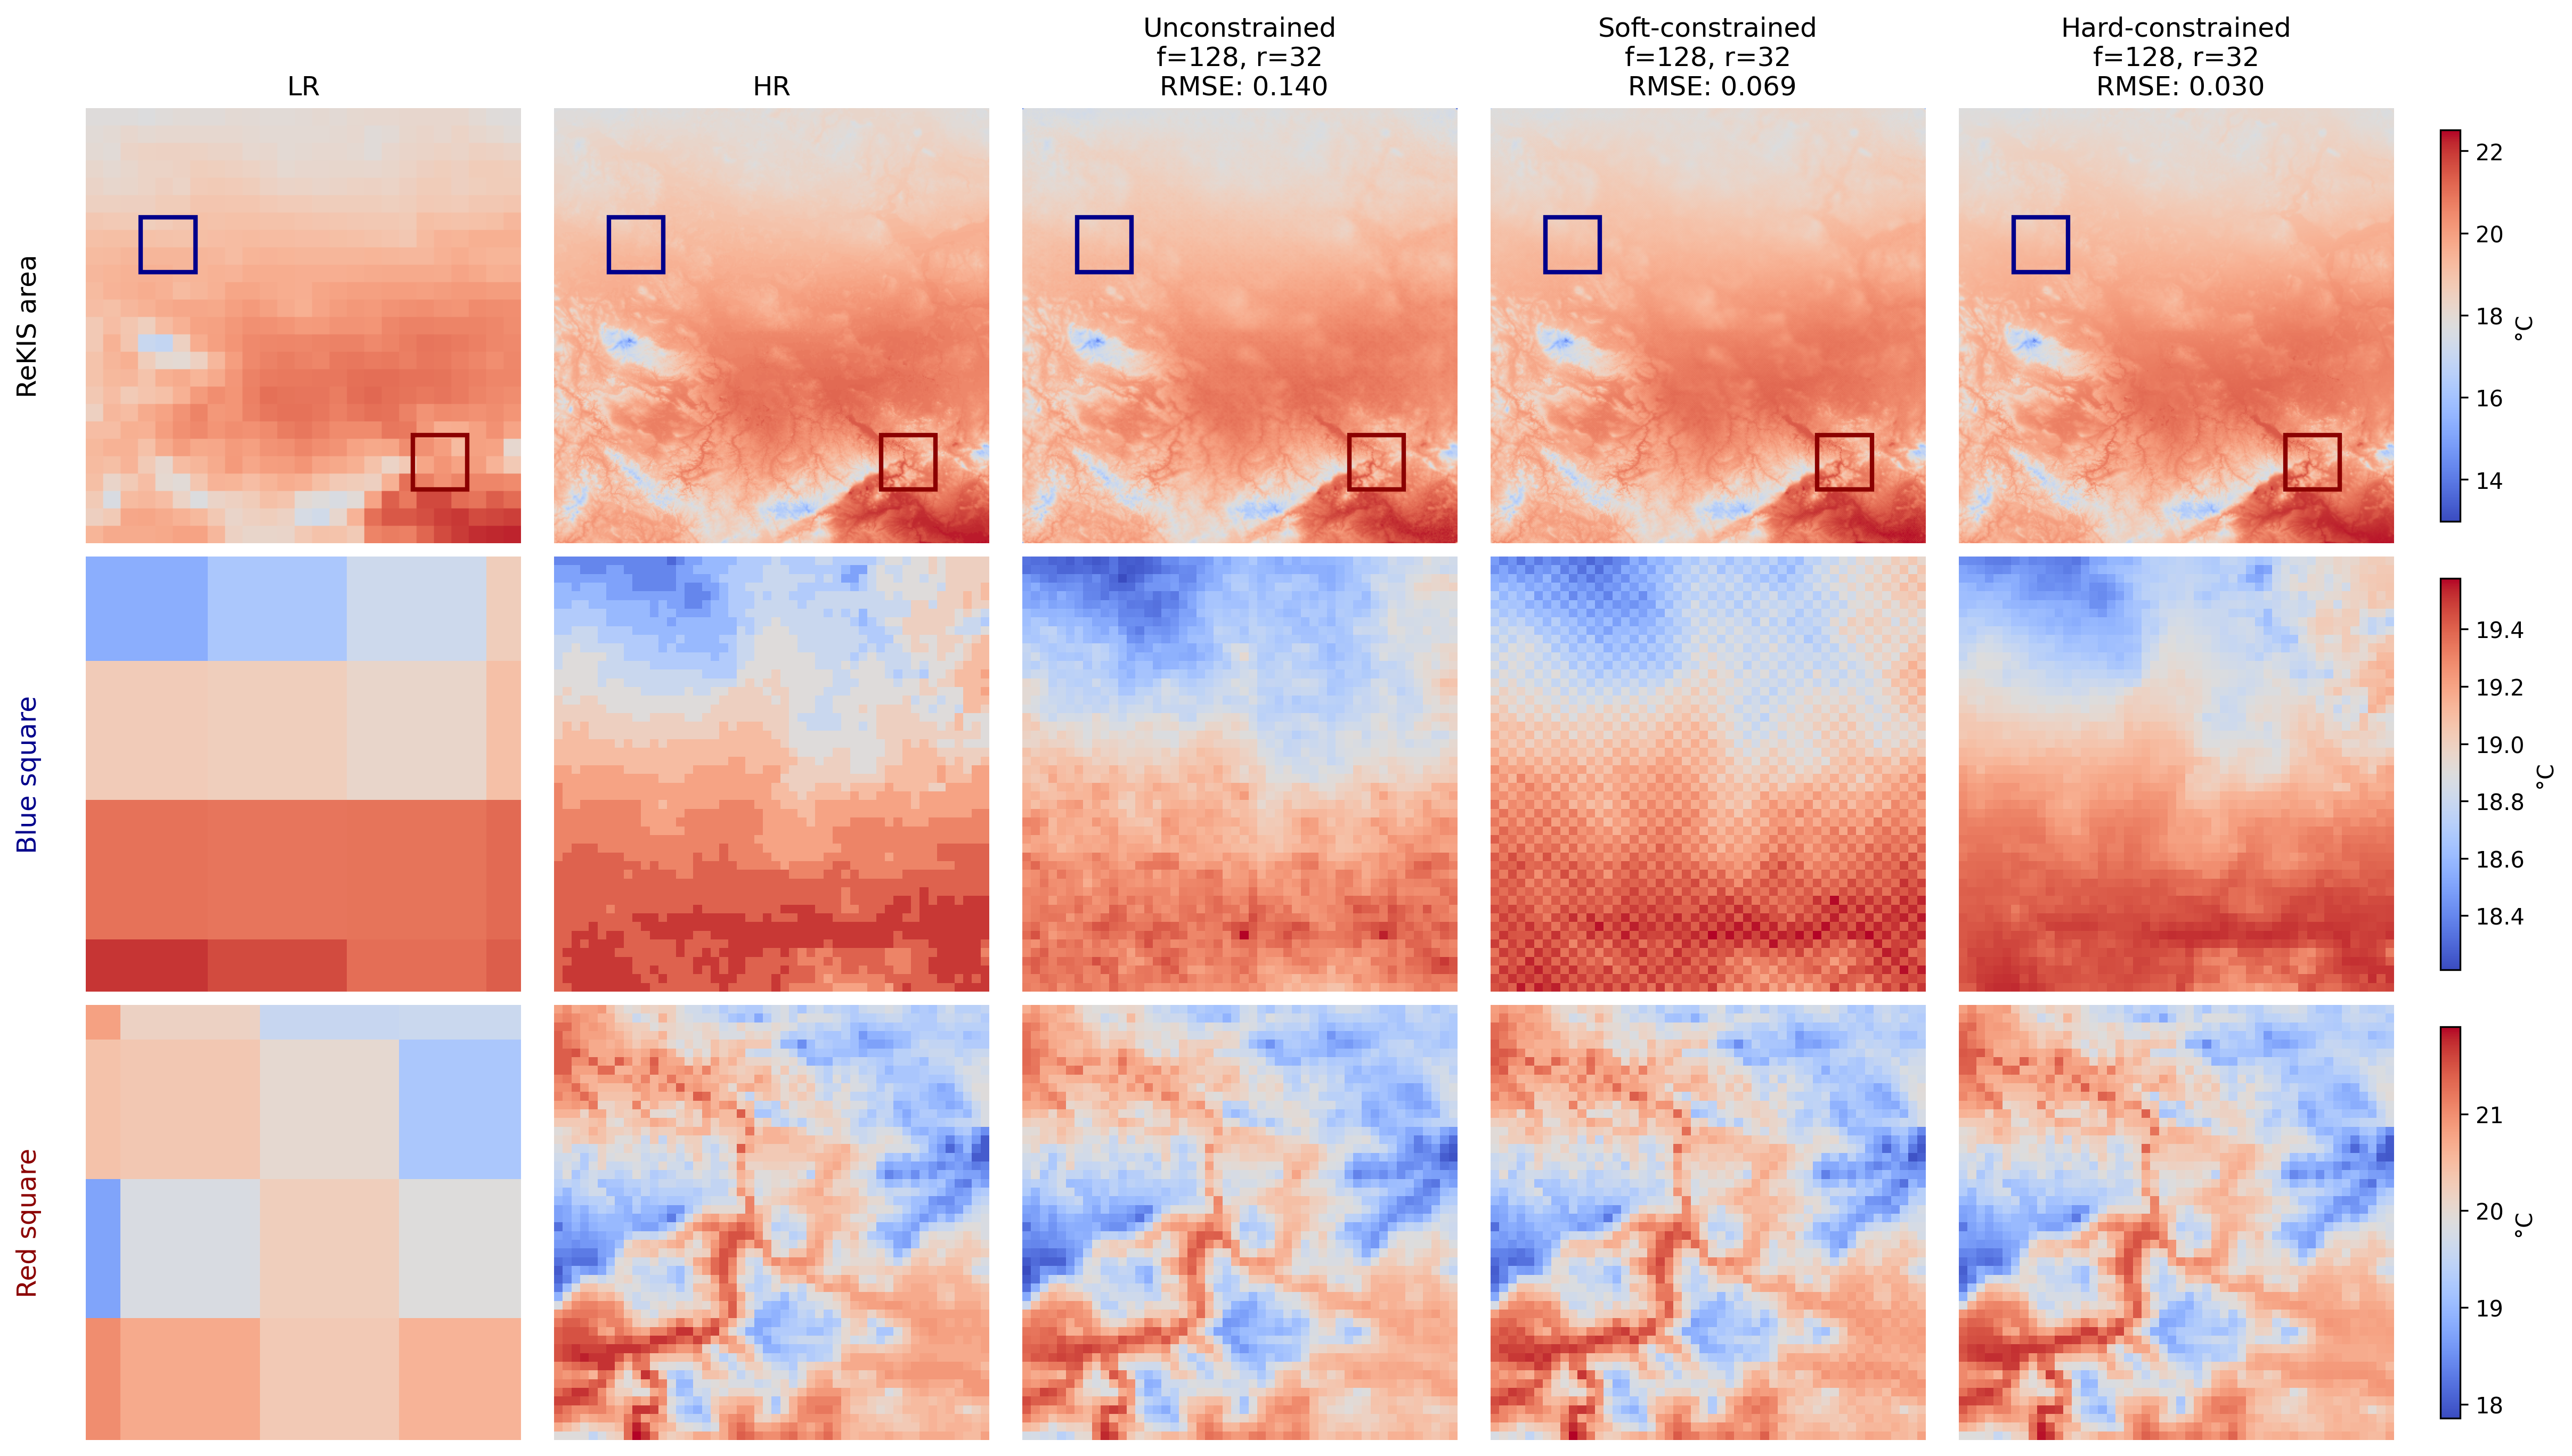
\includegraphics[width=0.88\linewidth]{images/constraint_type_comp.png}
    \caption[Constraint types -- output visual comparison]{
    Constraint types -- output visual comparison. The models are from Section~\ref{s:models_size_exp}. 
    Graining can be observed in the outputs of both the unconstrained and soft-constrained models. 
    In the unconstrained setting, the this looks like random noise, whereas under the soft-constraint it becomes more structured, almost grid-like. 
    This pattern can arise from comparing the means with the LR input. 
    The hard-constrained model produces the smoothest outcome, exhibiting minimal to no noise.
    Images correspond to the date 2005-08-18.}
    \label{fig:constraint_type_comp}
\end{figure}
\end{landscape}

\begin{landscape}
    \begin{figure}
    \centering
    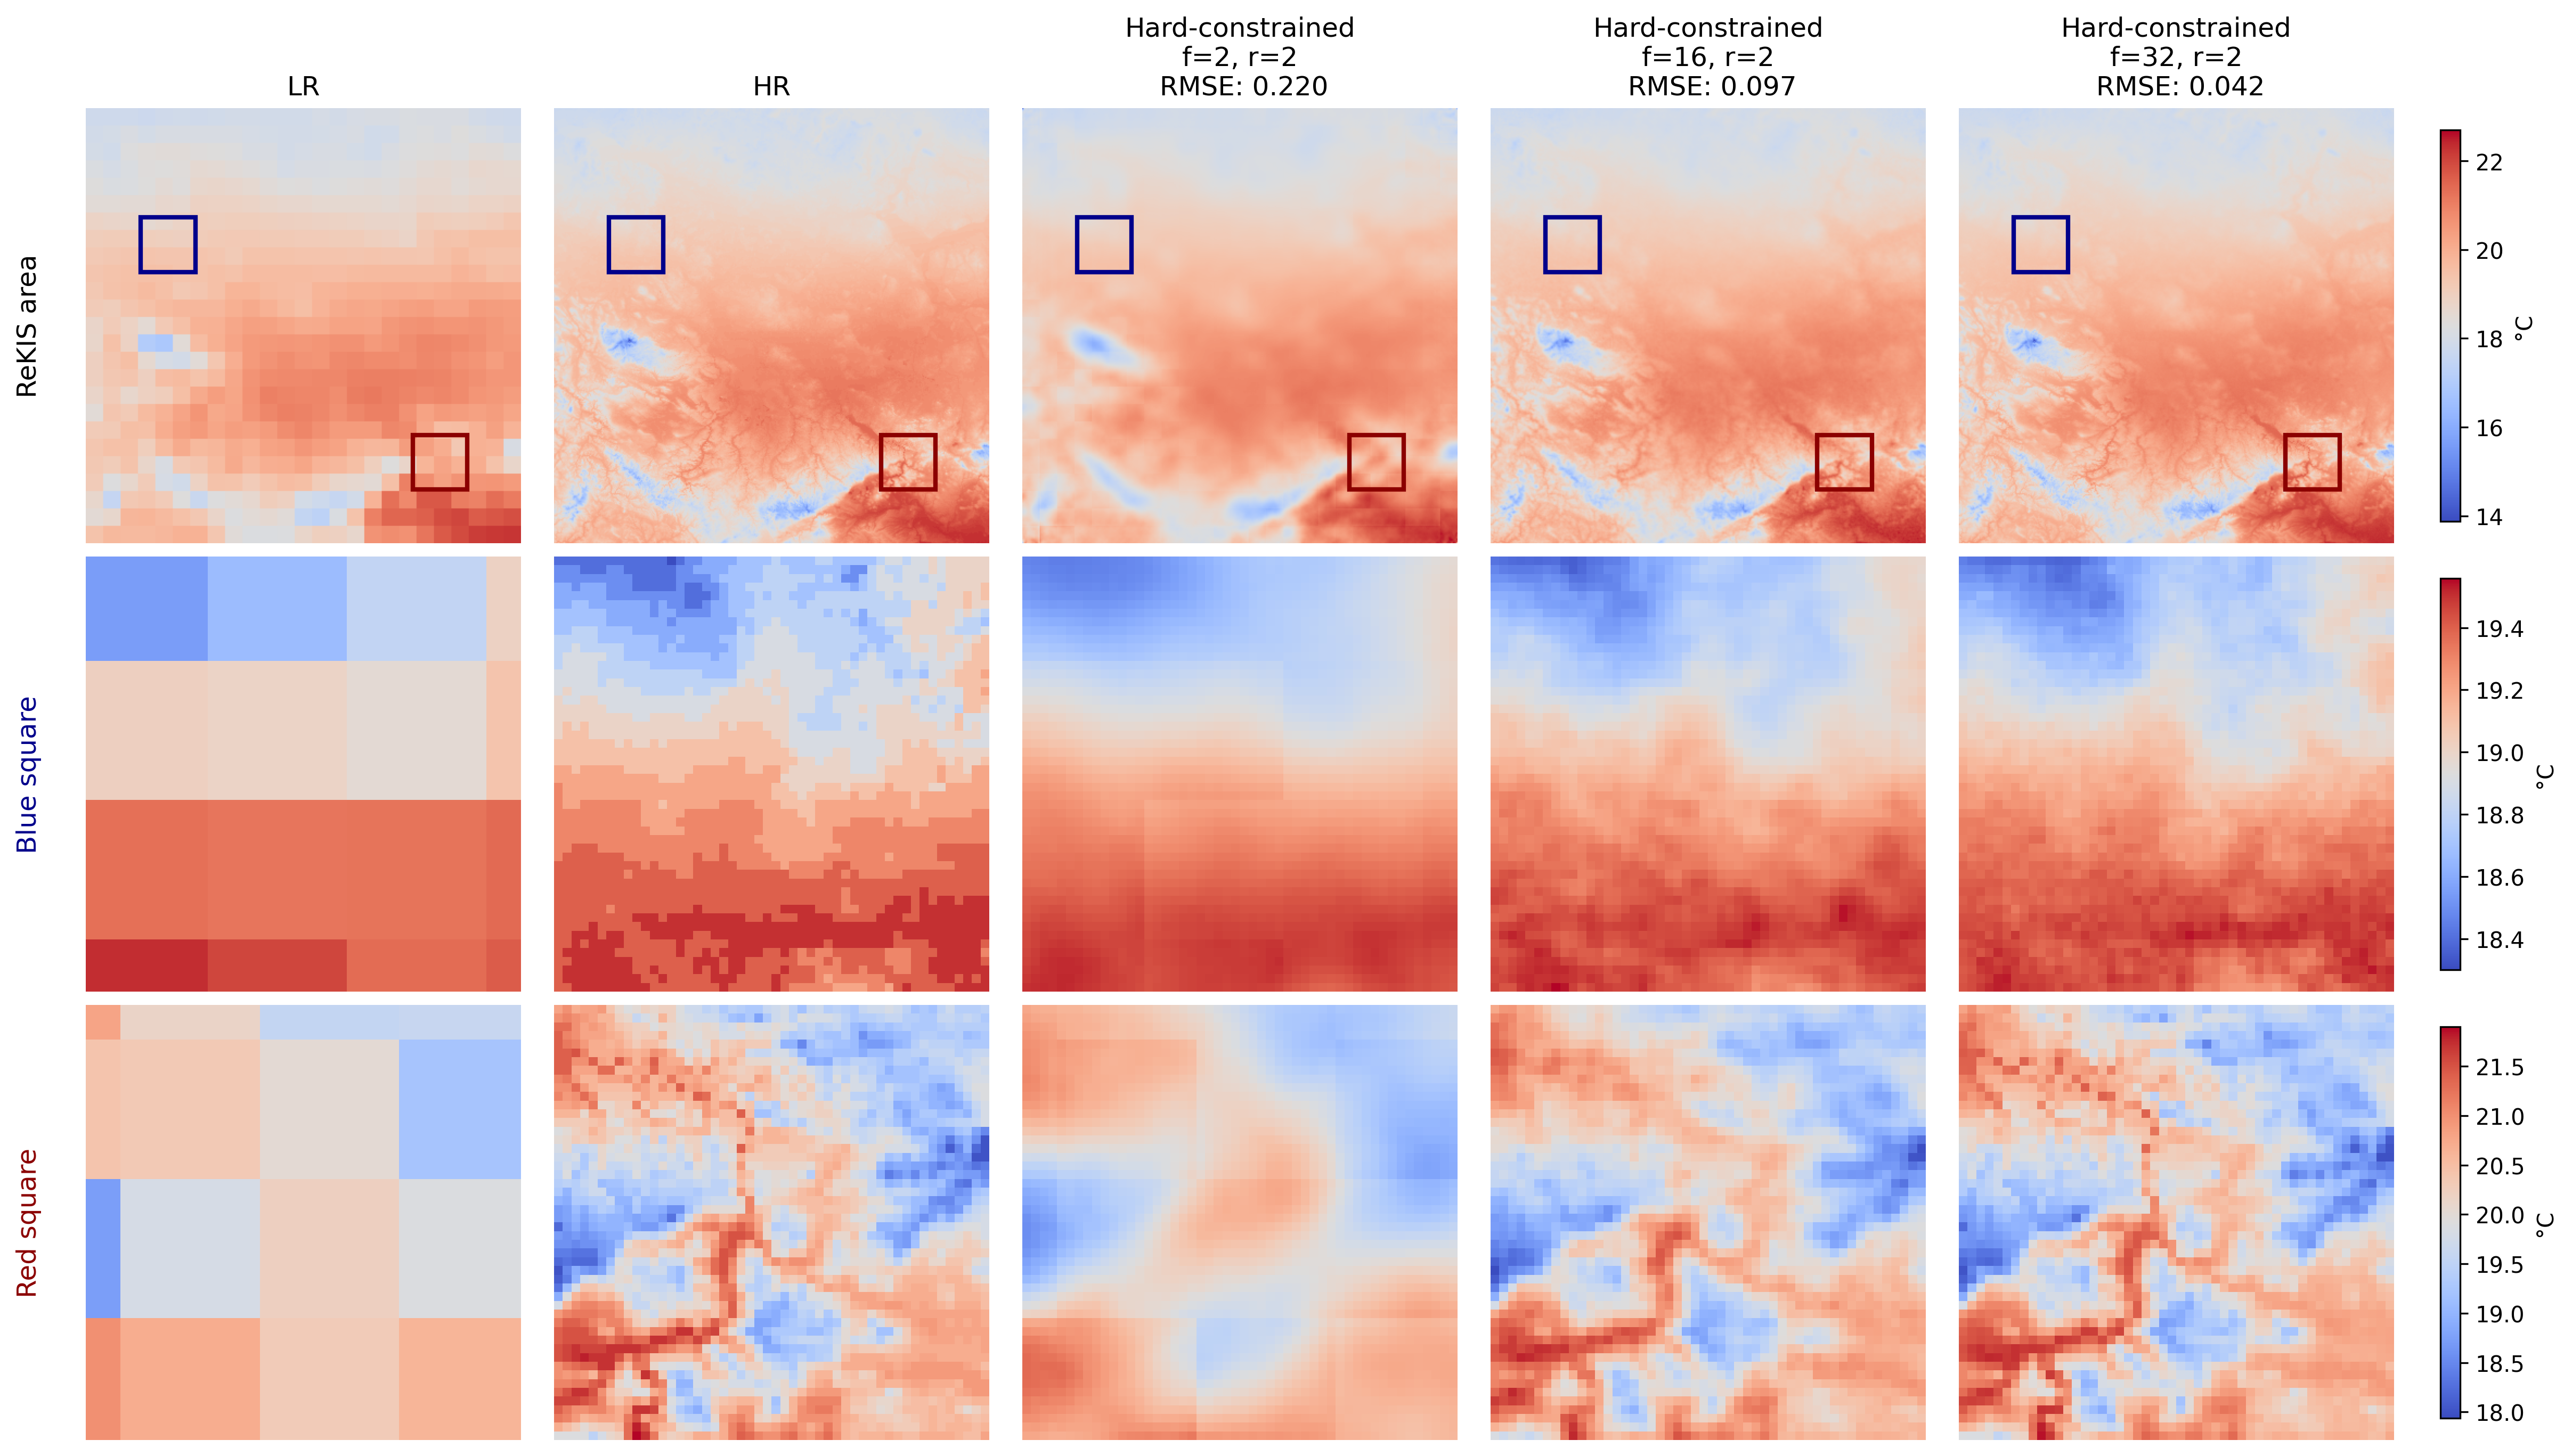
\includegraphics[width=0.88\linewidth]{images/sizes_comp.png}
    \caption[Hard-constrained different sized models -- output visual comparison]{
    Hard-constrained different sized models -- output visual comparison. 
    The models are from Section~\ref{s:models_size_exp}. 
    The smaller model to the left produces blurred images. 
    The more complex the models become, the more sharp their output appears to be.
    Images correspond to the date 2005-08-18.}
    \label{fig:sizes_comp}
\end{figure}
\end{landscape}
 % include `appendix.tex' from `text/' subdirectory

\backmatter % do not remove this command

\printbibliography % print out the BibLaTeX-generated bibliography list

\chapter{Contents of the attachment}

	\dirtree{%
		.1 /.
		.2 SISR-downscaling.
        .3 config\DTcomment{experiment configuration files}.
        .3 notebooks\DTcomment{supplementary Jupyter notebooks}.
        .3 scripts\DTcomment{additional scripts}.
		.3 src\DTcomment{source code}.
		.3 thesis\DTcomment{thesis in \LaTeX{}}.
        .3 README.md\DTcomment{description of the SISR-downscaling repository}.
		.2 text.
		.3 thesis.pdf\DTcomment{thesis in PDF}.
        .2 example\DTcomment{modifiable notebook to experiment with}.
	}
 % include `medium.tex' from `text/' subdirectory

\end{document}
